\documentclass[9pt,a4paper]{article}
\usepackage[margin=1.8cm,top=2.0cm,bottom=2.0cm]{geometry}
\usepackage{booktabs,colortbl,xcolor,array,makecell,hhline}
\usepackage{amsmath,amssymb}
\usepackage{helvet}\renewcommand{\familydefault}{\sfdefault}
\usepackage{fancyhdr,graphicx}
\usepackage[colorlinks=true,linkcolor=primary,urlcolor=primary,
            bookmarks=true,pdfborder={0 0 0}]{hyperref}
\usepackage{parskip,enumitem,titlesec,needspace}
\setlength{\parskip}{2pt}
\definecolor{passgreen}{RGB}{198,239,206}
\definecolor{failred}{RGB}{255,199,206}
\definecolor{warnamber}{RGB}{255,235,156}
\definecolor{r2green}{RGB}{198,239,206}
\definecolor{r2amber}{RGB}{255,235,156}
\definecolor{primary}{RGB}{0,70,127}
\definecolor{sepgray}{RGB}{130,130,130}
\titleformat{\section}{\normalsize\bfseries\color{primary}}{}{0em}{}
            [\vspace{-4pt}\textcolor{primary}{\rule{\linewidth}{0.5pt}}]
\titlespacing{\section}{0pt}{16pt}{6pt}
\newcommand{\exhead}[1]{%
  \medskip\noindent{\small\bfseries\color{primary}#1}%
  \par\vspace{-5pt}\noindent\textcolor{primary}{\rule{\linewidth}{0.4pt}}\vspace{2pt}}
\pagestyle{fancy}\fancyhf{}
\lhead{\small\textcolor{primary}{\textbf{Surrogate Factory}}}
\chead{\small\textcolor{sepgray}{CONFIDENTIAL}}
\rhead{\small\textcolor{primary}{UCAIRFOILS\_1}}
\lfoot{\small\textcolor{sepgray}{Surrogate Factory v2.2 --- Automated Validation Report}}
\rfoot{\small\thepage}
\renewcommand{\headrulewidth}{0.4pt}\renewcommand{\footrulewidth}{0.4pt}
\begin{document}
% ==== EXECUTIVE SUMMARY ====
\thispagestyle{fancy}

\begin{center}
  {\large\bfseries\color{primary} Executive Summary --- Surrogate Model Validation Report}\\[2pt]
  {\small\color{sepgray} Use case: \textbf{UCAIRFOILS\_1} \quad|\quad 07 September 2026 \quad|\quad 1 model(s)}
\end{center}
\vspace{-4pt}\noindent\rule{\linewidth}{1pt}\vspace{3pt}

\begin{center}
\colorbox{warnamber}{\begin{minipage}{0.66\linewidth}
  \vspace{5pt}\centering
  {\normalsize\bfseries REQUIREMENTS PARTIALLY MET}\\[4pt]
  {\small\bfseries Recommended model:} {\small MLP}\\[5pt]
\colorbox{r2green}{\begin{minipage}{0.97\linewidth}\vspace{2pt}\centering {\small\bfseries Avg R\textsuperscript{2}: 0.9908} \enspace---\enspace {\small Excellent}\vspace{2pt}\end{minipage}}\\[2pt]
\colorbox{warnamber}{\begin{minipage}{0.97\linewidth}\vspace{2pt}\centering {\small\bfseries Q90 Accuracy} \enspace---\enspace {\small Partially met}\\[1pt]{\footnotesize Pass: CD}\\[1pt]{\footnotesize\color{red} Fail: CL, CM, top\_transition\_location, bottom\_transition\_location}\vspace{2pt}\end{minipage}}
  \vspace{5pt}
\end{minipage}}
\end{center}

\section{Project Overview}
\renewcommand{\arraystretch}{1.2}
\begin{tabular}{|l|p{0.60\linewidth}|}
  \hline
  \textbf{Use case}           & UCAIRFOILS\_1 \\ \hline
  \textbf{Inputs}             & alpha, log10\_Re, uW1, uW2, uW3, uW4, uW5, uW6, uW7, uW8, lW1, lW2, lW3, lW4, lW5, lW6, lW7, lW8, TE\_thickness, LE\_weight \\ \hline
  \textbf{Outputs}            & 5: CL, CD, CM, top\_transition\_location, bottom\_transition\_location \\ \hline
  \textbf{Train / Val / Test} & 80\% / 10\% / 10\% \\ \hline
  \textbf{Accuracy target}    & Q90 $<$ 10\% relative error per output \\ \hline
\end{tabular}

\par\begin{minipage}{\linewidth}
\section{Variable Correlation --- Input vs Output}
\begin{center}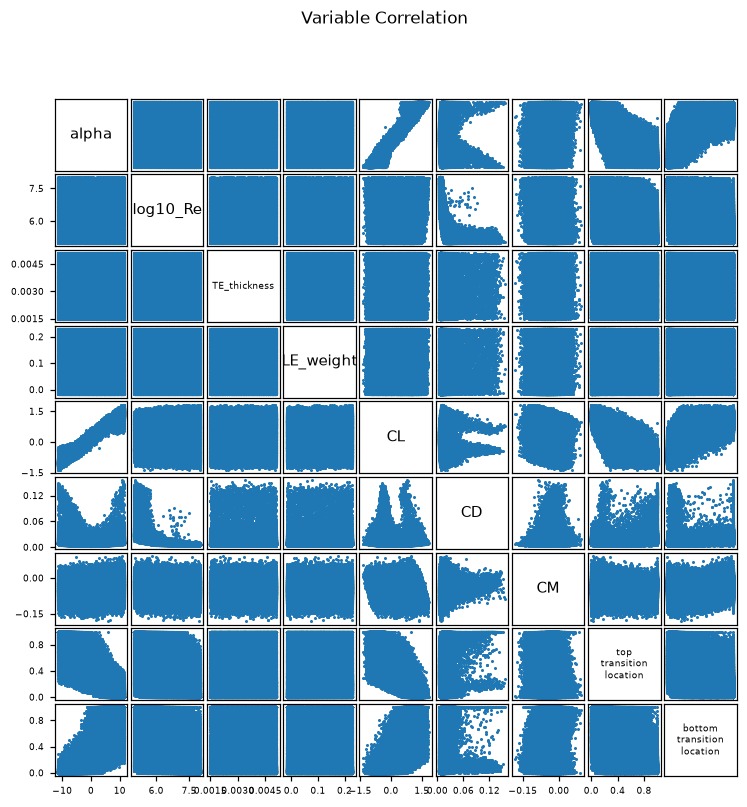
\includegraphics[width=0.80\linewidth,height=0.46\textheight,keepaspectratio]{analysis_plots/data_scatter_vars.png}\end{center}
\end{minipage}\par\medskip
\section{Data Statistics}
Per-variable statistics over all data (train + val + test), as \texttt{Train\_set.describe()} reports them in the feature-selection notebook: count, mean, standard deviation, minimum, quartiles and maximum.

\par\begin{minipage}{\linewidth}
\exhead{Inputs}
\begin{center}
\footnotesize
\renewcommand{\arraystretch}{1.15}
\resizebox{\linewidth}{!}{%
\begin{tabular}{|l|r|r|r|r|r|r|r|r|}
\hline
\textbf{} & \textbf{count} & \textbf{mean} & \textbf{std} & \textbf{min} & \textbf{P25} & \textbf{P50} & \textbf{P75} & \textbf{max} \\ \hline
\textbf{alpha} & 119,756 & 0.7531 & 6.3925 & -11.4586 & -4.5034 & 1.1937 & 6.1528 & 11.4591 \\ \hline
\textbf{log10\_Re} & 119,756 & 6.5225 & 0.8611 & 5 & 5.7864 & 6.5347 & 7.2648 & 8 \\ \hline
\textbf{uW1} & 119,756 & 0.2303 & 0.0748 & 0.1 & 0.1657 & 0.2304 & 0.295 & 0.36 \\ \hline
\textbf{uW2} & 119,756 & 0.2299 & 0.075 & 0.1 & 0.1651 & 0.2299 & 0.2947 & 0.36 \\ \hline
\textbf{uW3} & 119,756 & 0.23 & 0.075 & 0.1 & 0.1651 & 0.2301 & 0.295 & 0.36 \\ \hline
\textbf{uW4} & 119,756 & 0.23 & 0.075 & 0.1 & 0.1651 & 0.23 & 0.295 & 0.36 \\ \hline
\textbf{uW5} & 119,756 & 0.23 & 0.075 & 0.1 & 0.165 & 0.2299 & 0.2949 & 0.36 \\ \hline
\textbf{uW6} & 119,756 & 0.23 & 0.075 & 0.1 & 0.1652 & 0.2299 & 0.295 & 0.36 \\ \hline
\textbf{uW7} & 119,756 & 0.2299 & 0.075 & 0.1 & 0.165 & 0.2299 & 0.2949 & 0.36 \\ \hline
\textbf{uW8} & 119,756 & 0.2301 & 0.075 & 0.1 & 0.1652 & 0.2302 & 0.2951 & 0.36 \\ \hline
\textbf{lW1} & 119,756 & -0.1923 & 0.0877 & -0.34 & -0.2674 & -0.1947 & -0.1207 & 0.0872 \\ \hline
\textbf{lW2} & 119,756 & -0.1105 & 0.1346 & -0.34 & -0.2269 & -0.1128 & 0.0044 & 0.13 \\ \hline
\textbf{lW3} & 119,756 & -0.1052 & 0.1354 & -0.34 & -0.2223 & -0.1051 & 0.0118 & 0.13 \\ \hline
\textbf{lW4} & 119,756 & -0.1045 & 0.1356 & -0.34 & -0.2218 & -0.1042 & 0.013 & 0.13 \\ \hline
\textbf{lW5} & 119,756 & -0.1048 & 0.1356 & -0.34 & -0.2222 & -0.1046 & 0.0125 & 0.13 \\ \hline
\textbf{lW6} & 119,756 & -0.1051 & 0.1356 & -0.34 & -0.2223 & -0.1051 & 0.0123 & 0.13 \\ \hline
\textbf{lW7} & 119,756 & -0.1046 & 0.1356 & -0.34 & -0.2219 & -0.1043 & 0.0128 & 0.13 \\ \hline
\textbf{lW8} & 119,756 & -0.1044 & 0.1355 & -0.34 & -0.2215 & -0.104 & 0.0129 & 0.13 \\ \hline
\textbf{TE\_thickness} & 119,756 & 0.0033 & 0.001 & 0.0015 & 0.0024 & 0.0033 & 0.0042 & 0.0051 \\ \hline
\textbf{LE\_weight} & 119,756 & 0.1045 & 0.0715 & -0.018 & 0.0425 & 0.1038 & 0.1663 & 0.23 \\ \hline
\end{tabular}
}
\par\vspace{2pt}
{\scriptsize Input variables — Train\_set.describe()}
\end{center}
\end{minipage}\par\medskip
\par\begin{minipage}{\linewidth}
\exhead{Outputs}
\begin{center}
\footnotesize
\renewcommand{\arraystretch}{1.15}
\resizebox{\linewidth}{!}{%
\begin{tabular}{|l|r|r|r|r|r|r|r|r|}
\hline
\textbf{} & \textbf{count} & \textbf{mean} & \textbf{std} & \textbf{min} & \textbf{P25} & \textbf{P50} & \textbf{P75} & \textbf{max} \\ \hline
\textbf{CL} & 119,756 & 0.3298 & 0.7075 & -1.3751 & -0.2552 & 0.3931 & 0.9308 & 1.8332 \\ \hline
\textbf{CD} & 119,756 & 0.013 & 0.0134 & 0.0035 & 0.0068 & 0.0091 & 0.0141 & 0.1555 \\ \hline
\textbf{CM} & 119,756 & -0.0444 & 0.0341 & -0.182 & -0.0676 & -0.044 & -0.0209 & 0.0925 \\ \hline
\textbf{top\_transition\_location} & 119,756 & 0.3748 & 0.2965 & 0 & 0.1243 & 0.2911 & 0.6017 & 1 \\ \hline
\textbf{bottom\_transition\_location} & 119,756 & 0.3432 & 0.3408 & 0 & 0.0483 & 0.2009 & 0.6041 & 1 \\ \hline
\end{tabular}
}
\par\vspace{2pt}
{\scriptsize Output variables — Train\_set.describe()}
\end{center}
\end{minipage}\par\medskip
\section{Model Selection}
\begin{minipage}{\linewidth}
\renewcommand{\arraystretch}{1.2}
\begin{tabular}{|l|r|r|r|}
  \hline
  \textbf{Model} & \textbf{Avg R\textsuperscript{2}} & \textbf{Q90 pass (5)} & \textbf{KS pass (5)} \\ \hline
  {\bfseries MLP\ $\star$} & {\bfseries 0.9908} & {\bfseries 1/5} & {\bfseries 0/5} \\ \hline
\end{tabular}
\par\vspace{4pt}
{\footnotesize $\star$ Recommended model.\enspace Q90 target: $<10\%$.\enspace KS: $p\geq 0.05$ = no overfitting.}
\end{minipage}

\section{Accuracy Assessment (Q90 \& R\textsuperscript{2})}
\begin{minipage}{\linewidth}
\renewcommand{\arraystretch}{1.2}
\begin{tabular}{l|rrr|}
  \hline
  \textbf{Output} & \multicolumn{3}{c|}{\textbf{MLP}\ $\star$} \\ \hline
  & R\textsuperscript{2} & Q90 & Gap \\ \hline
  CL & \cellcolor{r2green}0.9988 & \cellcolor{failred}0.1103 & \cellcolor{failred}+0.0103 \\ \hline
  CD & \cellcolor{r2green}0.9740 & \cellcolor{passgreen}0.0380 & \cellcolor{passgreen}-0.0620 \\ \hline
  CM & \cellcolor{r2green}0.9919 & \cellcolor{failred}0.2912 & \cellcolor{failred}+0.1912 \\ \hline
  top\_transition\_location & \cellcolor{r2green}0.9963 & \cellcolor{failred}0.1520 & \cellcolor{failred}+0.0520 \\ \hline
  bottom\_transition\_location & \cellcolor{r2green}0.9931 & \cellcolor{failred}0.2881 & \cellcolor{failred}+0.1881 \\ \hline
\end{tabular}
\par\vspace{4pt}
{\footnotesize \colorbox{r2green}{\ } R\textsuperscript{2}$\!\geq\!0.95$\enspace \colorbox{r2amber}{\ } R\textsuperscript{2}$\!\in[0.80,0.95)$\enspace \colorbox{failred}{\ } R\textsuperscript{2}$\!<\!0.80$ or Q90 fail\enspace \colorbox{passgreen}{\ } pass\enspace Gap$=$Q90$-$target ($<\!0\Rightarrow$ margin)}
\end{minipage}

\par\begin{minipage}{\linewidth}
\section{Training History}
\begin{center}
\includegraphics[width=0.70\linewidth,height=0.28\textheight,keepaspectratio]{../training_curve.png}\end{center}
{\footnotesize Training and validation loss per iteration, log scale. The validation curve is measured, not approximated: per epoch on the early-stopping split for the MLP, per stage on the validation split for gradient boosting (whose training curve is its per-stage deviance). Models saved before this was recorded fall back to the $(1-R^2)\cdot\mathrm{Var}(y)/2$ approximation.}\end{minipage}\par\medskip

\par\begin{minipage}{\linewidth}
\section{Predicted vs True --- MLP}
\begin{center}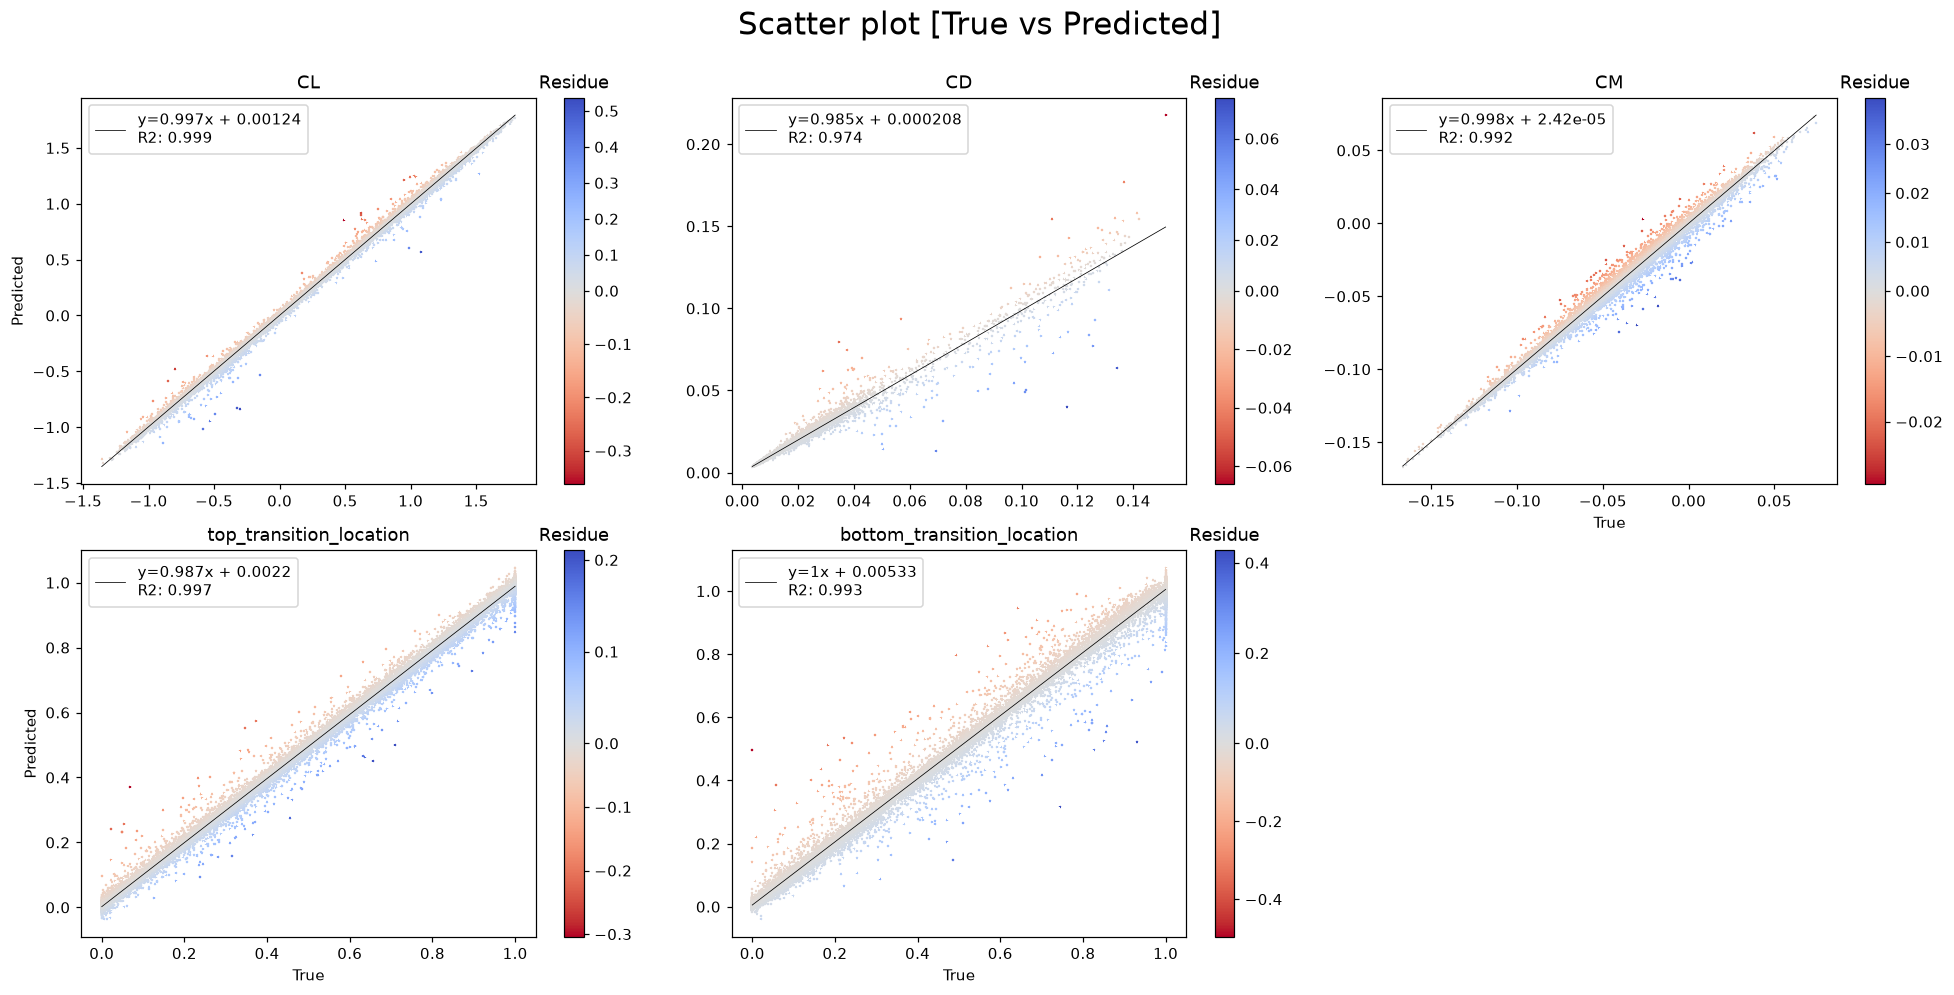
\includegraphics[width=\linewidth,height=0.80\textheight,keepaspectratio]{analysis_plots/winner_pred_true.png}\end{center}
\end{minipage}\par\medskip


\section{Data Split Quality}
\begin{minipage}{\linewidth}
\renewcommand{\arraystretch}{1.2}
\begin{tabular}{|l|r|c|}
  \hline\textbf{Metric} & \textbf{Value} & \textbf{Pass} \\ \hline
  Residual voxel proportion ($\leq\!0.05$) & 0.000 & \cellcolor{passgreen}$\checkmark$ \\ \hline
  Valid test proportion & 0.965 & \\ \hline
  p-hacking test proportion ($\leq\!0.05$ warn) & 0.003 & \cellcolor{passgreen}$\checkmark$ \\ \hline
  Isolated test proportion ($\leq\!0.05$ warn) & 0.033 & \cellcolor{passgreen}$\checkmark$ \\ \hline
  Chi\textsuperscript{2} p-value ($\geq\!0.05$) & \textemdash & \textemdash \\ \hline
\end{tabular}
\end{minipage}
\textcolor{passgreen!60!black}{\textbf{No p-hacking concern:}} only 0.2\% of test points lie closer to a training point than training points are to each other, so the test error is not flattered.

\section{Overfitting Check (KS Test) --- MLP}
\begin{minipage}{\linewidth}
\renewcommand{\arraystretch}{1.15}
\begin{tabular}{|l|r|}
  \hline\textbf{Output} & \textbf{KS p-value} \\ \hline
  CL & \cellcolor{failred}0.000 \\ \hline
  CD & \cellcolor{failred}0.000 \\ \hline
  CM & \cellcolor{failred}0.000 \\ \hline
  top\_transition\_location & \cellcolor{failred}0.000 \\ \hline
  bottom\_transition\_location & \cellcolor{failred}0.002 \\ \hline
\end{tabular}
\par\vspace{4pt}
{\footnotesize \colorbox{passgreen}{\ } $p\geq 0.05$ --- no overfitting\enspace \colorbox{failred}{\ } $p<0.05$ --- overfitting detected}
\end{minipage}
\clearpage
\thispagestyle{empty}
\vspace*{\fill}
\begin{center}
  \textcolor{sepgray}{\rule{0.40\linewidth}{1pt}}\\[20pt]
  {\Huge\bfseries\color{primary} Deep Analysis}\\[10pt]
  {\large\color{sepgray} UCAIRFOILS\_1}\\[6pt]
  {\normalsize\color{sepgray} Winner Model --- Full Validation}\\[20pt]
  \textcolor{sepgray}{\rule{0.40\linewidth}{1pt}}
\end{center}
\vspace*{\fill}
\clearpage
% ==== PART 3 - DEEP ANALYSIS ====
\label{sec:deepanalysis}
\begin{center}
  {\normalsize\bfseries\color{primary} Deep Analysis --- MLP}\\[2pt]
  {\small\color{sepgray} Mirrors \texttt{validation\_template.ipynb} --- all computations from validation CSVs}
\end{center}
\vspace{4pt}
\begin{itemize}[leftmargin=2em,itemsep=1pt,topsep=2pt]
  \item \hyperref[sec:d1]{3.1 Data Overview}
  \item \hyperref[sec:d2]{3.2 Train-Test Split Analysis}
  \item \hyperref[sec:d3]{3.3 Error Quantification --- P(E)}
  \item \hyperref[sec:d4]{3.4 P(E|X) --- Error Conditional on Inputs}
  \item \hyperref[sec:d5]{3.5 P(E|Y) --- Error Conditional on Outputs}
  \item \hyperref[sec:d6]{3.6 Uncertainty Analysis}
\end{itemize}

\clearpage
\section{Data Overview}
\label{sec:d1}

Statistical summary of inputs and outputs over all data (train + val + test), as reported by \texttt{describe()} in the feature-selection notebook: count, mean, standard deviation, minimum, quartiles and maximum per variable. All figures in this part are drawn by \texttt{validationlib}, matching the extended validation notebook.

\exhead{Input Statistics}
\begin{center}
\footnotesize
\renewcommand{\arraystretch}{1.15}
\resizebox{\linewidth}{!}{%
\begin{tabular}{|l|r|r|r|r|r|r|r|r|}
\hline
\textbf{} & \textbf{count} & \textbf{mean} & \textbf{std} & \textbf{min} & \textbf{P25} & \textbf{P50} & \textbf{P75} & \textbf{max} \\ \hline
\textbf{alpha} & 119,756 & 0.7531 & 6.3925 & -11.4586 & -4.5034 & 1.1937 & 6.1528 & 11.4591 \\ \hline
\textbf{log10\_Re} & 119,756 & 6.5225 & 0.8611 & 5 & 5.7864 & 6.5347 & 7.2648 & 8 \\ \hline
\textbf{uW1} & 119,756 & 0.2303 & 0.0748 & 0.1 & 0.1657 & 0.2304 & 0.295 & 0.36 \\ \hline
\textbf{uW2} & 119,756 & 0.2299 & 0.075 & 0.1 & 0.1651 & 0.2299 & 0.2947 & 0.36 \\ \hline
\textbf{uW3} & 119,756 & 0.23 & 0.075 & 0.1 & 0.1651 & 0.2301 & 0.295 & 0.36 \\ \hline
\textbf{uW4} & 119,756 & 0.23 & 0.075 & 0.1 & 0.1651 & 0.23 & 0.295 & 0.36 \\ \hline
\textbf{uW5} & 119,756 & 0.23 & 0.075 & 0.1 & 0.165 & 0.2299 & 0.2949 & 0.36 \\ \hline
\textbf{uW6} & 119,756 & 0.23 & 0.075 & 0.1 & 0.1652 & 0.2299 & 0.295 & 0.36 \\ \hline
\textbf{uW7} & 119,756 & 0.2299 & 0.075 & 0.1 & 0.165 & 0.2299 & 0.2949 & 0.36 \\ \hline
\textbf{uW8} & 119,756 & 0.2301 & 0.075 & 0.1 & 0.1652 & 0.2302 & 0.2951 & 0.36 \\ \hline
\textbf{lW1} & 119,756 & -0.1923 & 0.0877 & -0.34 & -0.2674 & -0.1947 & -0.1207 & 0.0872 \\ \hline
\textbf{lW2} & 119,756 & -0.1105 & 0.1346 & -0.34 & -0.2269 & -0.1128 & 0.0044 & 0.13 \\ \hline
\textbf{lW3} & 119,756 & -0.1052 & 0.1354 & -0.34 & -0.2223 & -0.1051 & 0.0118 & 0.13 \\ \hline
\textbf{lW4} & 119,756 & -0.1045 & 0.1356 & -0.34 & -0.2218 & -0.1042 & 0.013 & 0.13 \\ \hline
\textbf{lW5} & 119,756 & -0.1048 & 0.1356 & -0.34 & -0.2222 & -0.1046 & 0.0125 & 0.13 \\ \hline
\textbf{lW6} & 119,756 & -0.1051 & 0.1356 & -0.34 & -0.2223 & -0.1051 & 0.0123 & 0.13 \\ \hline
\textbf{lW7} & 119,756 & -0.1046 & 0.1356 & -0.34 & -0.2219 & -0.1043 & 0.0128 & 0.13 \\ \hline
\textbf{lW8} & 119,756 & -0.1044 & 0.1355 & -0.34 & -0.2215 & -0.104 & 0.0129 & 0.13 \\ \hline
\textbf{TE\_thickness} & 119,756 & 0.0033 & 0.001 & 0.0015 & 0.0024 & 0.0033 & 0.0042 & 0.0051 \\ \hline
\textbf{LE\_weight} & 119,756 & 0.1045 & 0.0715 & -0.018 & 0.0425 & 0.1038 & 0.1663 & 0.23 \\ \hline
\end{tabular}
}
\par\vspace{2pt}
{\scriptsize Input variables — Train\_set.describe()}
\end{center}
\par\begin{minipage}{\linewidth}
\exhead{Input Histograms}
\begin{center}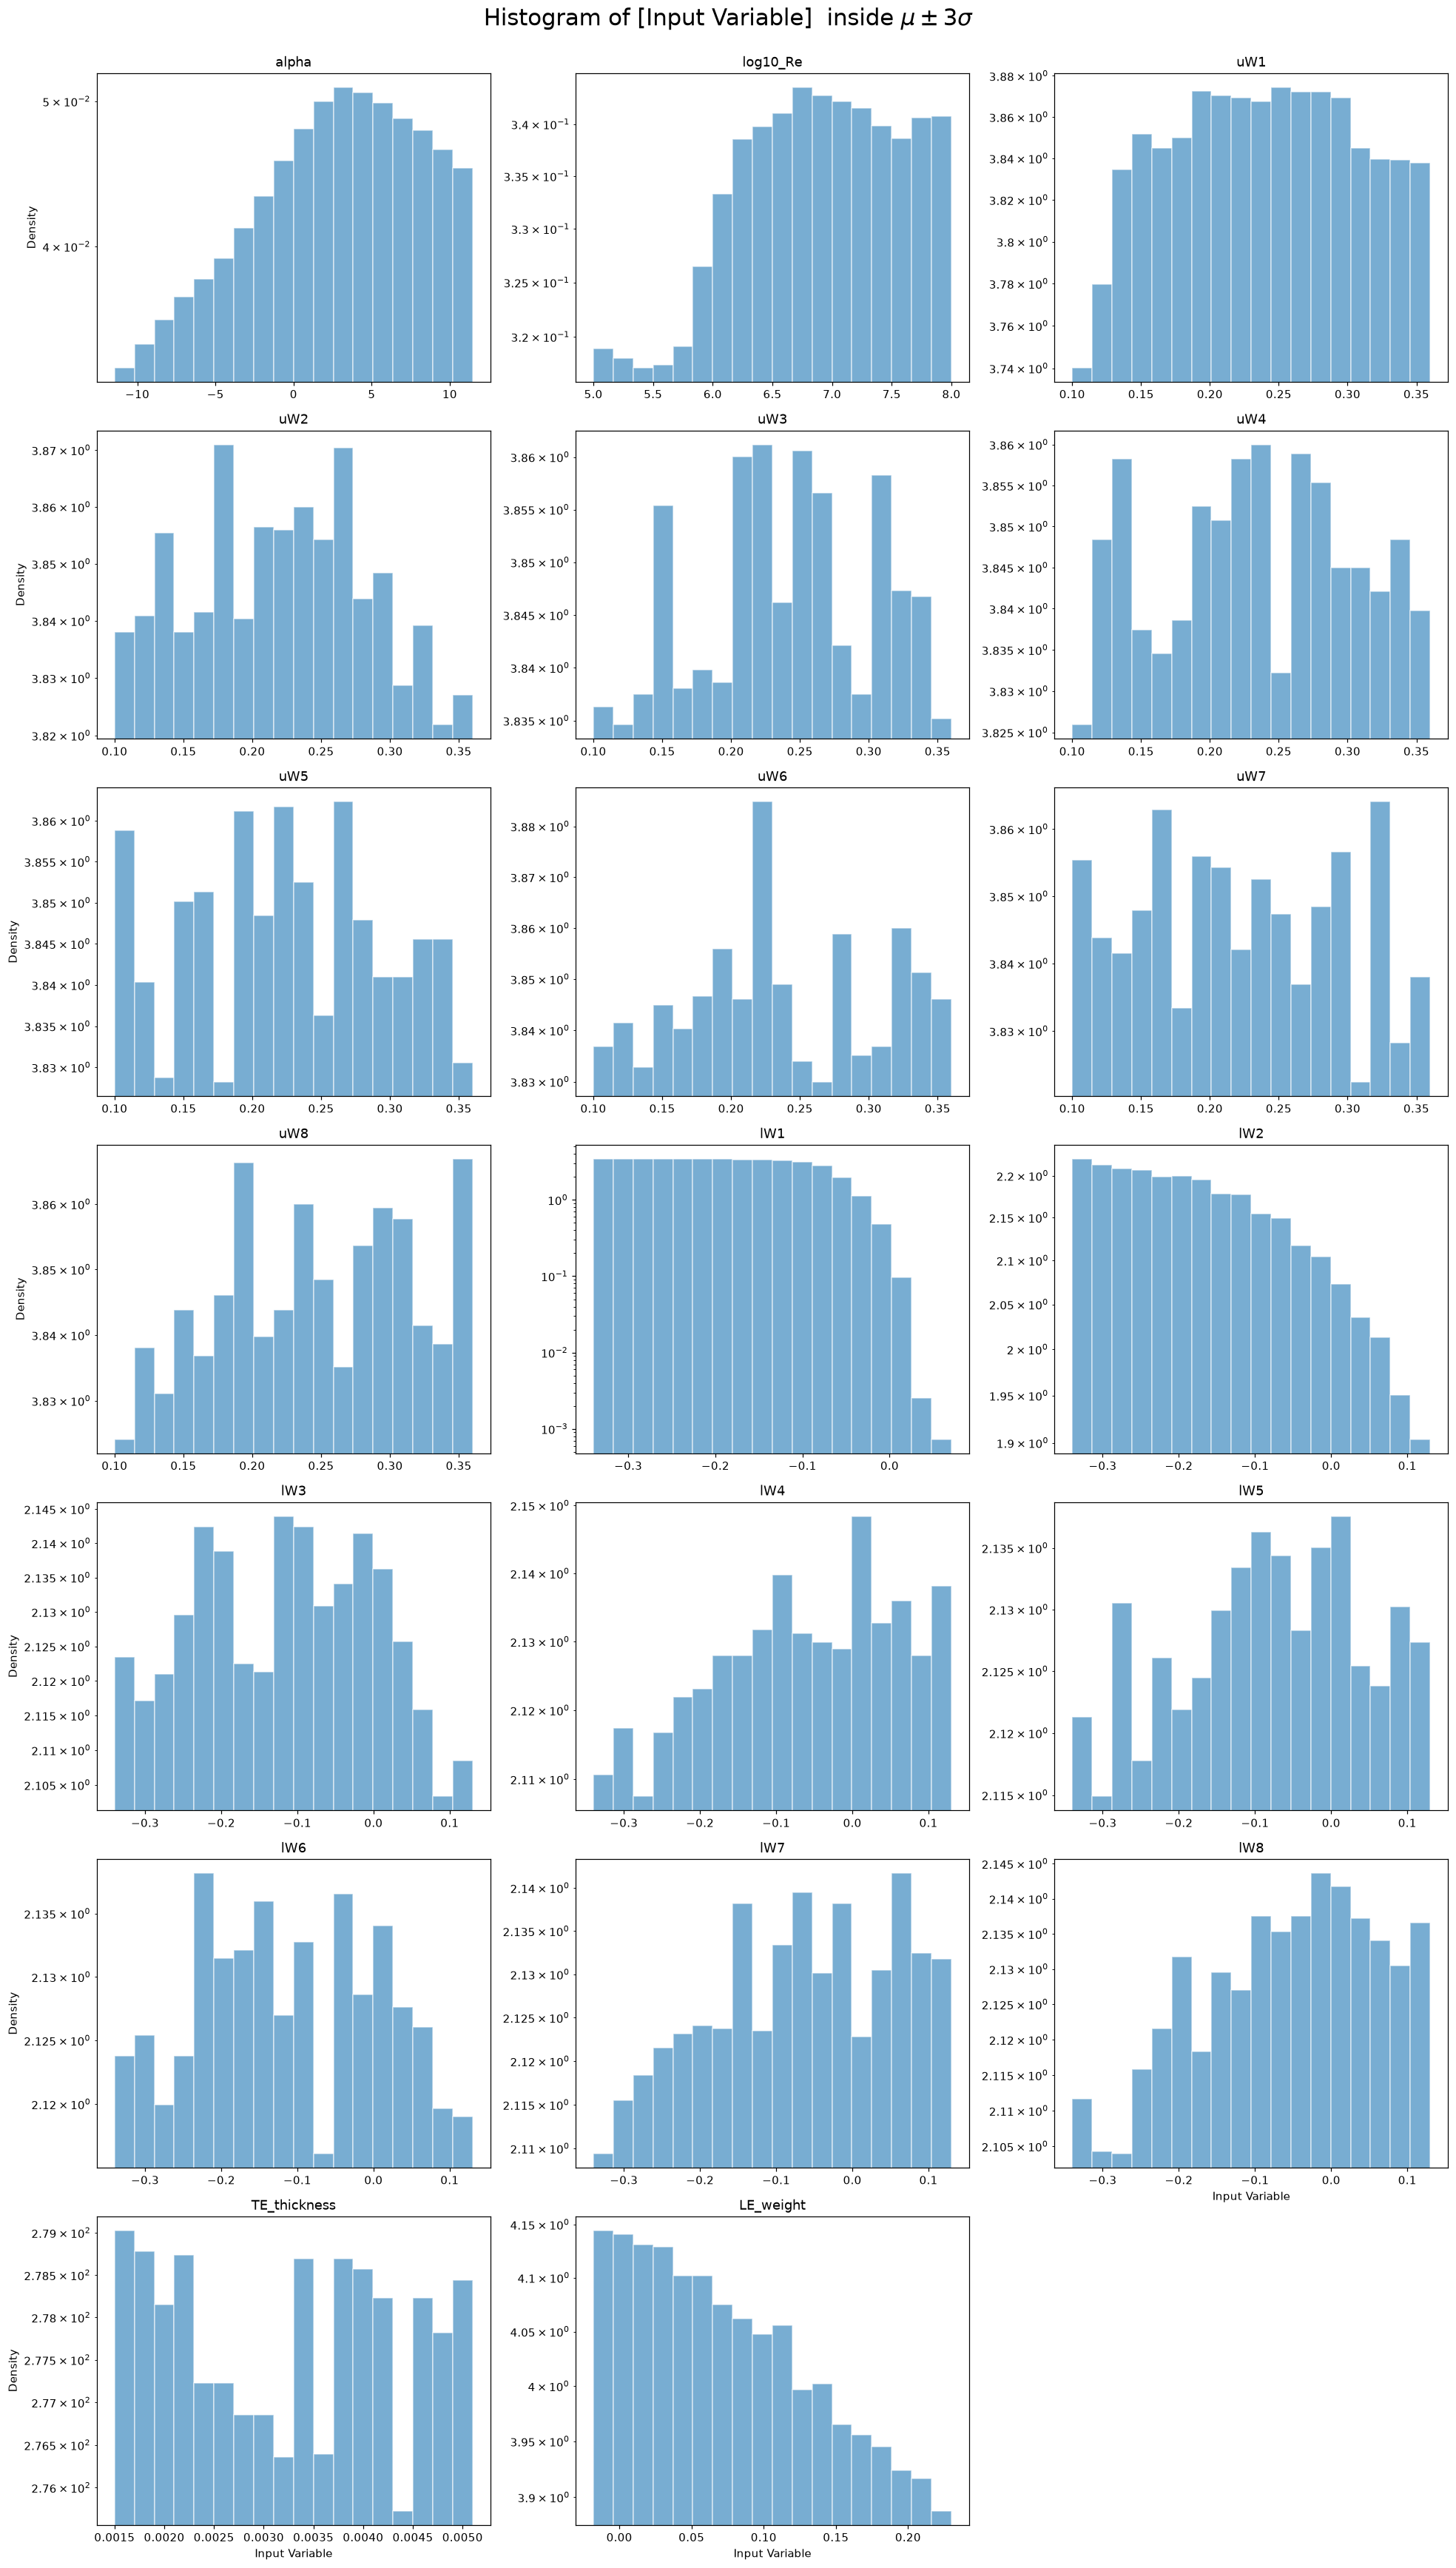
\includegraphics[width=1.0\linewidth,height=0.80\textheight,keepaspectratio]{analysis_plots/data_input_hist.png}\end{center}
\end{minipage}\par\medskip
\par\begin{minipage}{\linewidth}
\exhead{Input Cumulative Distributions}
\begin{center}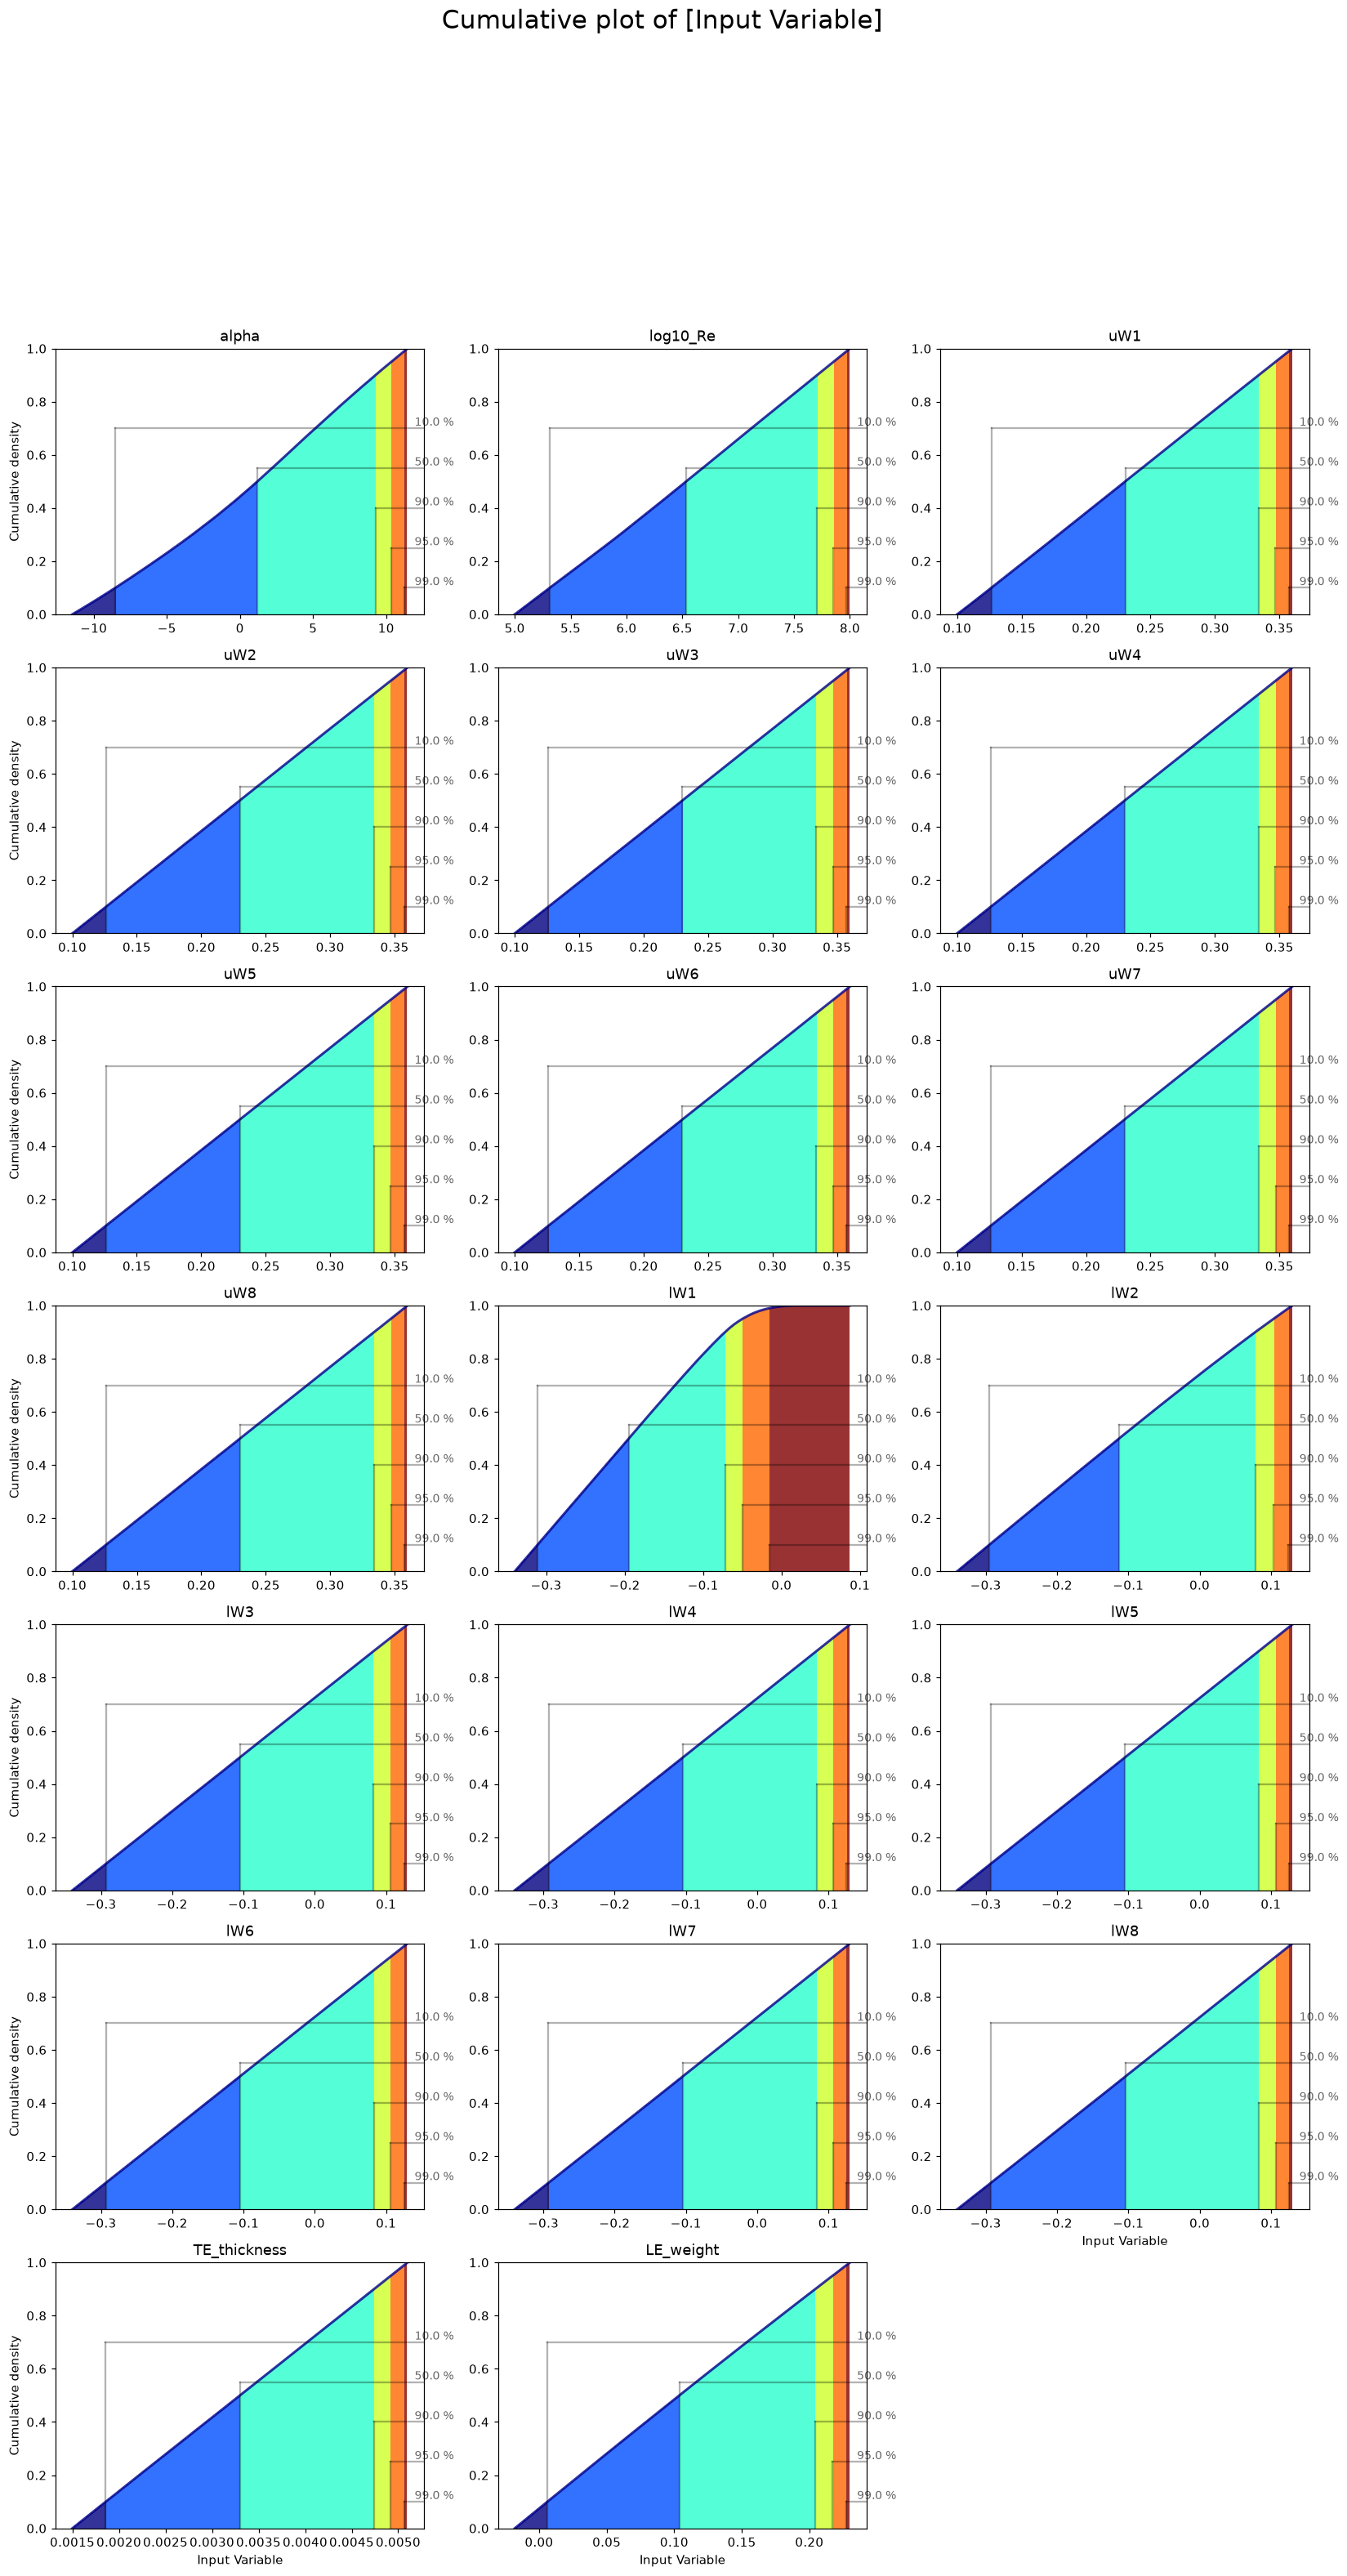
\includegraphics[width=1.0\linewidth,height=0.80\textheight,keepaspectratio]{analysis_plots/data_input_cdf.png}\end{center}
\end{minipage}\par\medskip
\exhead{Output Statistics}
\begin{center}
\footnotesize
\renewcommand{\arraystretch}{1.15}
\resizebox{\linewidth}{!}{%
\begin{tabular}{|l|r|r|r|r|r|r|r|r|}
\hline
\textbf{} & \textbf{count} & \textbf{mean} & \textbf{std} & \textbf{min} & \textbf{P25} & \textbf{P50} & \textbf{P75} & \textbf{max} \\ \hline
\textbf{CL} & 119,756 & 0.3298 & 0.7075 & -1.3751 & -0.2552 & 0.3931 & 0.9308 & 1.8332 \\ \hline
\textbf{CD} & 119,756 & 0.013 & 0.0134 & 0.0035 & 0.0068 & 0.0091 & 0.0141 & 0.1555 \\ \hline
\textbf{CM} & 119,756 & -0.0444 & 0.0341 & -0.182 & -0.0676 & -0.044 & -0.0209 & 0.0925 \\ \hline
\textbf{top\_transition\_location} & 119,756 & 0.3748 & 0.2965 & 0 & 0.1243 & 0.2911 & 0.6017 & 1 \\ \hline
\textbf{bottom\_transition\_location} & 119,756 & 0.3432 & 0.3408 & 0 & 0.0483 & 0.2009 & 0.6041 & 1 \\ \hline
\end{tabular}
}
\par\vspace{2pt}
{\scriptsize Output variables — Train\_set.describe()}
\end{center}
\par\begin{minipage}{\linewidth}
\exhead{Output Histograms}
\begin{center}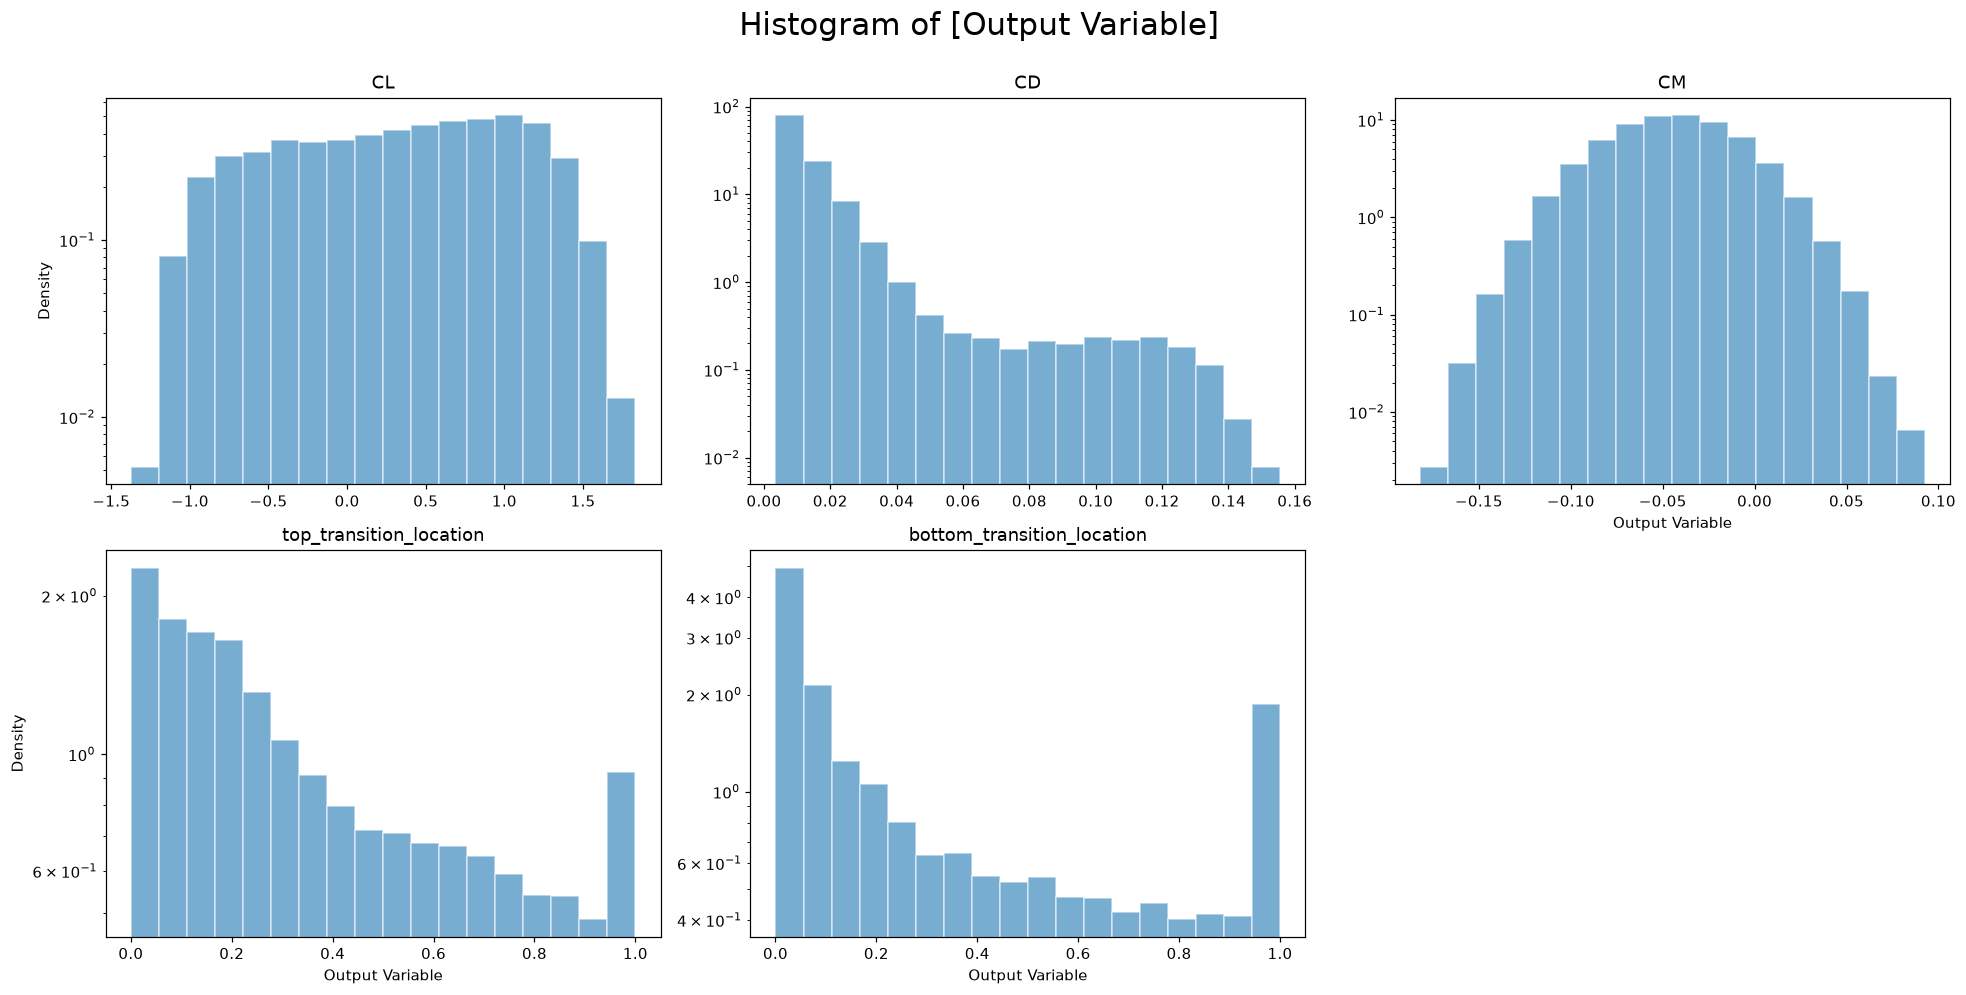
\includegraphics[width=1.0\linewidth,height=0.80\textheight,keepaspectratio]{analysis_plots/data_output_hist.png}\end{center}
\end{minipage}\par\medskip
\par\begin{minipage}{\linewidth}
\exhead{Output Cumulative Distributions}
\begin{center}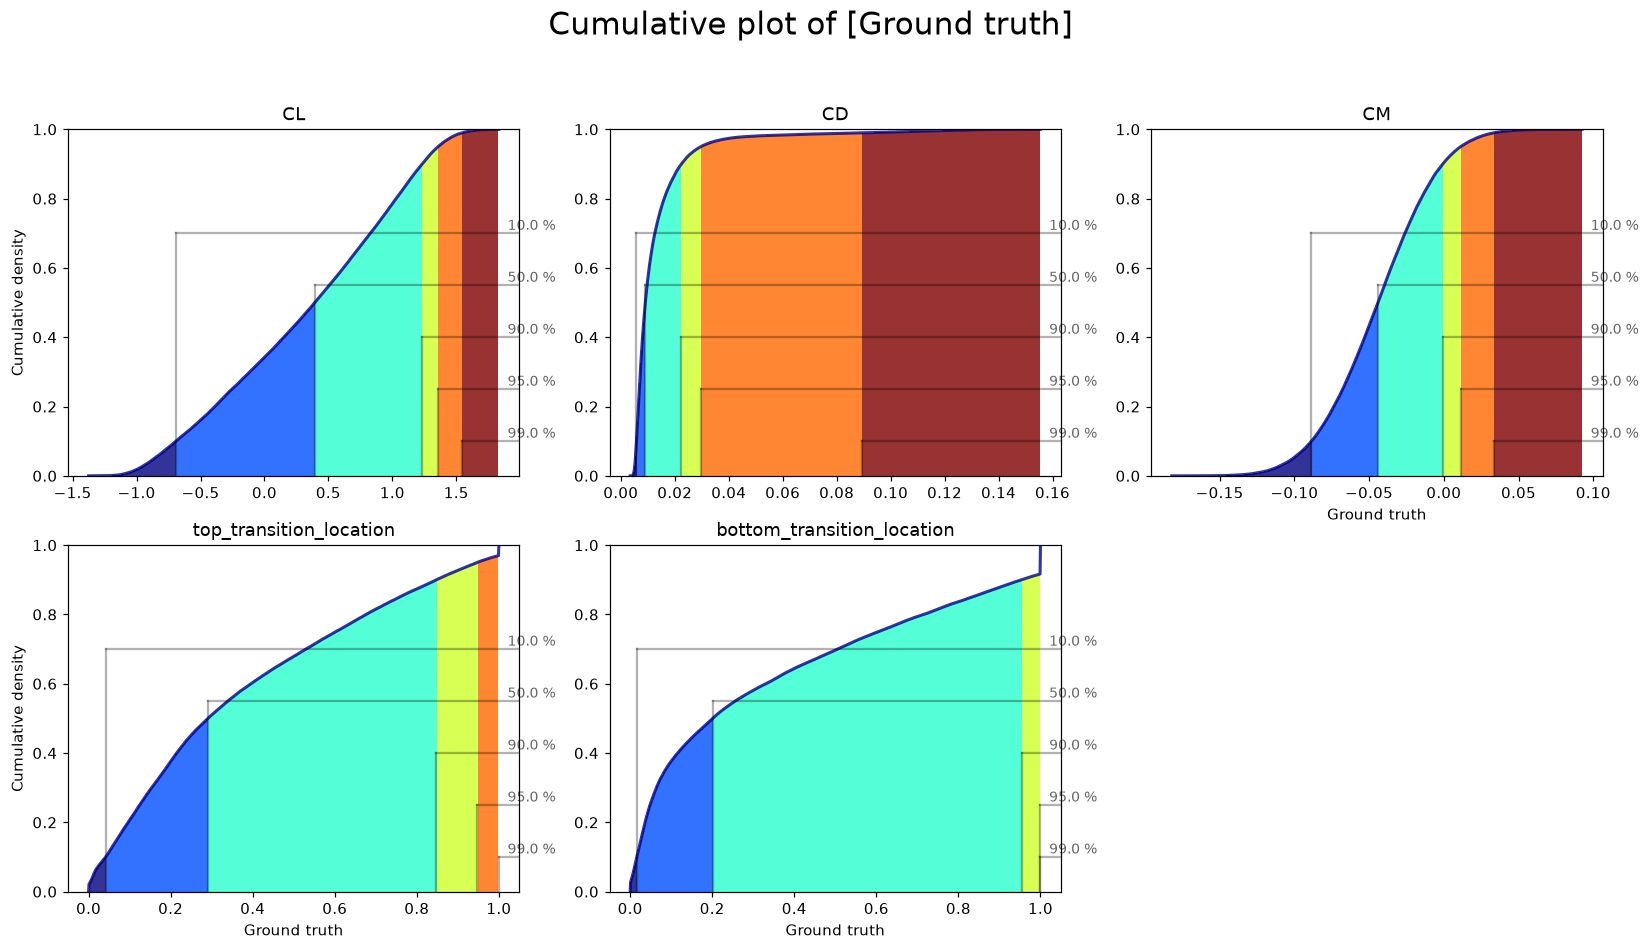
\includegraphics[width=1.0\linewidth,height=0.80\textheight,keepaspectratio]{analysis_plots/data_output_cdf.png}\end{center}
\end{minipage}\par\medskip
\clearpage
\section{Train-Test Split Analysis}
\label{sec:d2}

A well-designed split produces training and test distributions that are similar but not identical. The Kolmogorov-Smirnov (KS) test and the Anderson-Darling (AD) test are used to assess distributional similarity. $H_0$: both sets come from the same distribution. $p<0.05$ rejects $H_0$ (undesirable if too low; undesirable if the split was done by stratification and $p$ is too high).

\par\begin{minipage}{\linewidth}
\exhead{Output Distributions: Train vs Test}
\begin{center}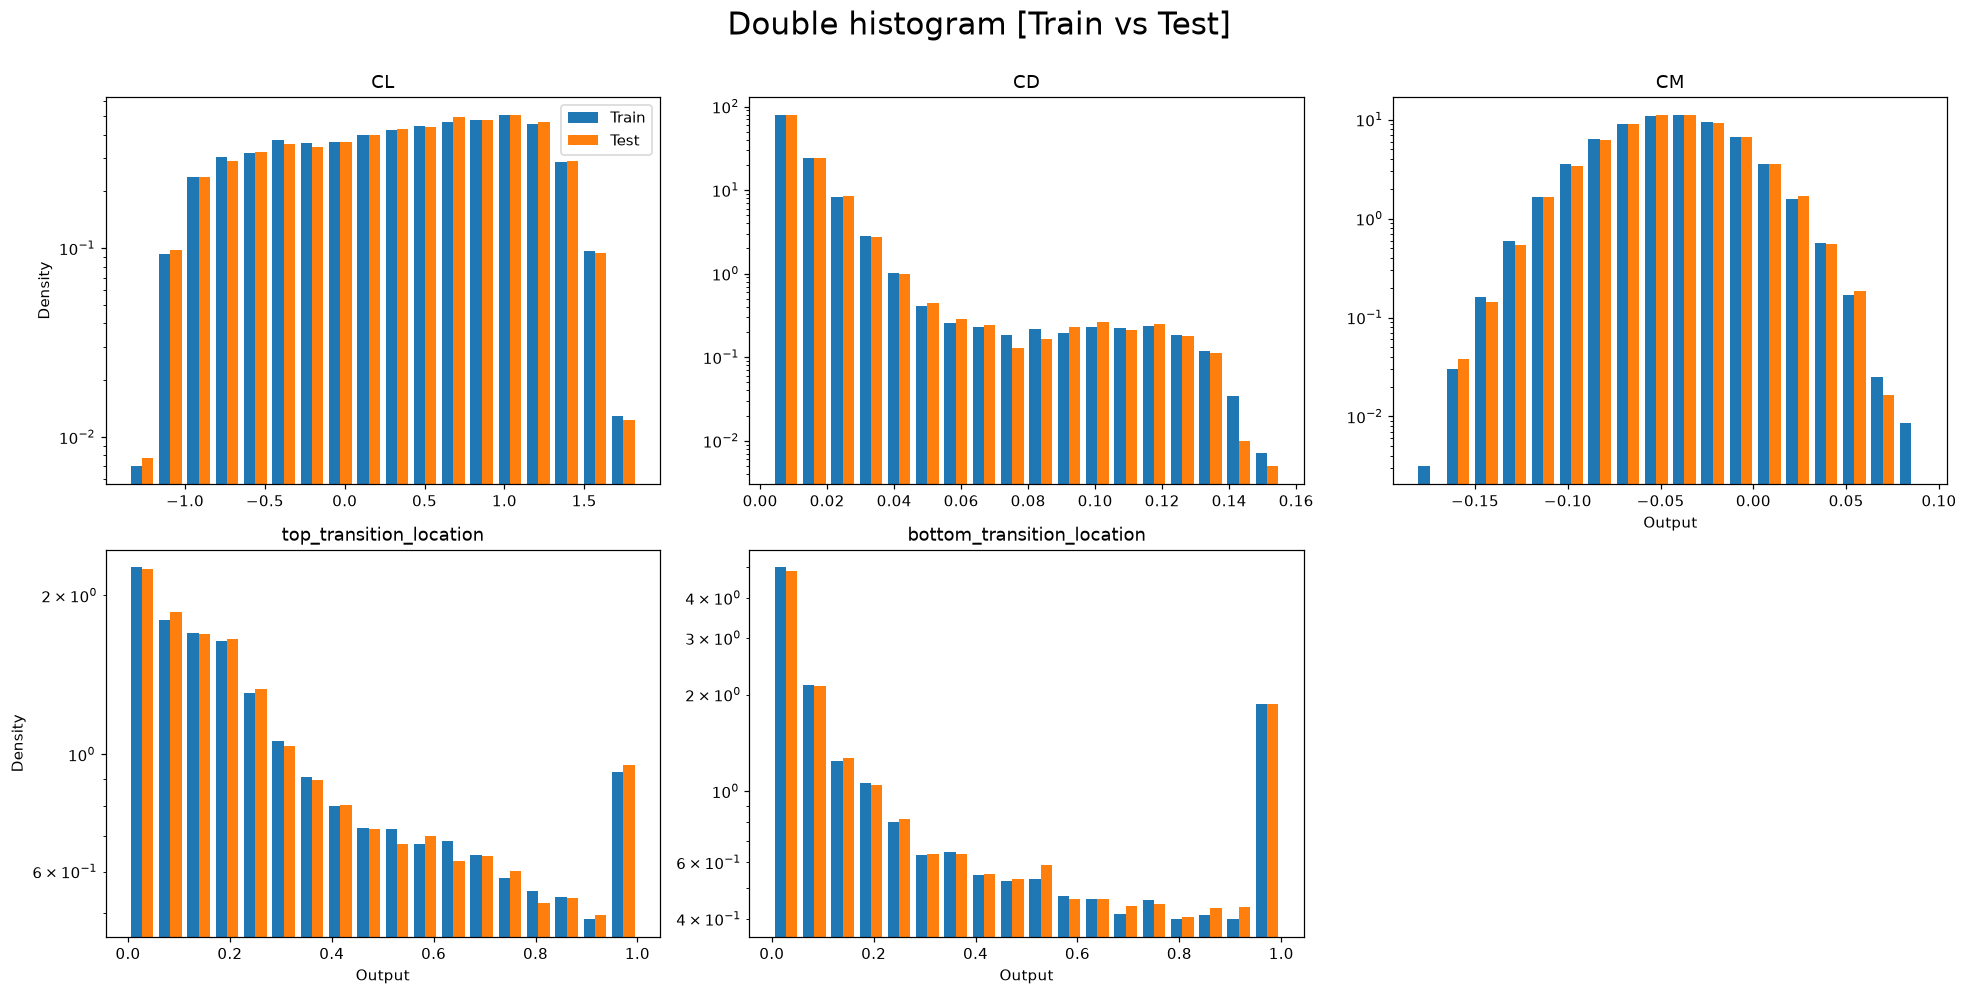
\includegraphics[width=1.0\linewidth,height=0.80\textheight,keepaspectratio]{analysis_plots/split_output_dists.png}\end{center}
\end{minipage}\par\medskip
\par\begin{minipage}{\linewidth}
\exhead{Input Distributions: Train vs Test}
\begin{center}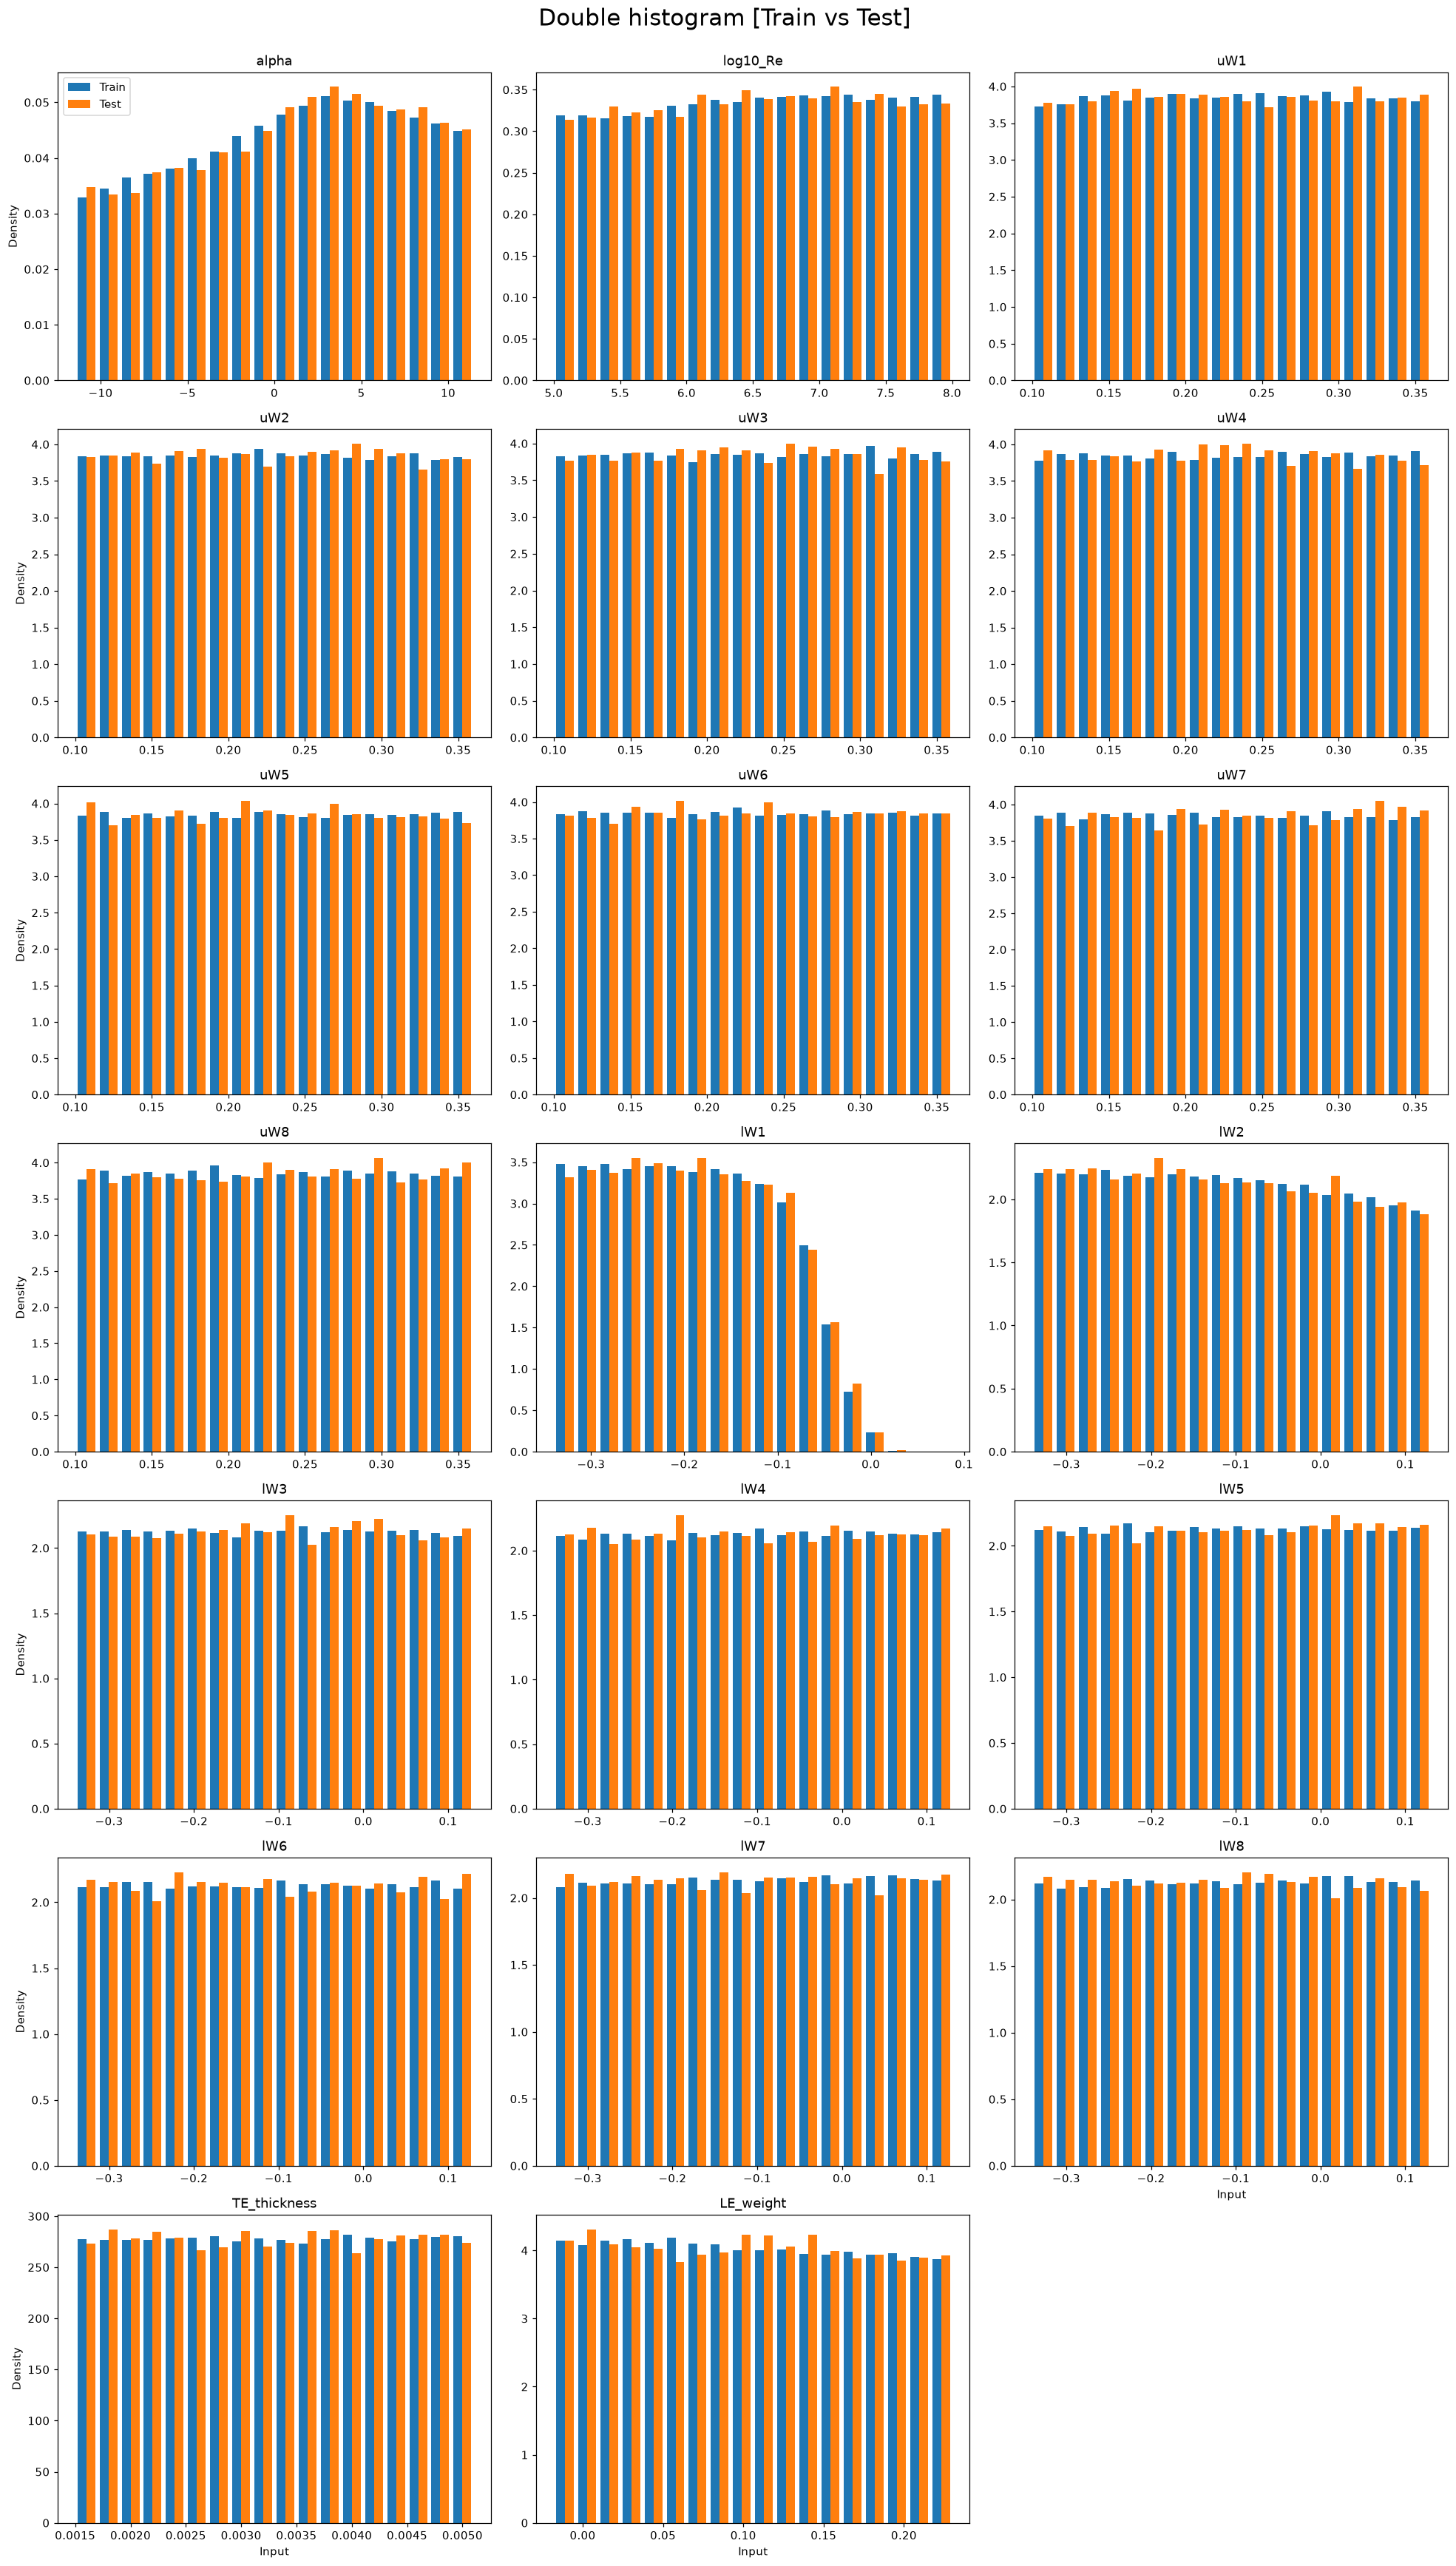
\includegraphics[width=1.0\linewidth,height=0.80\textheight,keepaspectratio]{analysis_plots/split_input_dists.png}\end{center}
\end{minipage}\par\medskip
\exhead{KS and AD Test Results}
\begin{center}
\footnotesize
\renewcommand{\arraystretch}{1.15}
\begin{tabular}{|l|r|r|}
\hline
\textbf{} & \textbf{KS} & \textbf{AD} \\ \hline
\textbf{CL} & \cellcolor{passgreen}0.0905 & \cellcolor{passgreen}0.1513 \\ \hline
\textbf{CD} & \cellcolor{passgreen}0.3411 & \cellcolor{passgreen}0.25 \\ \hline
\textbf{CM} & \cellcolor{passgreen}0.3781 & \cellcolor{passgreen}0.25 \\ \hline
\textbf{top\_transition\_location} & \cellcolor{passgreen}0.5412 & \cellcolor{passgreen}0.25 \\ \hline
\textbf{bottom\_transition\_location} & \cellcolor{passgreen}0.0754 & \cellcolor{failred}0.0371 \\ \hline
\end{tabular}
\par\vspace{2pt}
{\scriptsize Train vs test p-values. Red: $p<0.05$ (distributions differ).}
\end{center}
\exhead{Split Quality --- Voxel Tesselation Proximity (p-hacking check)}
Beyond matching distributions, a split can still flatter the model if test points sit right next to training points (\textbf{p-hacking}) or probe regions the model never saw (\textbf{isolated}, \textbf{residual voxel}). The VTPM method from \texttt{validationlib} (SF\_9 cell 9.0) classifies every test point.

\begin{minipage}{\linewidth}
\renewcommand{\arraystretch}{1.2}
\begin{tabular}{|l|r|c|}
  \hline\textbf{Metric} & \textbf{Value} & \textbf{Pass} \\ \hline
  Residual voxel proportion ($\leq\!0.05$) & 0.000 & \cellcolor{passgreen}$\checkmark$ \\ \hline
  Valid test proportion & 0.965 & \\ \hline
  p-hacking test proportion ($\leq\!0.05$ warn) & 0.003 & \cellcolor{passgreen}$\checkmark$ \\ \hline
  Isolated test proportion ($\leq\!0.05$ warn) & 0.033 & \cellcolor{passgreen}$\checkmark$ \\ \hline
  Chi\textsuperscript{2} p-value ($\geq\!0.05$) & \textemdash & \textemdash \\ \hline
\end{tabular}
\end{minipage}

\textcolor{passgreen!60!black}{\textbf{No p-hacking concern:}} only 0.2\% of test points lie closer to a training point than training points are to each other, so the test error is not flattered.

\par\begin{minipage}{\linewidth}
\exhead{Error Distribution: Valid vs Isolated Test Points}
Same comparison for the test points with no training neighbour.
\begin{center}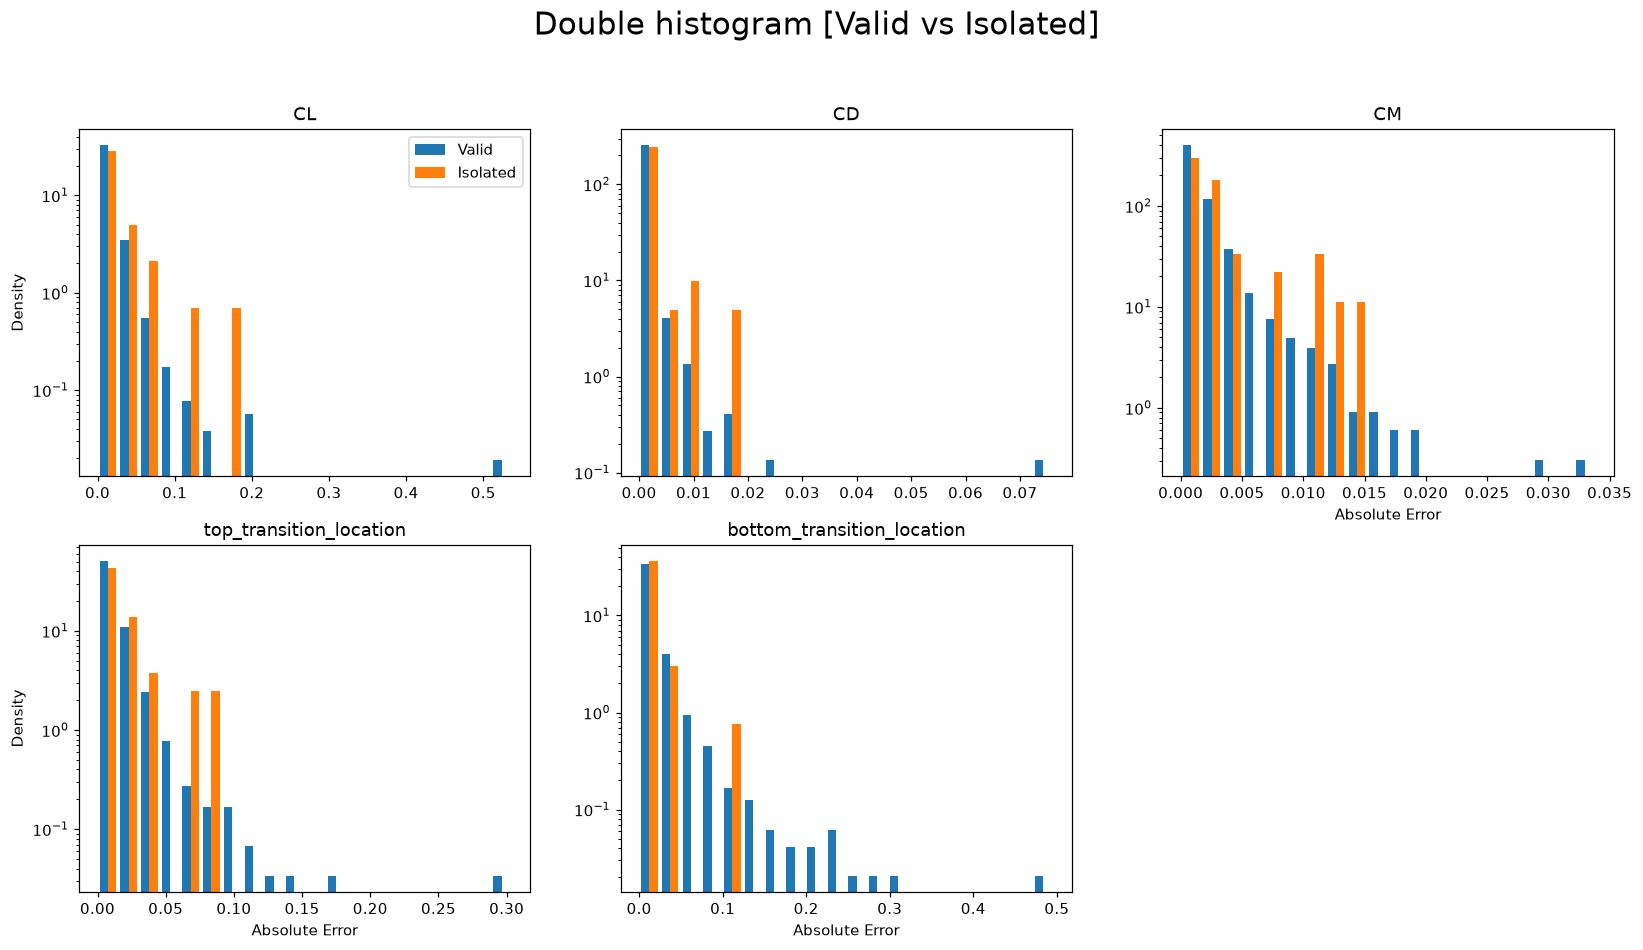
\includegraphics[width=1.0\linewidth,height=0.80\textheight,keepaspectratio]{analysis_plots/isolated_hist.png}\end{center}
\begin{center}
\footnotesize
\renewcommand{\arraystretch}{1.15}
\begin{tabular}{|l|r|r|r|}
\hline
\textbf{} & \textbf{AD} & \textbf{KS} & \textbf{KW} \\ \hline
\textbf{CL} & \cellcolor{failred}0.0256 & \cellcolor{passgreen}0.0581 & \cellcolor{failred}0.0358 \\ \hline
\textbf{CD} & \cellcolor{failred}0.0034 & \cellcolor{failred}0.0327 & \cellcolor{failred}0.0142 \\ \hline
\textbf{CM} & \cellcolor{failred}0.0156 & \cellcolor{failred}0.0111 & \cellcolor{failred}0.0405 \\ \hline
\textbf{top\_transition\_location} & \cellcolor{passgreen}0.1573 & \cellcolor{passgreen}0.3304 & \cellcolor{passgreen}0.2561 \\ \hline
\textbf{bottom\_transition\_location} & \cellcolor{passgreen}0.25 & \cellcolor{passgreen}0.657 & \cellcolor{passgreen}0.3696 \\ \hline
\end{tabular}
\par\vspace{2pt}
{\scriptsize Valid ($n=1946$) vs Isolated ($n=53$) absolute-error distributions, on a subsample of the test set. Red: $p<0.05$ (the flagged points behave differently).}
\end{center}
\end{minipage}\par\medskip
\clearpage
\section{Error Quantification --- P(E)}
\label{sec:d3}

Two error metrics are studied:
\begin{itemize}[leftmargin=1.4em,itemsep=1pt,topsep=1pt]
  \item \textbf{Residue:} $e_i = y_i - \hat{y}_i$. A centred ($\mu\approx 0$), symmetric distribution indicates an unbiased model.
  \item \textbf{Absolute Error:} $|e_i|$. Always non-negative; its Q90 must satisfy the accuracy requirement.
\end{itemize}

\exhead{Residue Statistics Table}
Bootstrap confidence bounds shown as superscript (upper) and subscript (lower).
\begin{center}
\footnotesize
\renewcommand{\arraystretch}{1.15}
\resizebox{\linewidth}{!}{%
\begin{tabular}{|l|r|r|r|r|r|r|r|r|r|r|r|r|r|r|r|}
\hline
\textbf{} & \textbf{count} & \textbf{min} & \textbf{max} & \textbf{mean} & \textbf{(BS)mean} & \textbf{median} & \textbf{(BS)median} & \textbf{std} & \textbf{(BS)std} & \textbf{IQR} & \textbf{(BS)IQR} & \textbf{kurtosis} & \textbf{(BS)kurtosis} & \textbf{skewness} & \textbf{(BS)skewness} \\ \hline
\textbf{CL} & 23,952 & -0.363 & 0.537 & -0.000348 & $^{\text{-5.25e-05}}_{-0.000682}$ & -0.0012 & $^{-0.000964}_{-0.0015}$ & 0.0249 & $^{0.0261}_{0.0236}$ & 0.0213 & $^{0.0216}_{0.0209}$ & 54.4 & $^{75.5}_{34.7}$ & 2.21 & $^{3.59}_{0.835}$ \\ \hline
\textbf{CD} & 23,952 & -0.0661 & 0.0762 & -1.37e-05 & $^{\text{1.28e-05}}_{\text{-3.88e-05}}$ & -6.26e-06 & $^{\text{-2.47e-06}}_{\text{-9.88e-06}}$ & 0.0022 & $^{0.0024}_{0.0019}$ & 0.000346 & $^{0.000352}_{0.000339}$ & 307 & $^{389}_{208}$ & 5.98 & $^{10.8}_{0.254}$ \\ \hline
\textbf{CM} & 23,952 & -0.0296 & 0.0395 & -0.000119 & $^{\text{-8.38e-05}}_{-0.000159}$ & -0.000183 & $^{-0.000157}_{-0.000206}$ & 0.0031 & $^{0.0031}_{0.003}$ & 0.0022 & $^{0.0022}_{0.0022}$ & 17 & $^{20.3}_{14}$ & 1.04 & $^{1.42}_{0.69}$ \\ \hline
\textbf{top\_transition\_location} & 23,952 & -0.304 & 0.211 & 0.0028 & $^{0.0029}_{0.0025}$ & 0.0018 & $^{0.002}_{0.0016}$ & 0.0178 & $^{0.0183}_{0.0174}$ & 0.0152 & $^{0.0154}_{0.015}$ & 20.3 & $^{26.3}_{15.1}$ & 0.0865 & $^{0.61}_{-0.581}$ \\ \hline
\textbf{bottom\_transition\_location} & 23,952 & -0.496 & 0.428 & -0.0053 & $^{-0.0051}_{-0.0057}$ & -0.0053 & $^{-0.0052}_{-0.0055}$ & 0.0278 & $^{0.0284}_{0.0265}$ & 0.016 & $^{0.0162}_{0.0157}$ & 33.7 & $^{41.6}_{26.5}$ & 0.483 & $^{1.16}_{-0.163}$ \\ \hline
\end{tabular}
}
\par\vspace{2pt}
{\scriptsize Residue statistics with bootstrap confidence intervals (superscript/subscript bounds).}
\end{center}
\exhead{Absolute Error Statistics Table}
\begin{center}
\footnotesize
\renewcommand{\arraystretch}{1.15}
\resizebox{\linewidth}{!}{%
\begin{tabular}{|l|r|r|r|r|r|r|r|r|r|r|r|r|r|r|r|}
\hline
\textbf{} & \textbf{count} & \textbf{min} & \textbf{max} & \textbf{mean} & \textbf{(BS)mean} & \textbf{median} & \textbf{(BS)median} & \textbf{std} & \textbf{(BS)std} & \textbf{IQR} & \textbf{(BS)IQR} & \textbf{kurtosis} & \textbf{(BS)kurtosis} & \textbf{skewness} & \textbf{(BS)skewness} \\ \hline
\textbf{CL} & 23,952 & 1.28e-06 & 0.537 & 0.0153 & $^{0.0155}_{0.0151}$ & 0.0106 & $^{0.0108}_{0.0104}$ & 0.0196 & $^{0.021}_{0.0181}$ & 0.0143 & $^{0.0146}_{0.0141}$ & 118 & $^{153}_{67}$ & 7.55 & $^{8.92}_{5.78}$ \\ \hline
\textbf{CD} & 23,952 & 1.09e-08 & 0.0762 & 0.000577 & $^{0.000599}_{0.00055}$ & 0.00017 & $^{0.000174}_{0.000167}$ & 0.0021 & $^{0.0023}_{0.0018}$ & 0.000343 & $^{0.000352}_{0.000336}$ & 339 & $^{437}_{231}$ & 15.1 & $^{17.1}_{12.6}$ \\ \hline
\textbf{CM} & 23,952 & 1.46e-07 & 0.0395 & 0.0018 & $^{0.0019}_{0.0018}$ & 0.0011 & $^{0.0011}_{0.0011}$ & 0.0024 & $^{0.0025}_{0.0024}$ & 0.0016 & $^{0.0017}_{0.0016}$ & 29 & $^{34.6}_{24.1}$ & 4.23 & $^{4.58}_{3.94}$ \\ \hline
\textbf{top\_transition\_location} & 23,952 & 1.01e-06 & 0.304 & 0.0114 & $^{0.0115}_{0.0112}$ & 0.0076 & $^{0.0077}_{0.0075}$ & 0.0139 & $^{0.0144}_{0.0134}$ & 0.011 & $^{0.0112}_{0.0108}$ & 39.9 & $^{55.3}_{29.4}$ & 4.61 & $^{5.22}_{4.11}$ \\ \hline
\textbf{bottom\_transition\_location} & 23,952 & 1.47e-07 & 0.496 & 0.0157 & $^{0.016}_{0.0154}$ & 0.0093 & $^{0.0094}_{0.0091}$ & 0.0236 & $^{0.0245}_{0.0226}$ & 0.0136 & $^{0.0139}_{0.0133}$ & 50.1 & $^{61.2}_{39}$ & 5.58 & $^{6.04}_{5.04}$ \\ \hline
\end{tabular}
}
\par\vspace{2pt}
{\scriptsize Absolute-error statistics with bootstrap confidence intervals.}
\end{center}
\par\begin{minipage}{\linewidth}
\exhead{Residue Histograms}
\begin{center}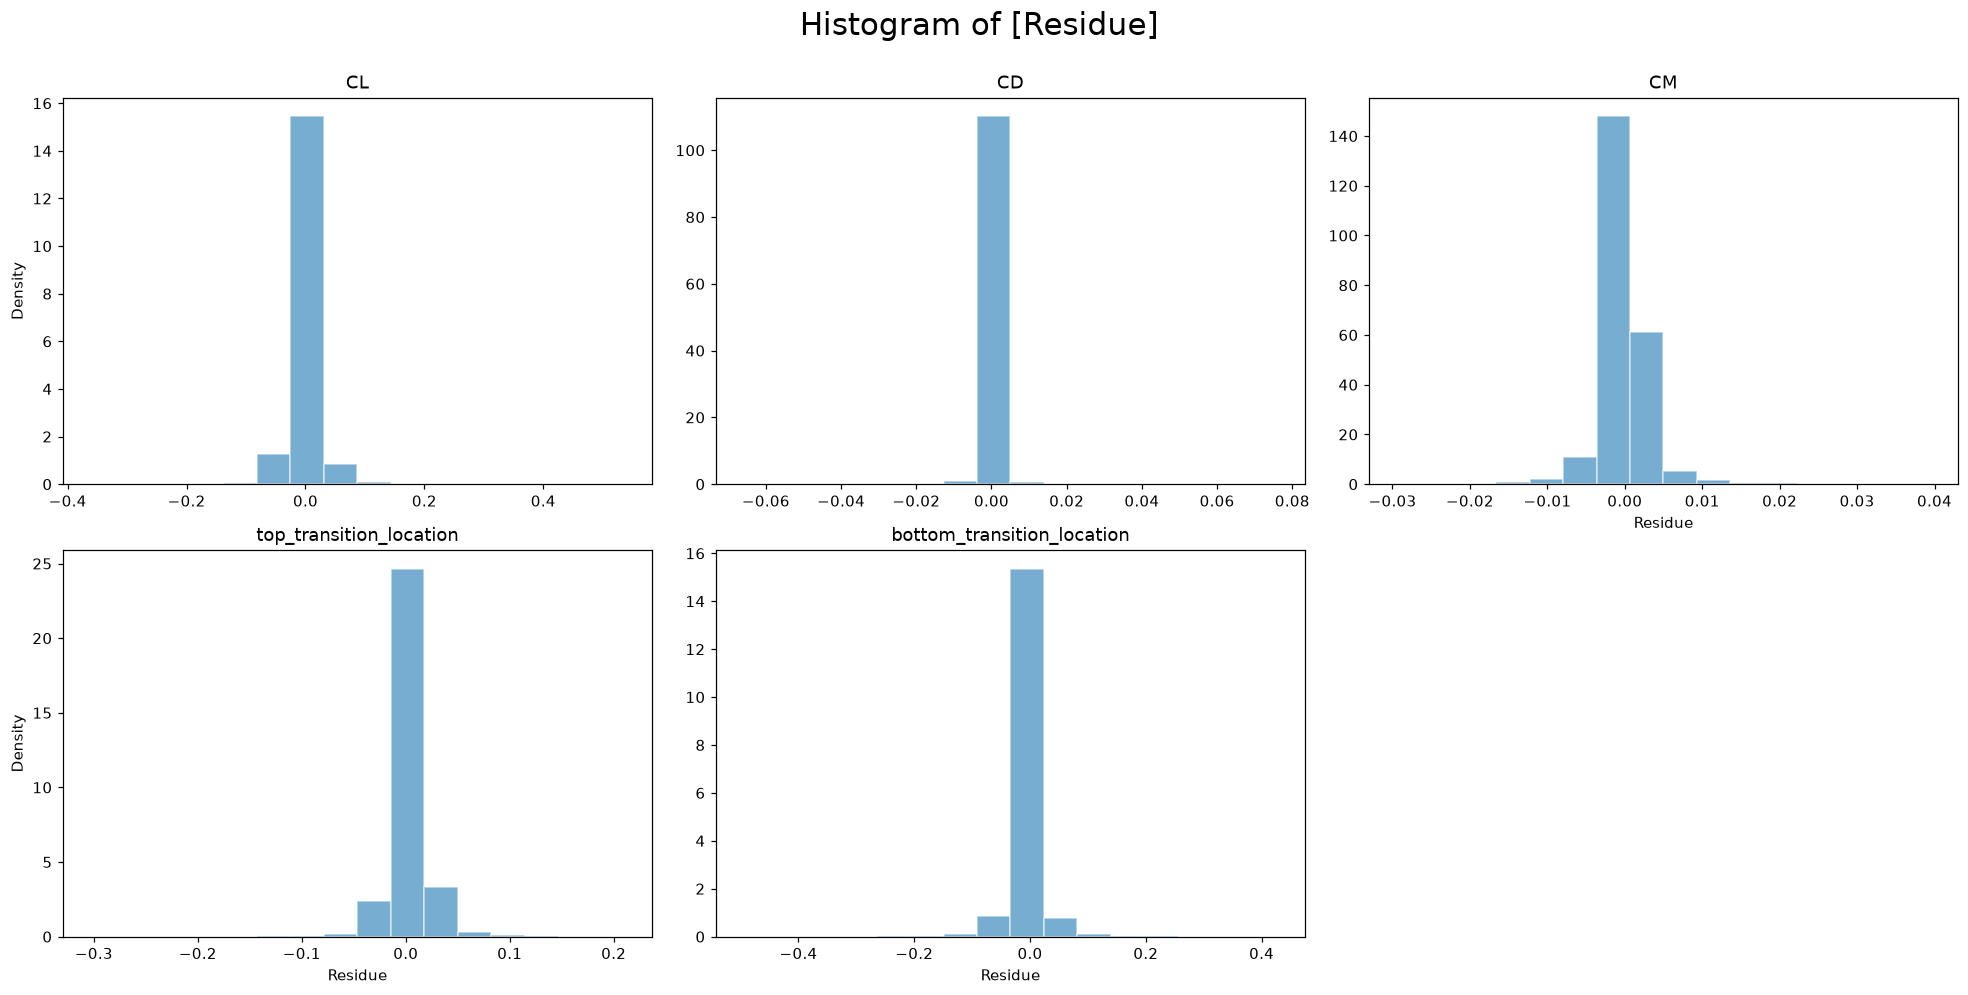
\includegraphics[width=1.0\linewidth,height=0.80\textheight,keepaspectratio]{analysis_plots/err_residue_hist.png}\end{center}
\end{minipage}\par\medskip
\par\begin{minipage}{\linewidth}
\exhead{Residue CDF}
\begin{center}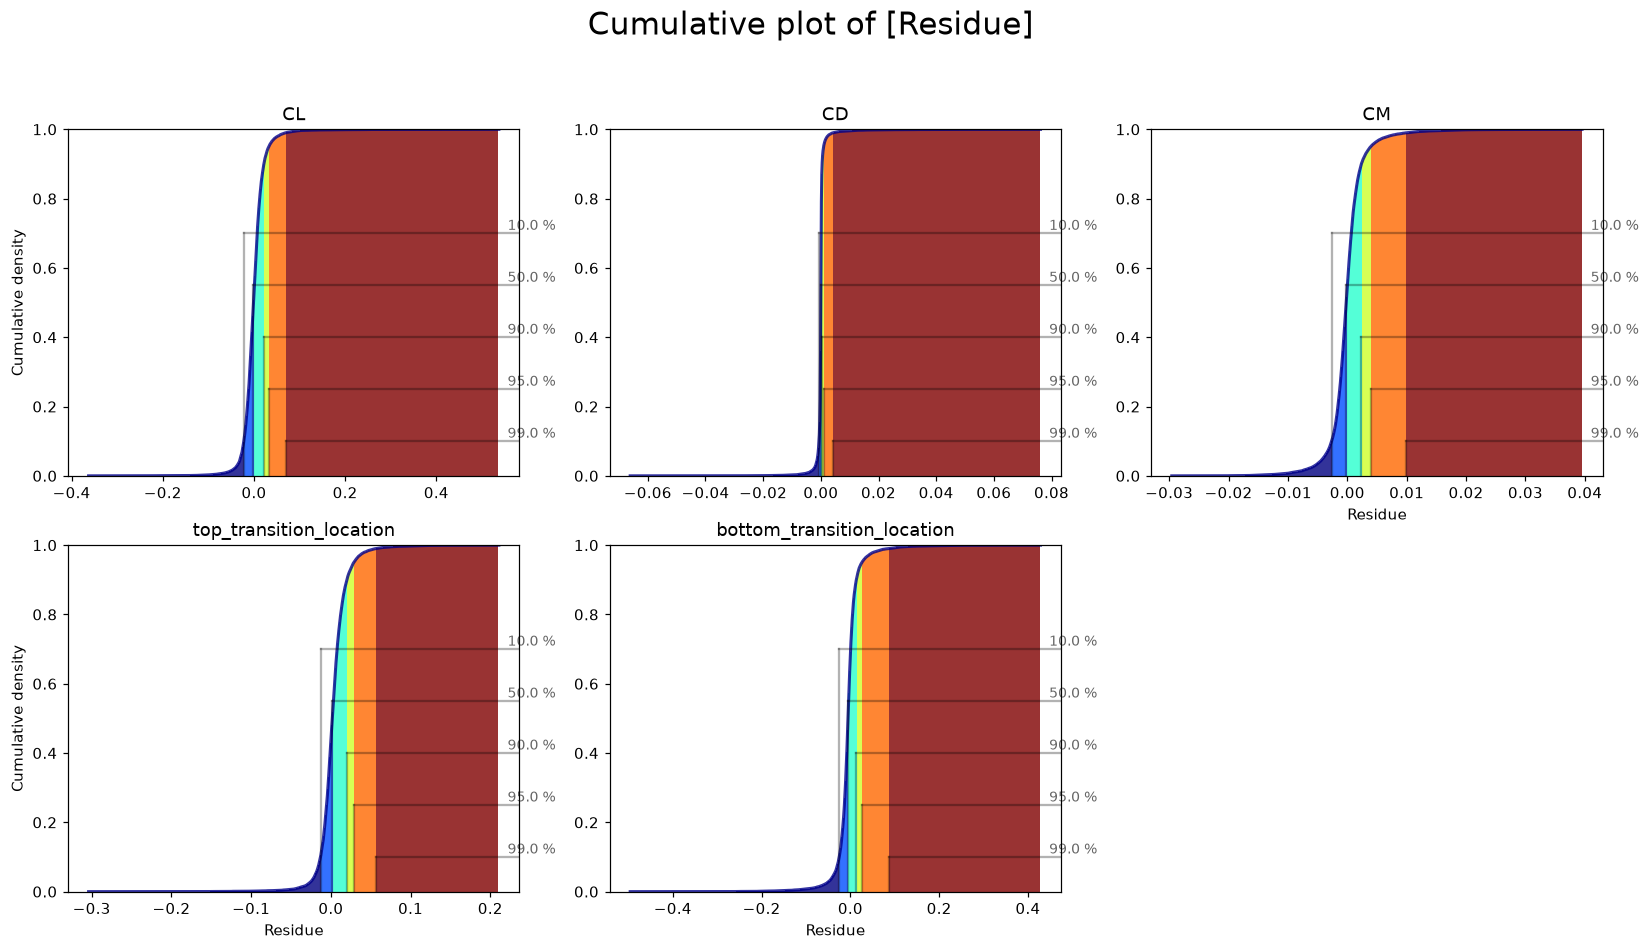
\includegraphics[width=1.0\linewidth,height=0.80\textheight,keepaspectratio]{analysis_plots/err_residue_cdf.png}\end{center}
\end{minipage}\par\medskip
\par\begin{minipage}{\linewidth}
\exhead{Absolute Error Histograms}
\begin{center}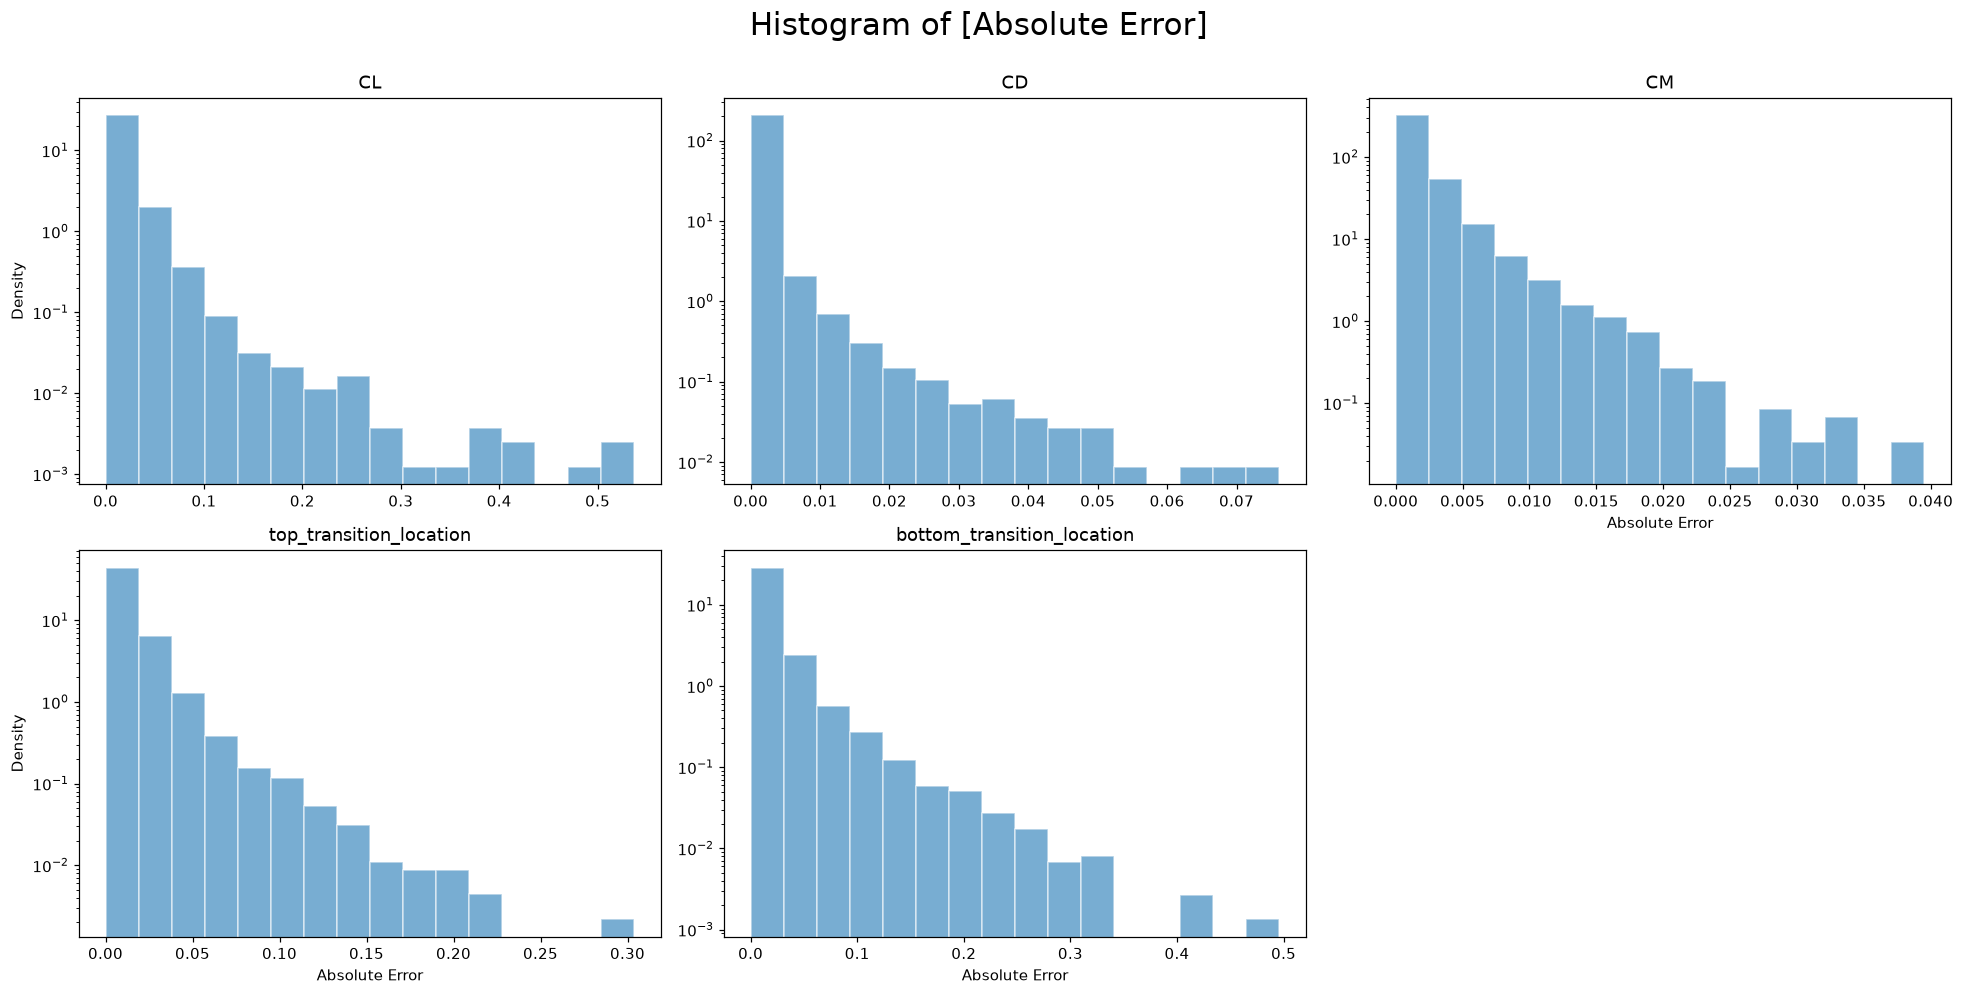
\includegraphics[width=1.0\linewidth,height=0.80\textheight,keepaspectratio]{analysis_plots/err_abserr_hist.png}\end{center}
\end{minipage}\par\medskip
\exhead{Q90 Accuracy Requirement}
\begin{minipage}{\linewidth}
\renewcommand{\arraystretch}{1.2}
\begin{tabular}{|l|r|r|c|}
  \hline\textbf{Output} & \textbf{Q90} & \textbf{Target} & \textbf{Status} \\ \hline
  CL & \cellcolor{failred}0.1107 & 10\% & \cellcolor{failred}\textbf{FAIL} \\ \hline
  CD & \cellcolor{passgreen}0.0632 & 10\% & \cellcolor{passgreen}\textbf{PASS} \\ \hline
  CM & \cellcolor{failred}0.2174 & 10\% & \cellcolor{failred}\textbf{FAIL} \\ \hline
  top\_transition\_location & \cellcolor{failred}0.1554 & 10\% & \cellcolor{failred}\textbf{FAIL} \\ \hline
  bottom\_transition\_location & \cellcolor{failred}0.3584 & 10\% & \cellcolor{failred}\textbf{FAIL} \\ \hline
\end{tabular}
\par\vspace{4pt}
{\footnotesize \colorbox{passgreen}{\ } $p\geq 0.05$ --- pass\enspace \colorbox{failred}{\ } $p<0.05$ --- fail}
\end{minipage}

\par\begin{minipage}{\linewidth}
\exhead{True vs Predicted Distribution Comparison}
AD and KS tests comparing the distribution of true vs.\ predicted values on the test set. A significant difference indicates the model is not reproducing the output distribution faithfully.
\begin{center}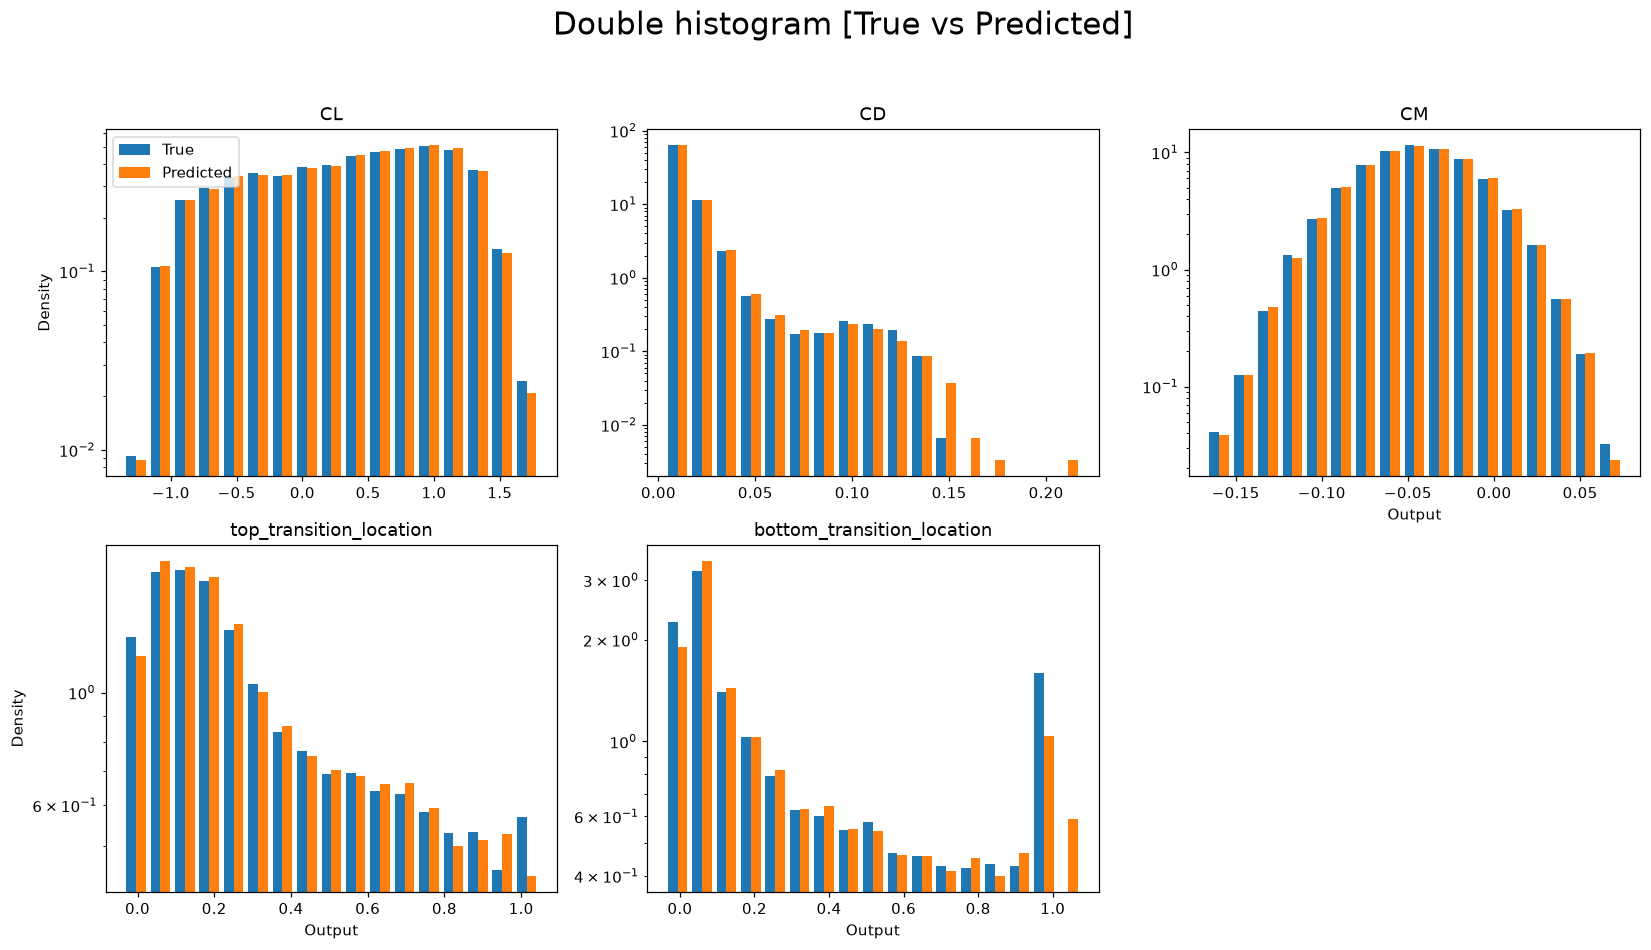
\includegraphics[width=1.0\linewidth,height=0.80\textheight,keepaspectratio]{analysis_plots/err_true_vs_pred_dist.png}\end{center}
\begin{center}
\footnotesize
\renewcommand{\arraystretch}{1.15}
\begin{tabular}{|l|r|r|}
\hline
\textbf{} & \textbf{AD} & \textbf{KS} \\ \hline
\textbf{CL} & \cellcolor{passgreen}0.25 & \cellcolor{passgreen}0.9942 \\ \hline
\textbf{CD} & \cellcolor{passgreen}0.25 & \cellcolor{passgreen}0.9957 \\ \hline
\textbf{CM} & \cellcolor{passgreen}0.25 & \cellcolor{passgreen}0.9671 \\ \hline
\textbf{top\_transition\_location} & \cellcolor{failred}0.0014 & \cellcolor{failred}0.000816 \\ \hline
\textbf{bottom\_transition\_location} & \cellcolor{failred}0.001 & \cellcolor{failred}3.9e-37 \\ \hline
\end{tabular}
\par\vspace{2pt}
{\scriptsize True vs predicted distribution tests. Red: $p<0.05$.}
\end{center}
\end{minipage}\par\medskip
\par\begin{minipage}{\linewidth}
\exhead{True vs Predicted --- 2D Histogram}
Log-scaled frequency with a linear fit; the normalized slope should be close to 1.
\begin{center}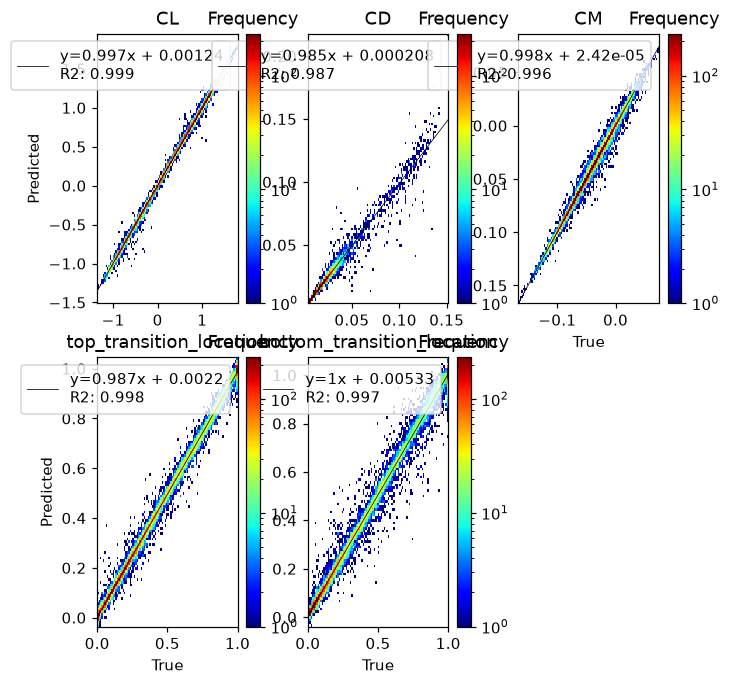
\includegraphics[width=1.0\linewidth,height=0.80\textheight,keepaspectratio]{analysis_plots/true_pred_hist2d.png}\end{center}
\end{minipage}\par\medskip
\clearpage
\section{P(E|X) --- Error Conditional on Inputs}
\label{sec:d4}

We study whether the model error depends on the input variables. Two approaches are used: (1) a Kruskal-Wallis (KW) test on binned inputs (Sturges rule for bin count), and (2) violin plots showing the error distribution within each input bin.

Significant input-conditional bias ($p<0.05$) detected for: \textcolor{red}{\textit{alpha$\to$CL, alpha$\to$CD, alpha$\to$CM, alpha$\to$top\_transition\_location, alpha$\to$bottom\_transition\_location, log10\_Re$\to$CL, log10\_Re$\to$CD, log10\_Re$\to$CM, log10\_Re$\to$top\_transition\_location, log10\_Re$\to$bottom\_transition\_location\ldots}}. These inputs explain residual variance --- consider polynomial features or interaction terms.

\exhead{Bias Detection Table (KW p-values)}
Green ($p\geq 0.05$) = residue uniform across input bins; red ($p<0.05$) = significant bias.
\begin{center}
\footnotesize
\renewcommand{\arraystretch}{1.15}
\begin{tabular}{|l|r|r|r|r|r|}
\hline
\textbf{} & \textbf{CL} & \textbf{CD} & \textbf{CM} & \textbf{top\_transition\_location} & \textbf{bottom\_transition\_location} \\ \hline
\textbf{alpha\_binned} & \cellcolor{failred}7.21e-205 & \cellcolor{failred}1.32e-18 & \cellcolor{failred}2.59e-38 & \cellcolor{failred}0 & \cellcolor{failred}1.05e-108 \\ \hline
\textbf{log10\_Re\_binned} & \cellcolor{failred}8.67e-158 & \cellcolor{failred}2.76e-82 & \cellcolor{failred}1.56e-06 & \cellcolor{failred}9.39e-41 & \cellcolor{failred}1.06e-10 \\ \hline
\textbf{uW1\_binned} & \cellcolor{failred}1.5e-28 & \cellcolor{passgreen}0.0843 & \cellcolor{failred}4.28e-19 & \cellcolor{passgreen}0.1011 & \cellcolor{failred}5.84e-05 \\ \hline
\textbf{uW2\_binned} & \cellcolor{failred}4.71e-17 & \cellcolor{passgreen}0.6386 & \cellcolor{failred}1.05e-05 & \cellcolor{passgreen}0.2958 & \cellcolor{passgreen}0.6552 \\ \hline
\textbf{uW3\_binned} & \cellcolor{failred}5.84e-05 & \cellcolor{passgreen}0.9046 & \cellcolor{failred}1.01e-08 & \cellcolor{failred}0.0234 & \cellcolor{passgreen}0.573 \\ \hline
\textbf{uW4\_binned} & \cellcolor{passgreen}0.3469 & \cellcolor{passgreen}0.8533 & \cellcolor{passgreen}0.802 & \cellcolor{passgreen}0.224 & \cellcolor{passgreen}0.1802 \\ \hline
\textbf{uW5\_binned} & \cellcolor{failred}0.000253 & \cellcolor{failred}0.0016 & \cellcolor{failred}1.16e-05 & \cellcolor{failred}6.54e-18 & \cellcolor{failred}0.0201 \\ \hline
\textbf{uW6\_binned} & \cellcolor{failred}0.0275 & \cellcolor{passgreen}0.3202 & \cellcolor{failred}0.0365 & \cellcolor{failred}2.98e-07 & \cellcolor{failred}0.000288 \\ \hline
\textbf{uW7\_binned} & \cellcolor{passgreen}0.7438 & \cellcolor{passgreen}0.0578 & \cellcolor{passgreen}0.0831 & \cellcolor{failred}0.0053 & \cellcolor{passgreen}0.629 \\ \hline
\textbf{uW8\_binned} & \cellcolor{failred}9.83e-40 & \cellcolor{failred}0.0015 & \cellcolor{failred}8.89e-05 & \cellcolor{failred}0.0416 & \cellcolor{failred}0.0041 \\ \hline
\textbf{lW1\_binned} & \cellcolor{failred}0.0171 & \cellcolor{failred}9.81e-07 & \cellcolor{failred}4.45e-07 & \cellcolor{failred}3.05e-09 & \cellcolor{failred}1.17e-33 \\ \hline
\textbf{lW2\_binned} & \cellcolor{failred}0.0013 & \cellcolor{passgreen}0.2272 & \cellcolor{failred}2.89e-09 & \cellcolor{passgreen}0.0681 & \cellcolor{passgreen}0.9189 \\ \hline
\textbf{lW3\_binned} & \cellcolor{failred}5.64e-73 & \cellcolor{passgreen}0.1178 & \cellcolor{failred}0.0332 & \cellcolor{passgreen}0.0793 & \cellcolor{failred}2.93e-12 \\ \hline
\textbf{lW4\_binned} & \cellcolor{failred}2.38e-21 & \cellcolor{passgreen}0.1198 & \cellcolor{passgreen}0.1955 & \cellcolor{failred}7.97e-12 & \cellcolor{failred}0.014 \\ \hline
\textbf{lW5\_binned} & \cellcolor{failred}5.35e-17 & \cellcolor{failred}1.61e-07 & \cellcolor{failred}0.009 & \cellcolor{failred}0.002 & \cellcolor{failred}3.79e-14 \\ \hline
\textbf{lW6\_binned} & \cellcolor{passgreen}0.5053 & \cellcolor{failred}0.0056 & \cellcolor{failred}0.036 & \cellcolor{passgreen}0.106 & \cellcolor{failred}7.13e-06 \\ \hline
\textbf{lW7\_binned} & \cellcolor{failred}5.25e-10 & \cellcolor{failred}0.000141 & \cellcolor{failred}0.0279 & \cellcolor{passgreen}0.0859 & \cellcolor{failred}0.0039 \\ \hline
\textbf{lW8\_binned} & \cellcolor{failred}2.43e-13 & \cellcolor{passgreen}0.0571 & \cellcolor{failred}0.00044 & \cellcolor{passgreen}0.1833 & \cellcolor{failred}0.000288 \\ \hline
\textbf{TE\_thickness\_binned} & \cellcolor{passgreen}0.0767 & \cellcolor{failred}6.57e-22 & \cellcolor{failred}1.06e-14 & \cellcolor{passgreen}0.2361 & \cellcolor{passgreen}0.6597 \\ \hline
\textbf{LE\_weight\_binned} & \cellcolor{failred}0.0023 & \cellcolor{passgreen}0.3054 & \cellcolor{passgreen}0.0595 & \cellcolor{failred}0.0169 & \cellcolor{passgreen}0.2745 \\ \hline
\end{tabular}
\par\vspace{2pt}
{\scriptsize Kruskal-Wallis p-values on Sturges-binned inputs. Red: $p<0.05$ (error depends on that input).}
\end{center}
\clearpage
\exhead{Residue Violin Plots per Output (binned by input)}
Each panel shows the residue distribution for each input bin. A flat median line (dashed at 0) and symmetric violins indicate absence of bias.

\par\begin{minipage}{\linewidth}
\subsection*{\normalsize Residue --- CL}
\begin{center}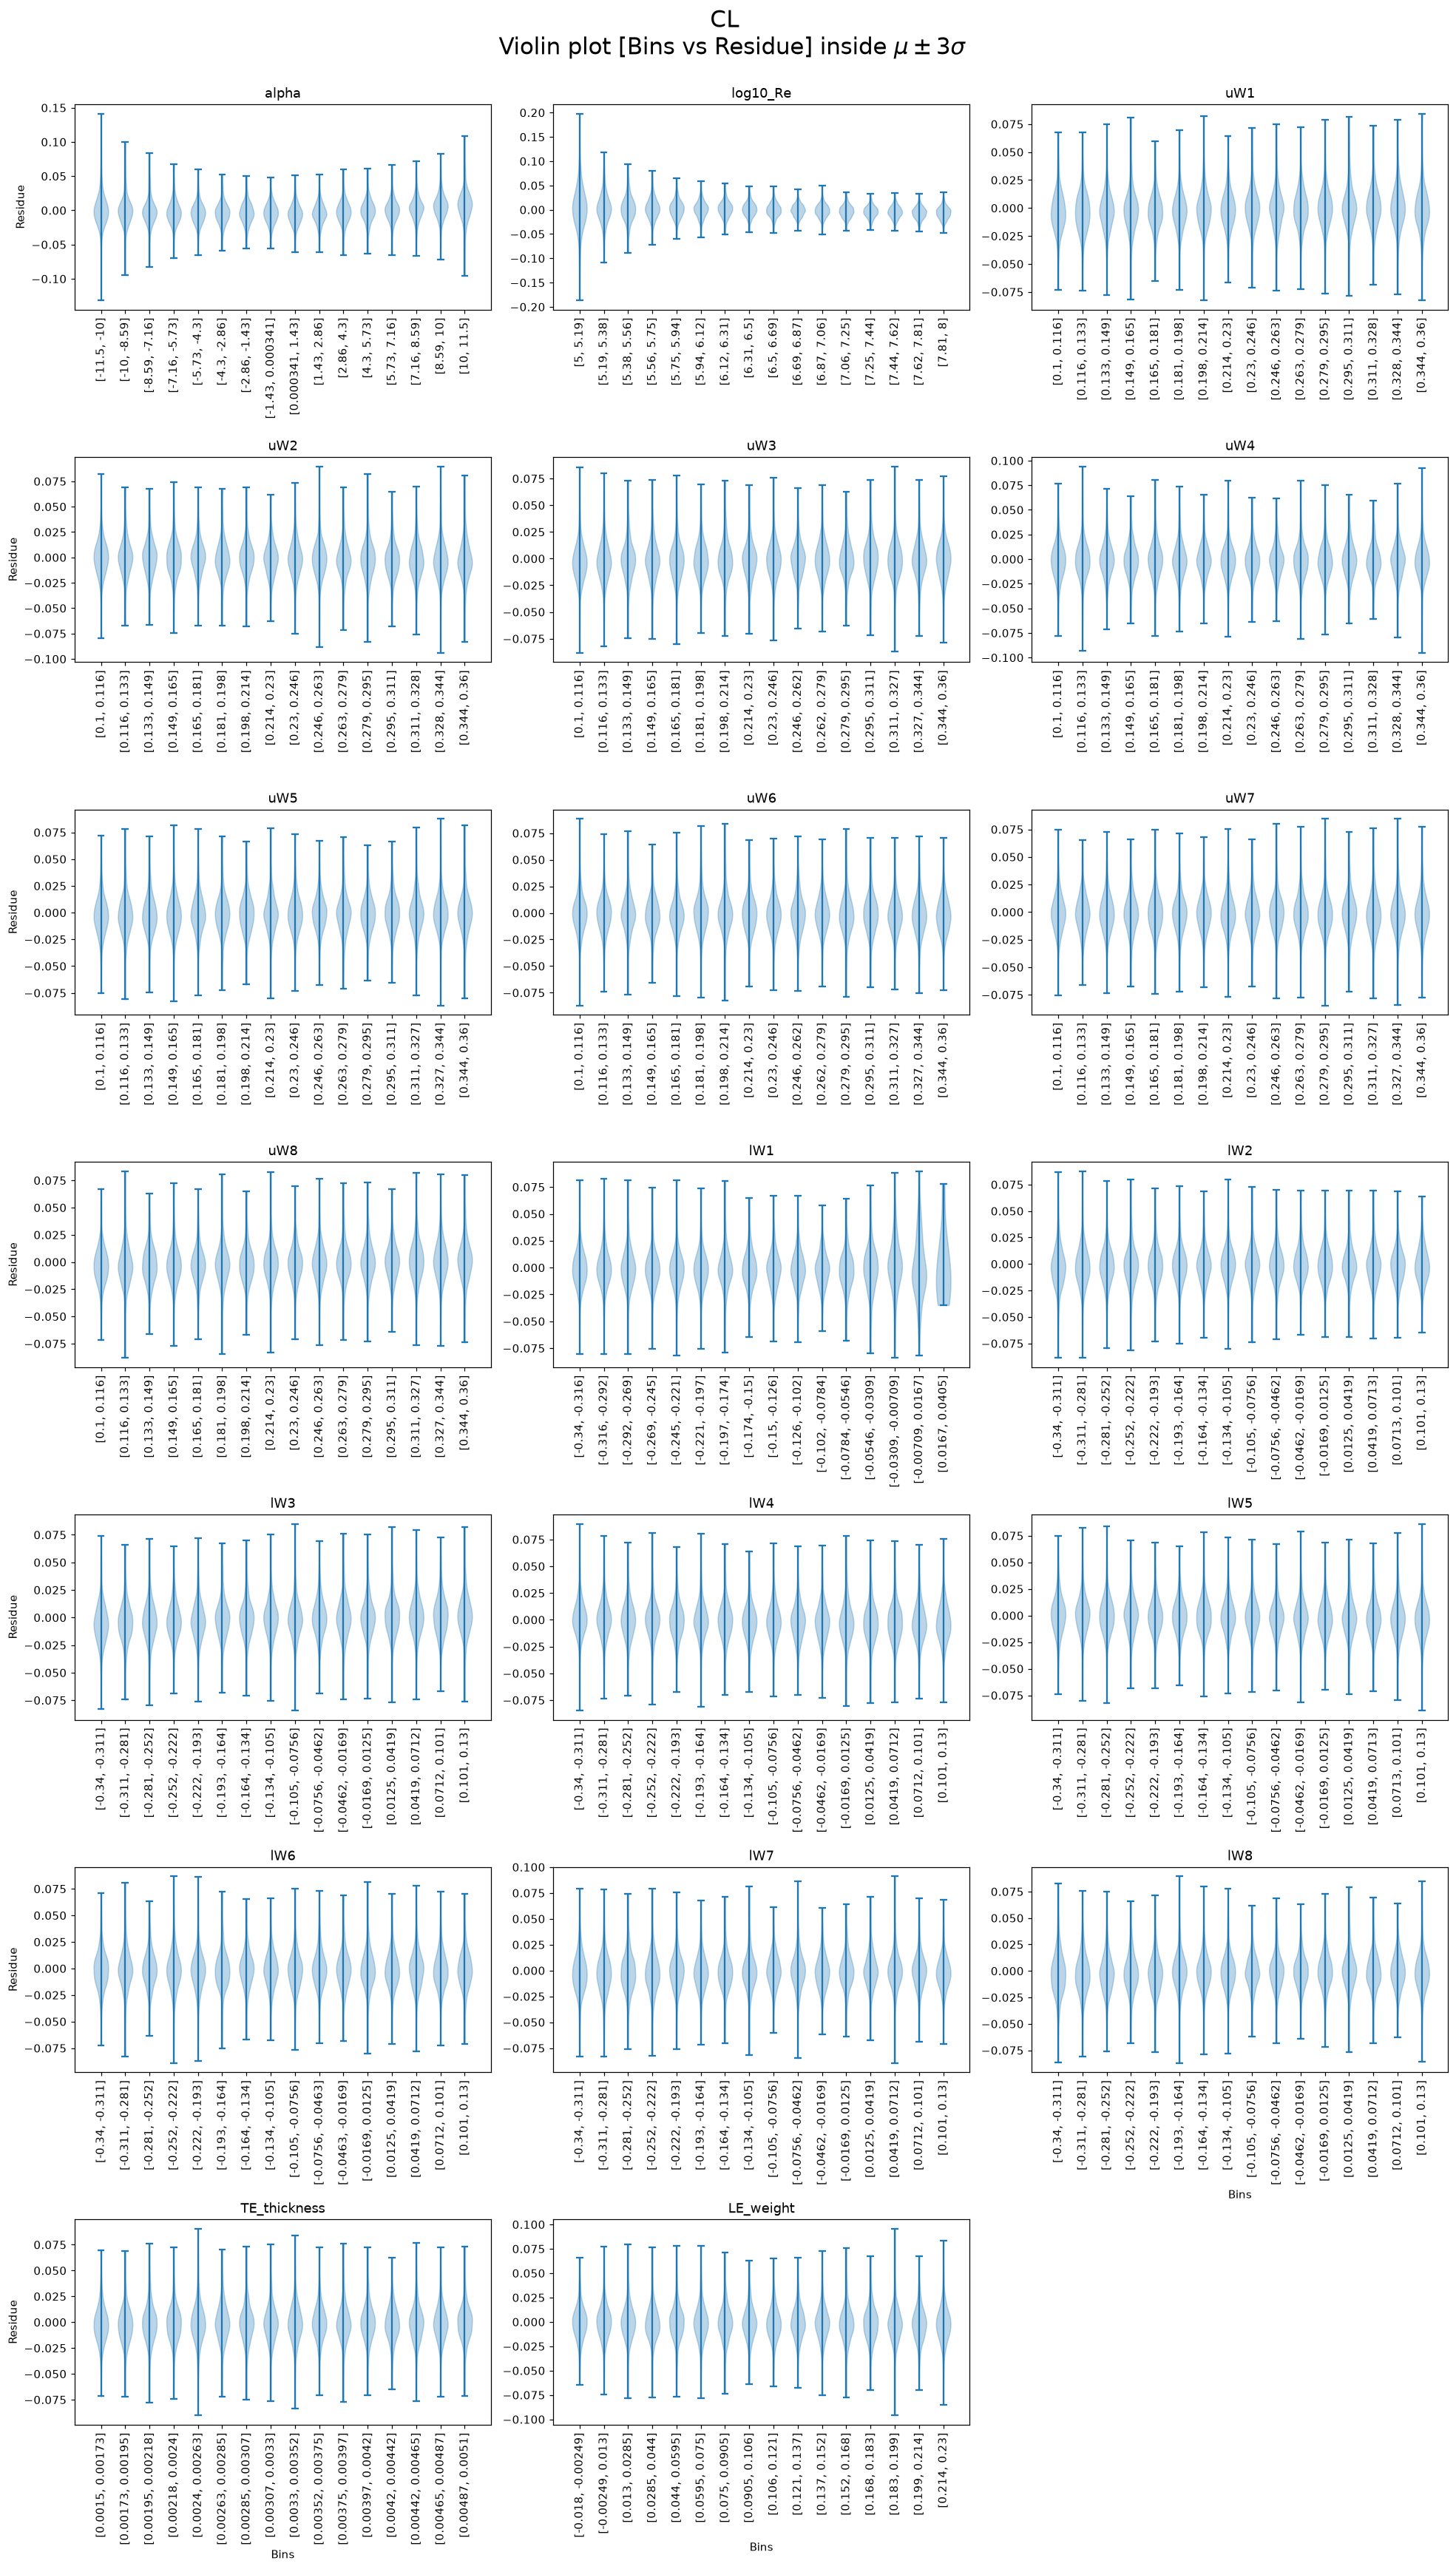
\includegraphics[width=1.0\linewidth,height=0.80\textheight,keepaspectratio]{analysis_plots/pex_violin_res_CL.png}\end{center}
\end{minipage}\par\medskip
\par\begin{minipage}{\linewidth}
\subsection*{\normalsize Residue --- CD}
\begin{center}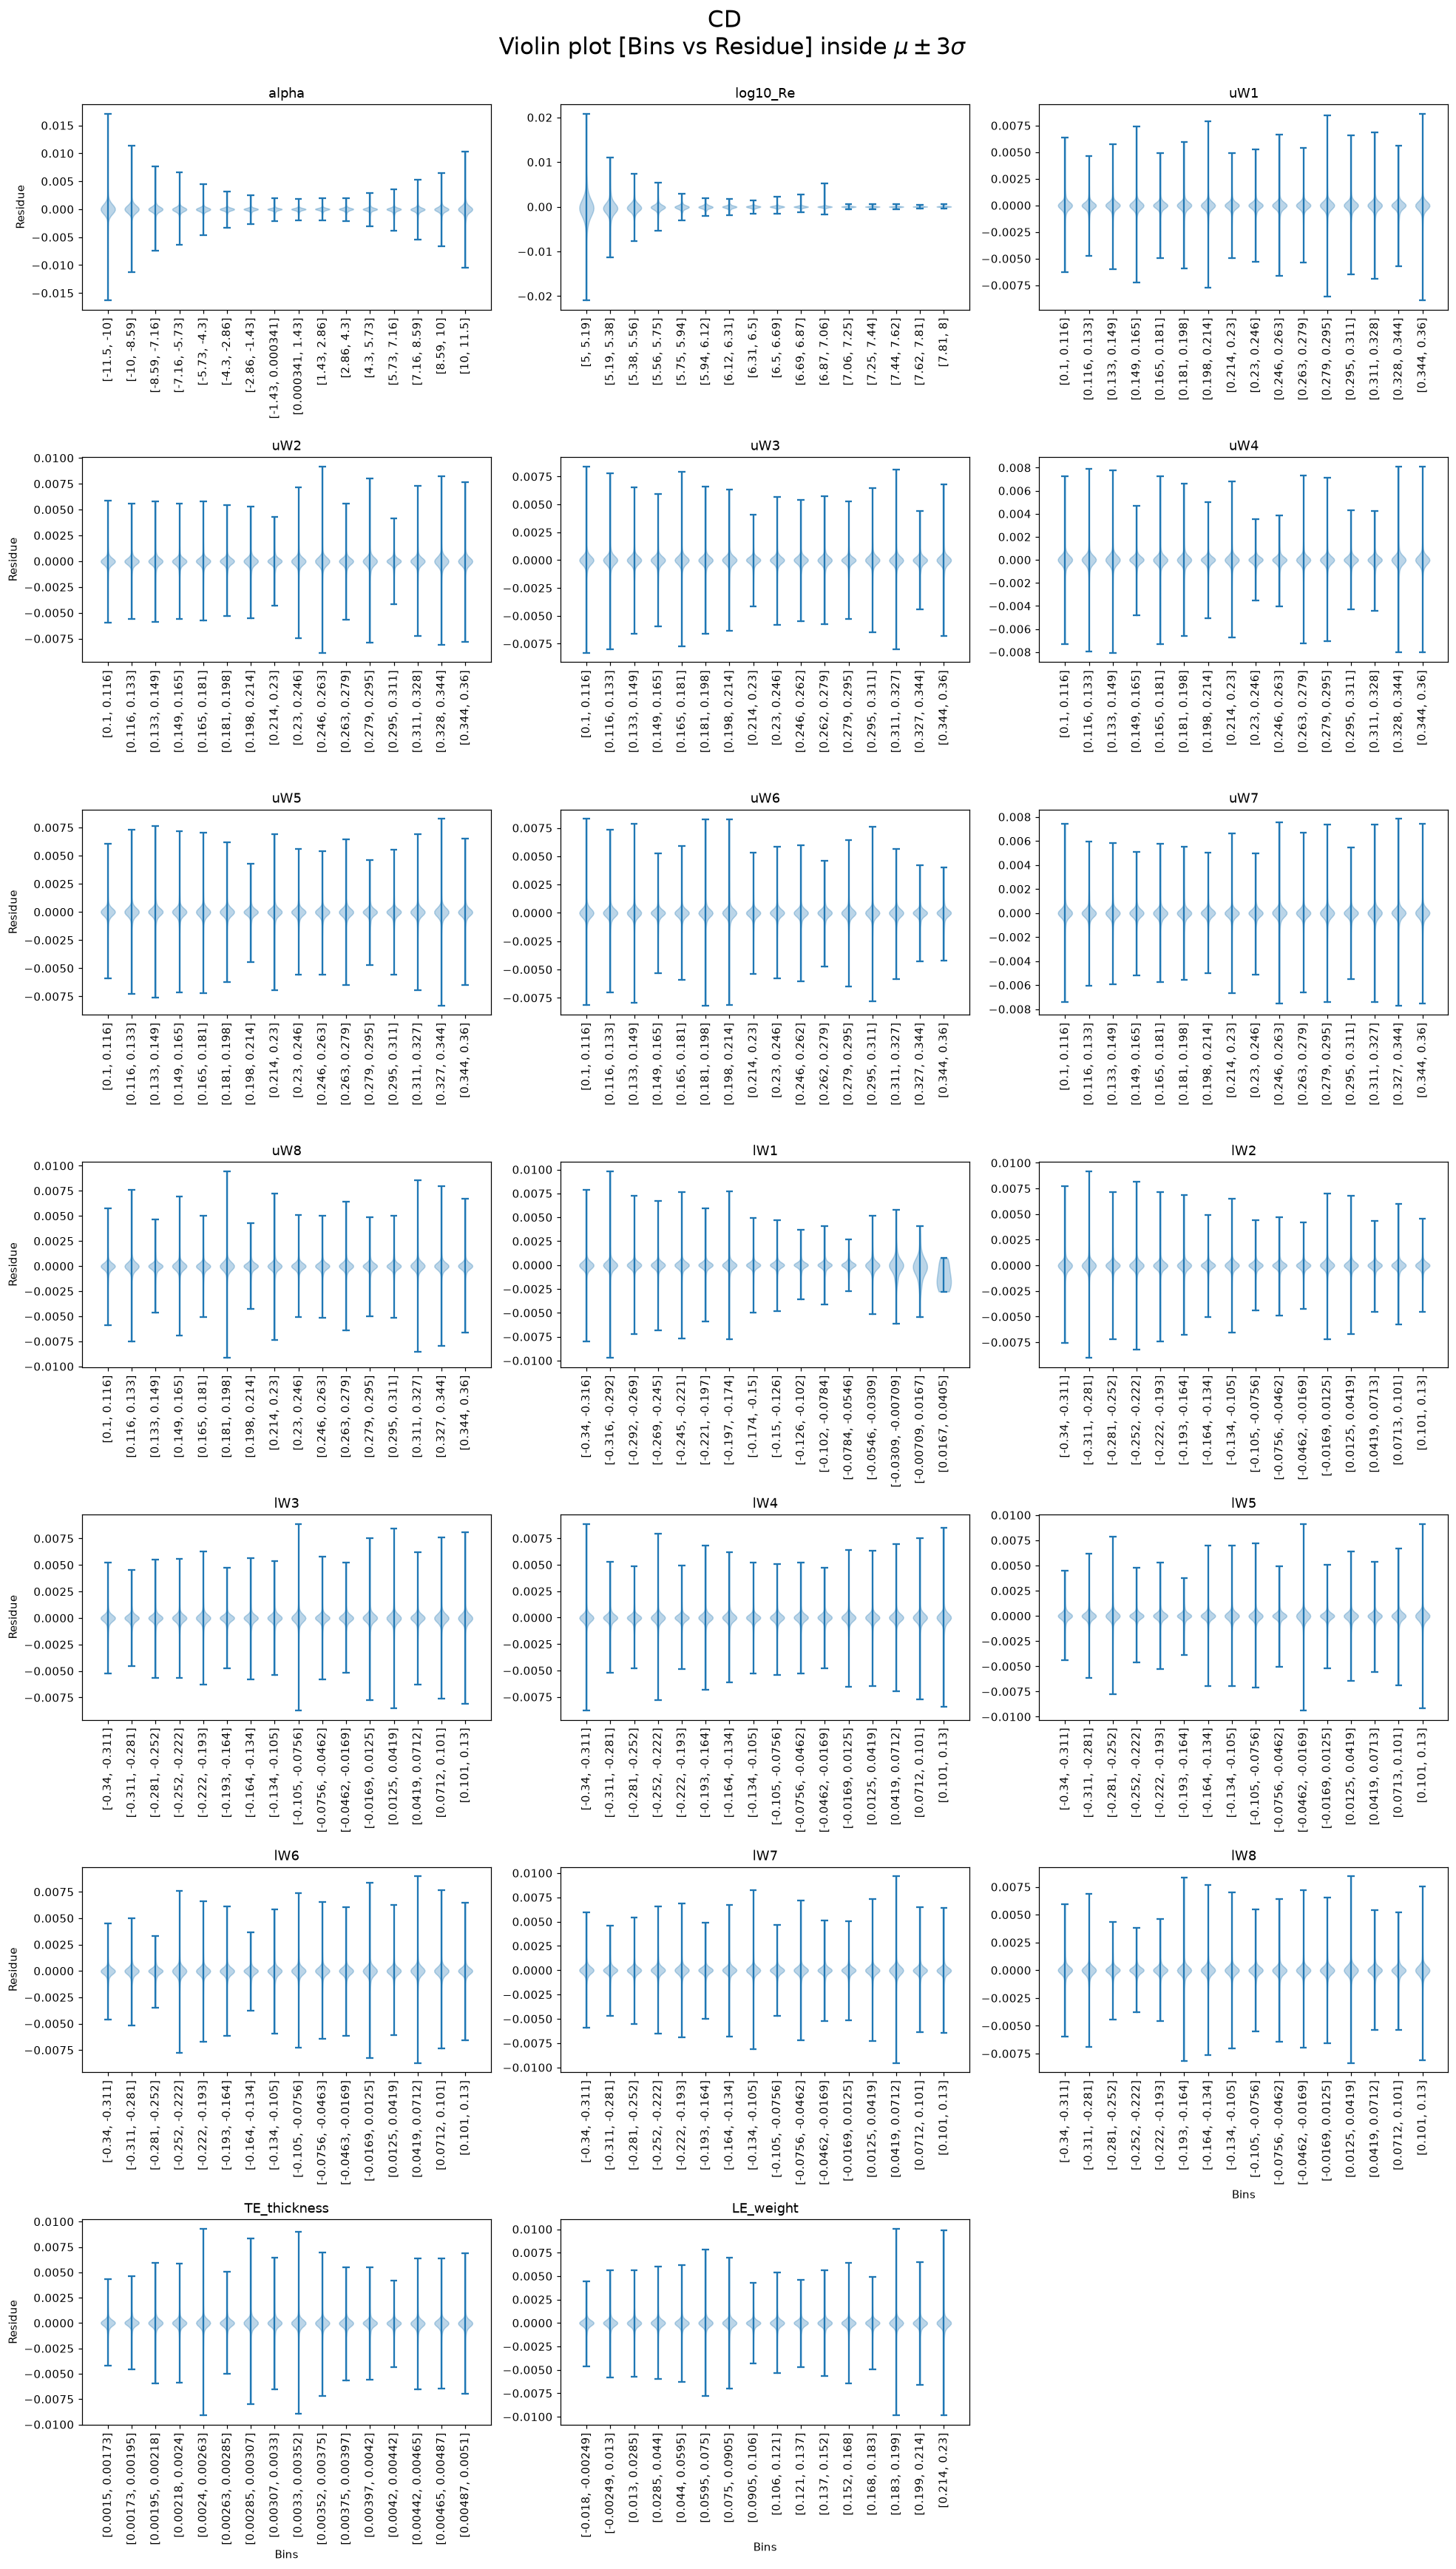
\includegraphics[width=1.0\linewidth,height=0.80\textheight,keepaspectratio]{analysis_plots/pex_violin_res_CD.png}\end{center}
\end{minipage}\par\medskip
\par\begin{minipage}{\linewidth}
\subsection*{\normalsize Residue --- CM}
\begin{center}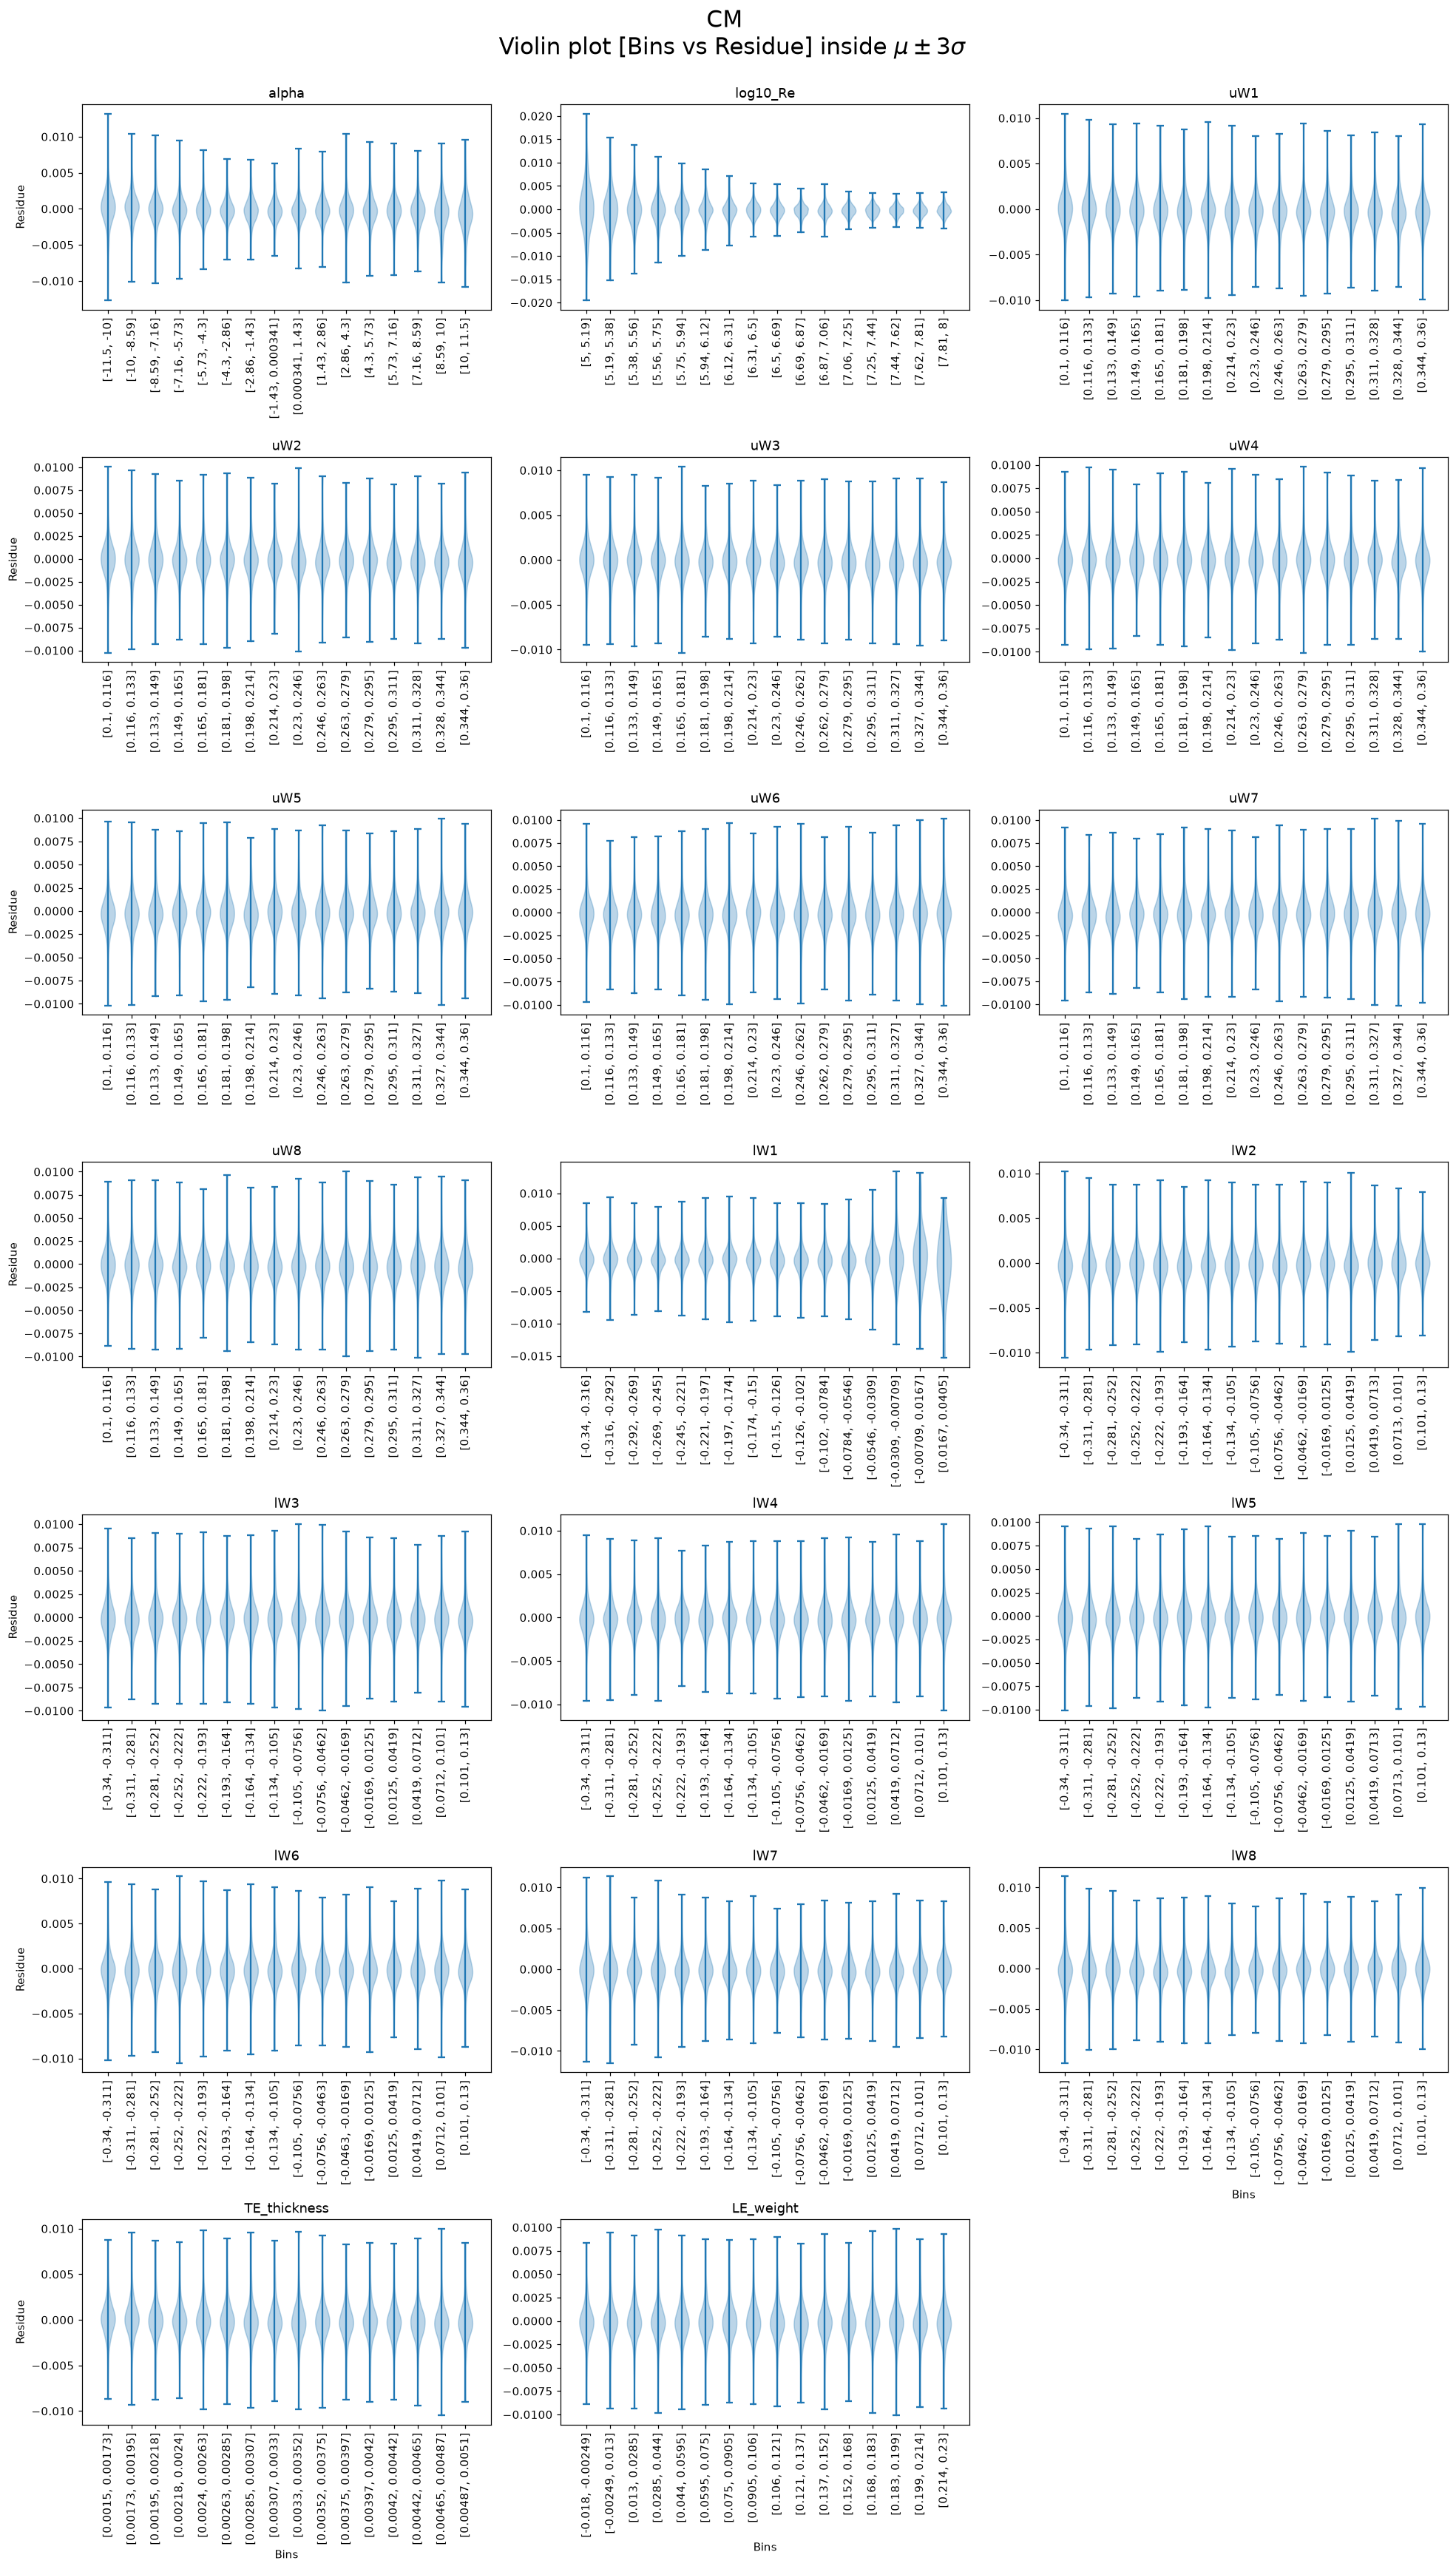
\includegraphics[width=1.0\linewidth,height=0.80\textheight,keepaspectratio]{analysis_plots/pex_violin_res_CM.png}\end{center}
\end{minipage}\par\medskip
\par\begin{minipage}{\linewidth}
\subsection*{\normalsize Residue --- top\_transition\_location}
\begin{center}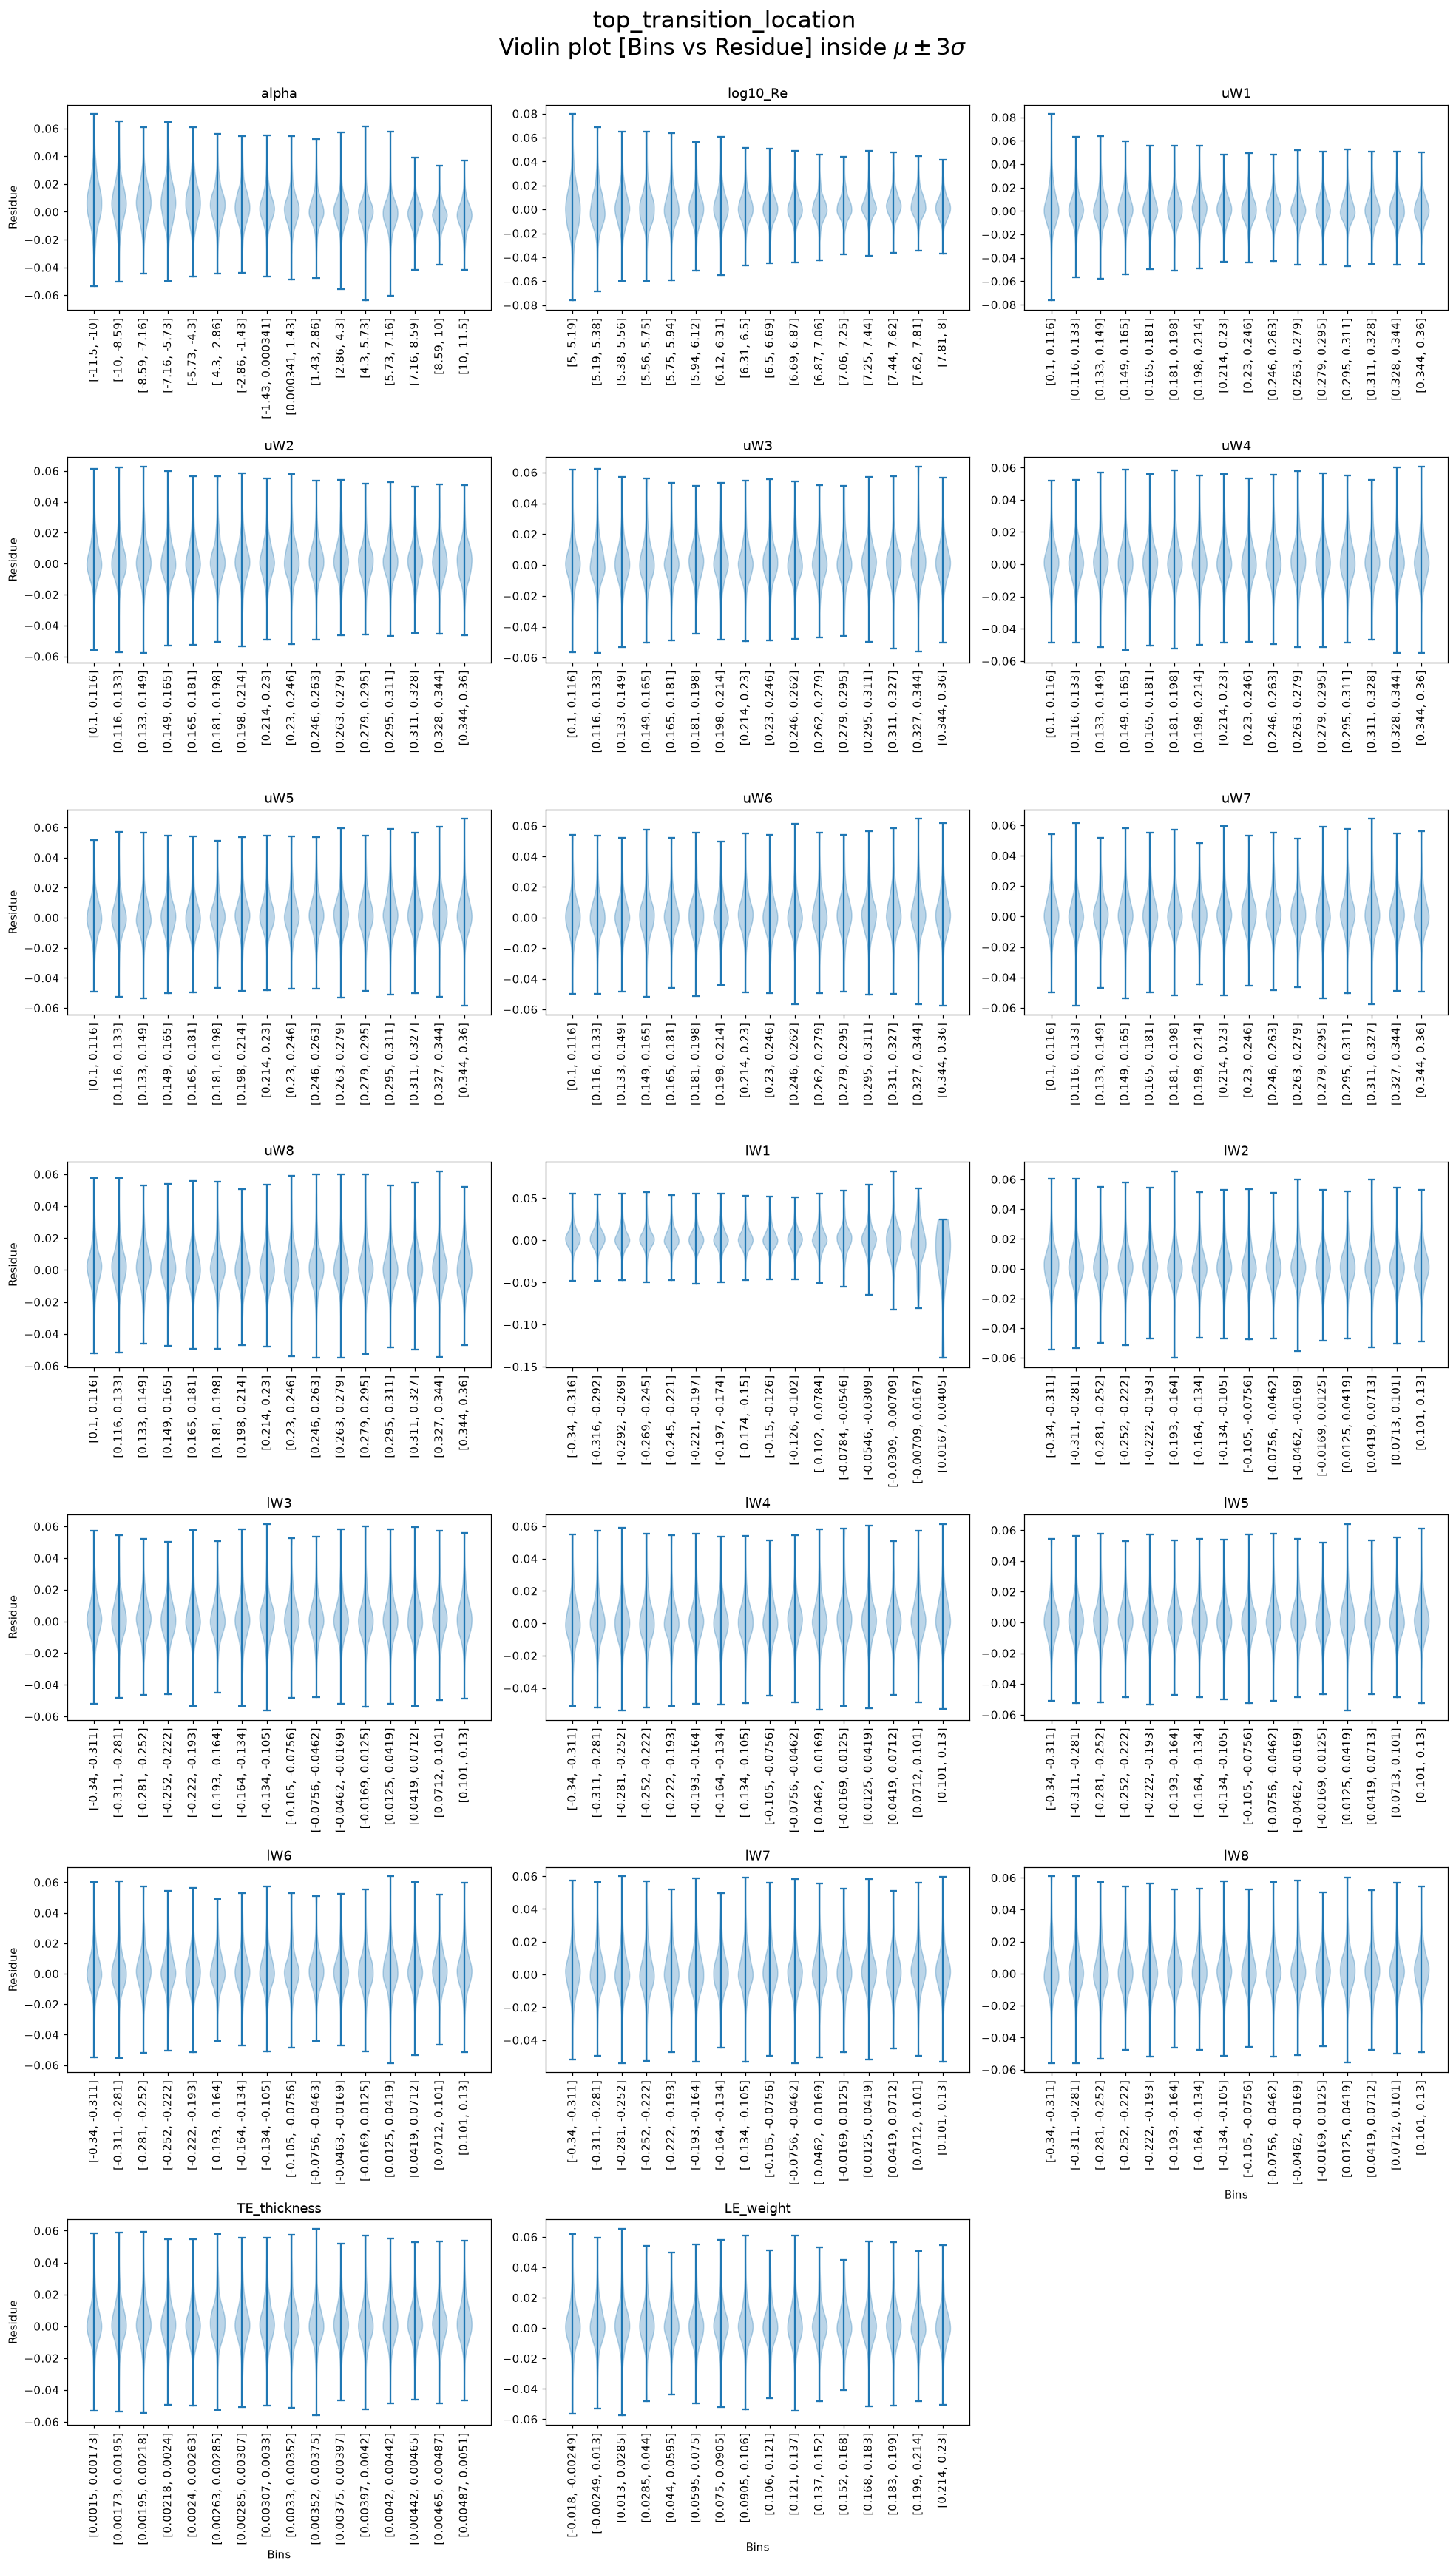
\includegraphics[width=1.0\linewidth,height=0.80\textheight,keepaspectratio]{analysis_plots/pex_violin_res_top_transition_location.png}\end{center}
\end{minipage}\par\medskip
\par\begin{minipage}{\linewidth}
\subsection*{\normalsize Residue --- bottom\_transition\_location}
\begin{center}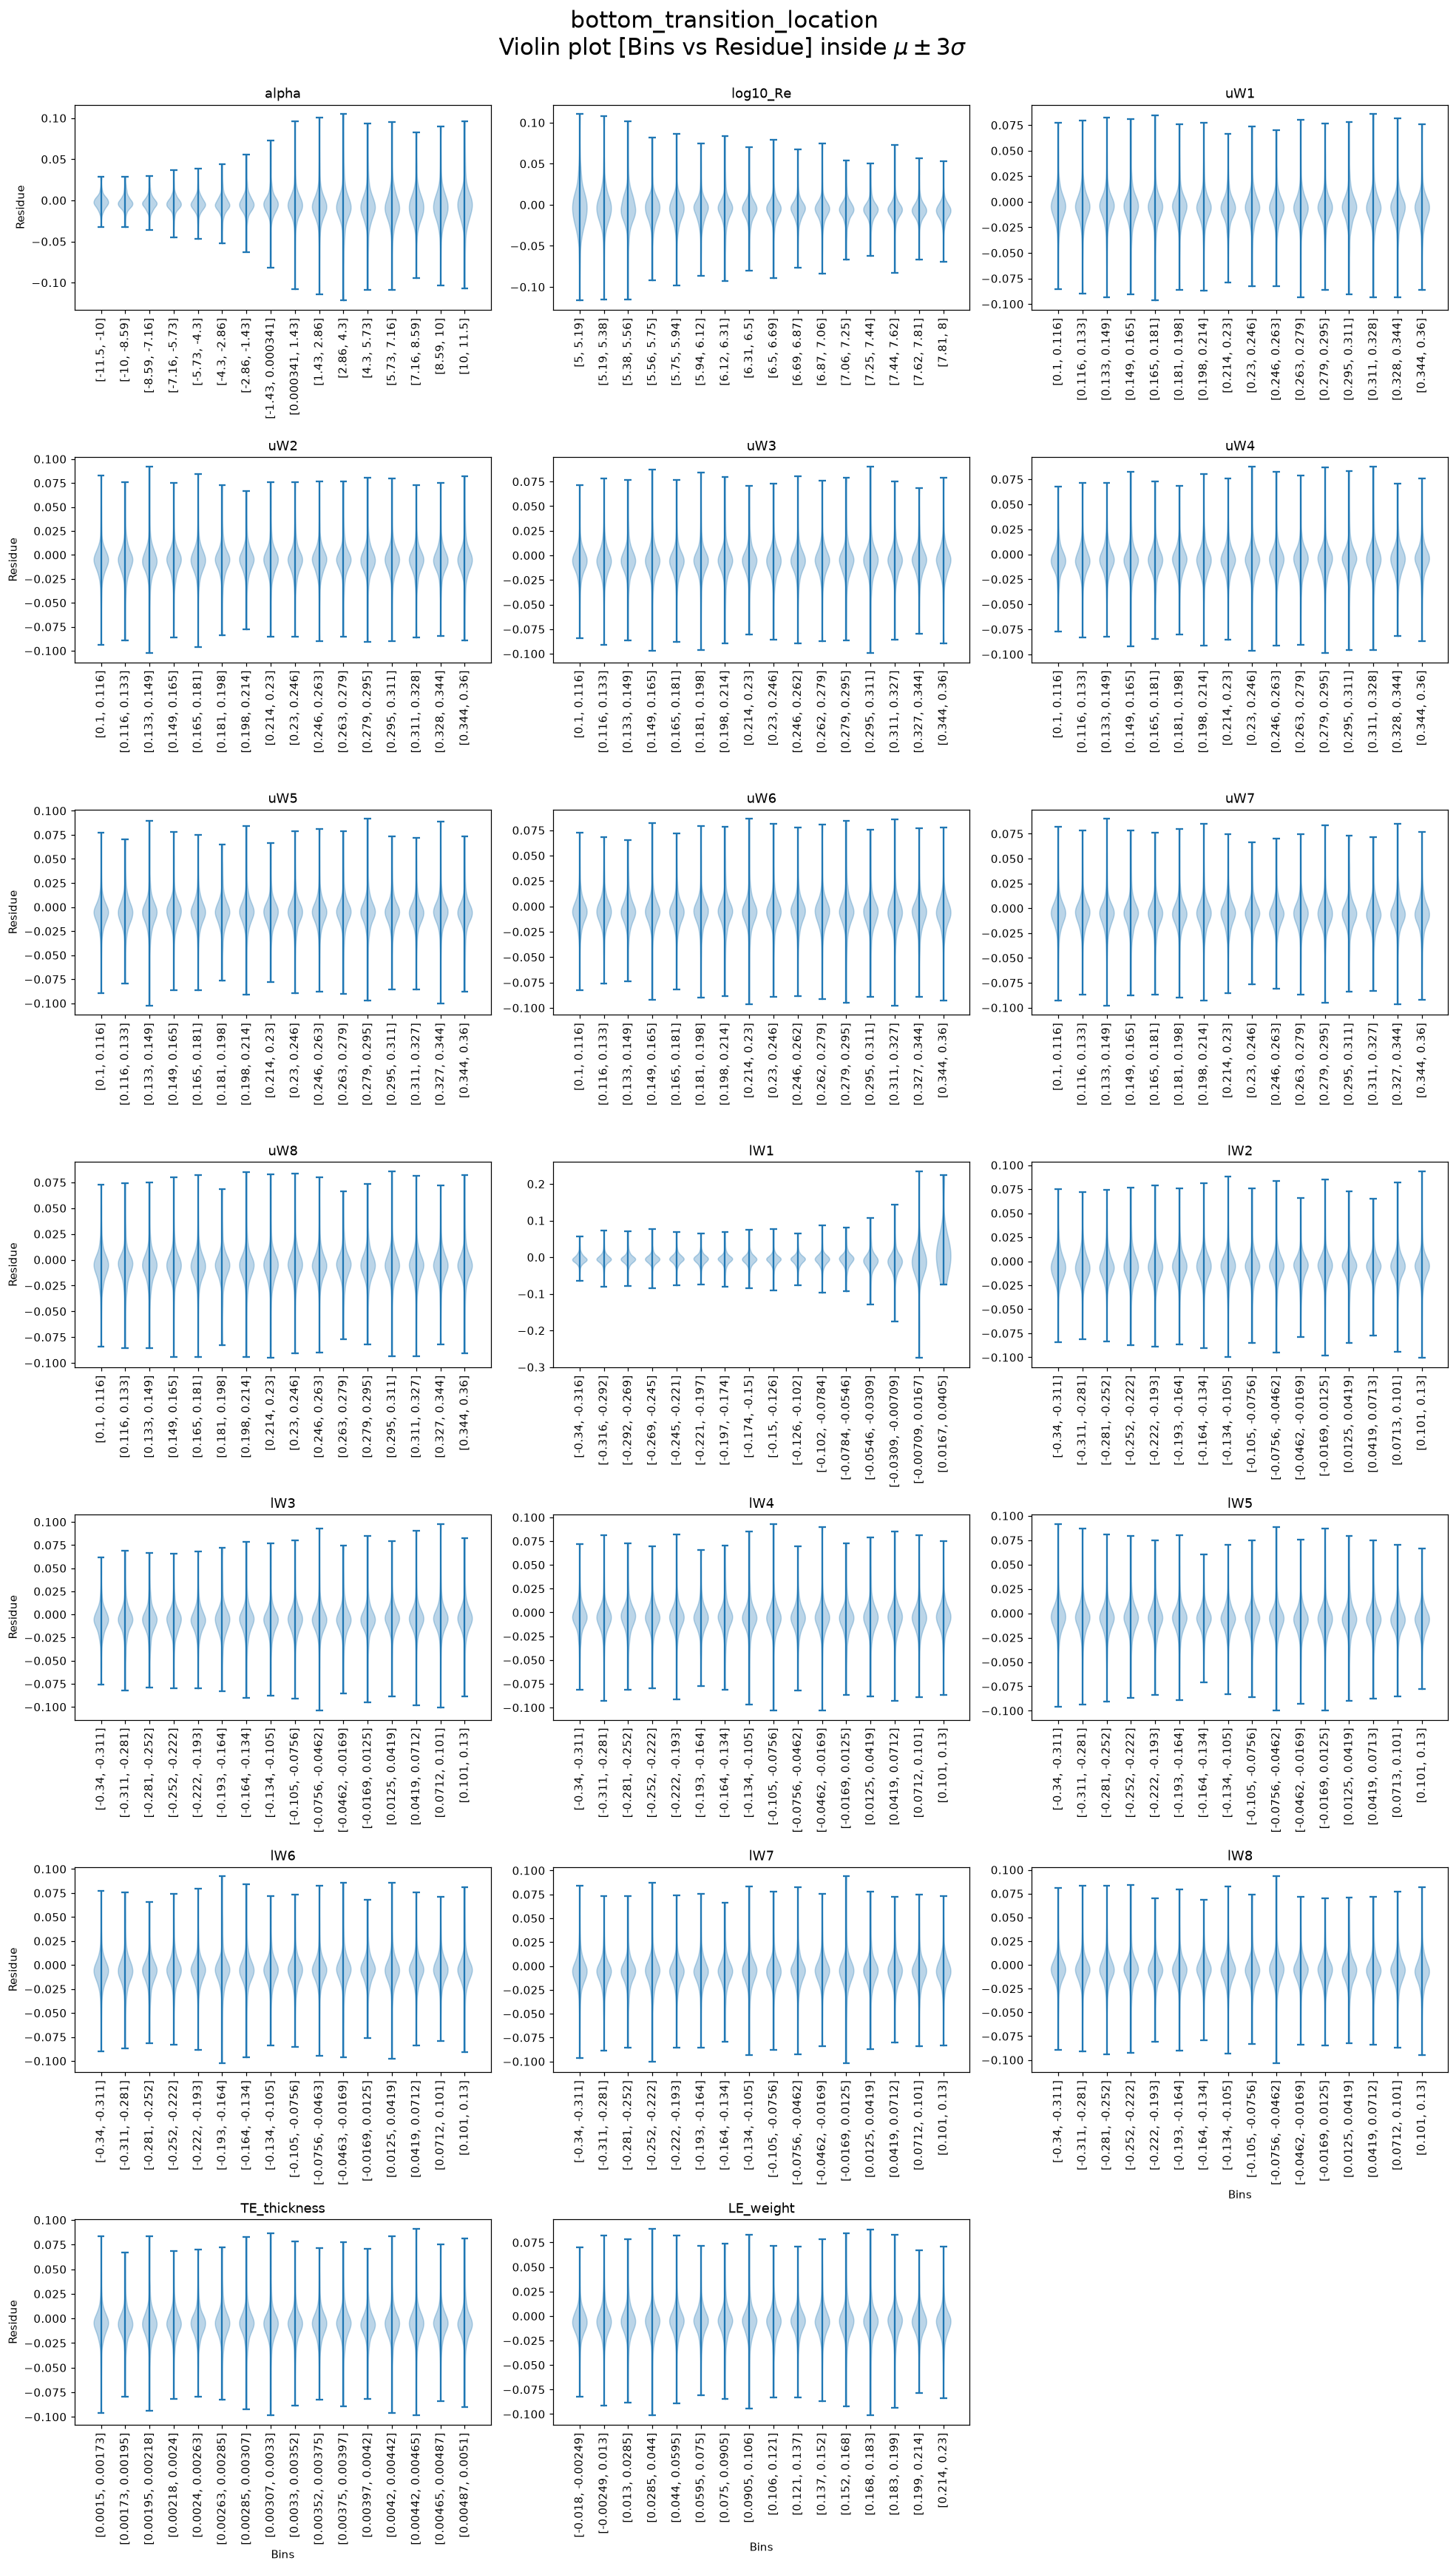
\includegraphics[width=1.0\linewidth,height=0.80\textheight,keepaspectratio]{analysis_plots/pex_violin_res_bottom_transition_location.png}\end{center}
\end{minipage}\par\medskip
\clearpage
\exhead{Absolute Error Violin Plots per Output (binned by input)}
\par\begin{minipage}{\linewidth}
\subsection*{\normalsize Absolute Error --- CL}
\begin{center}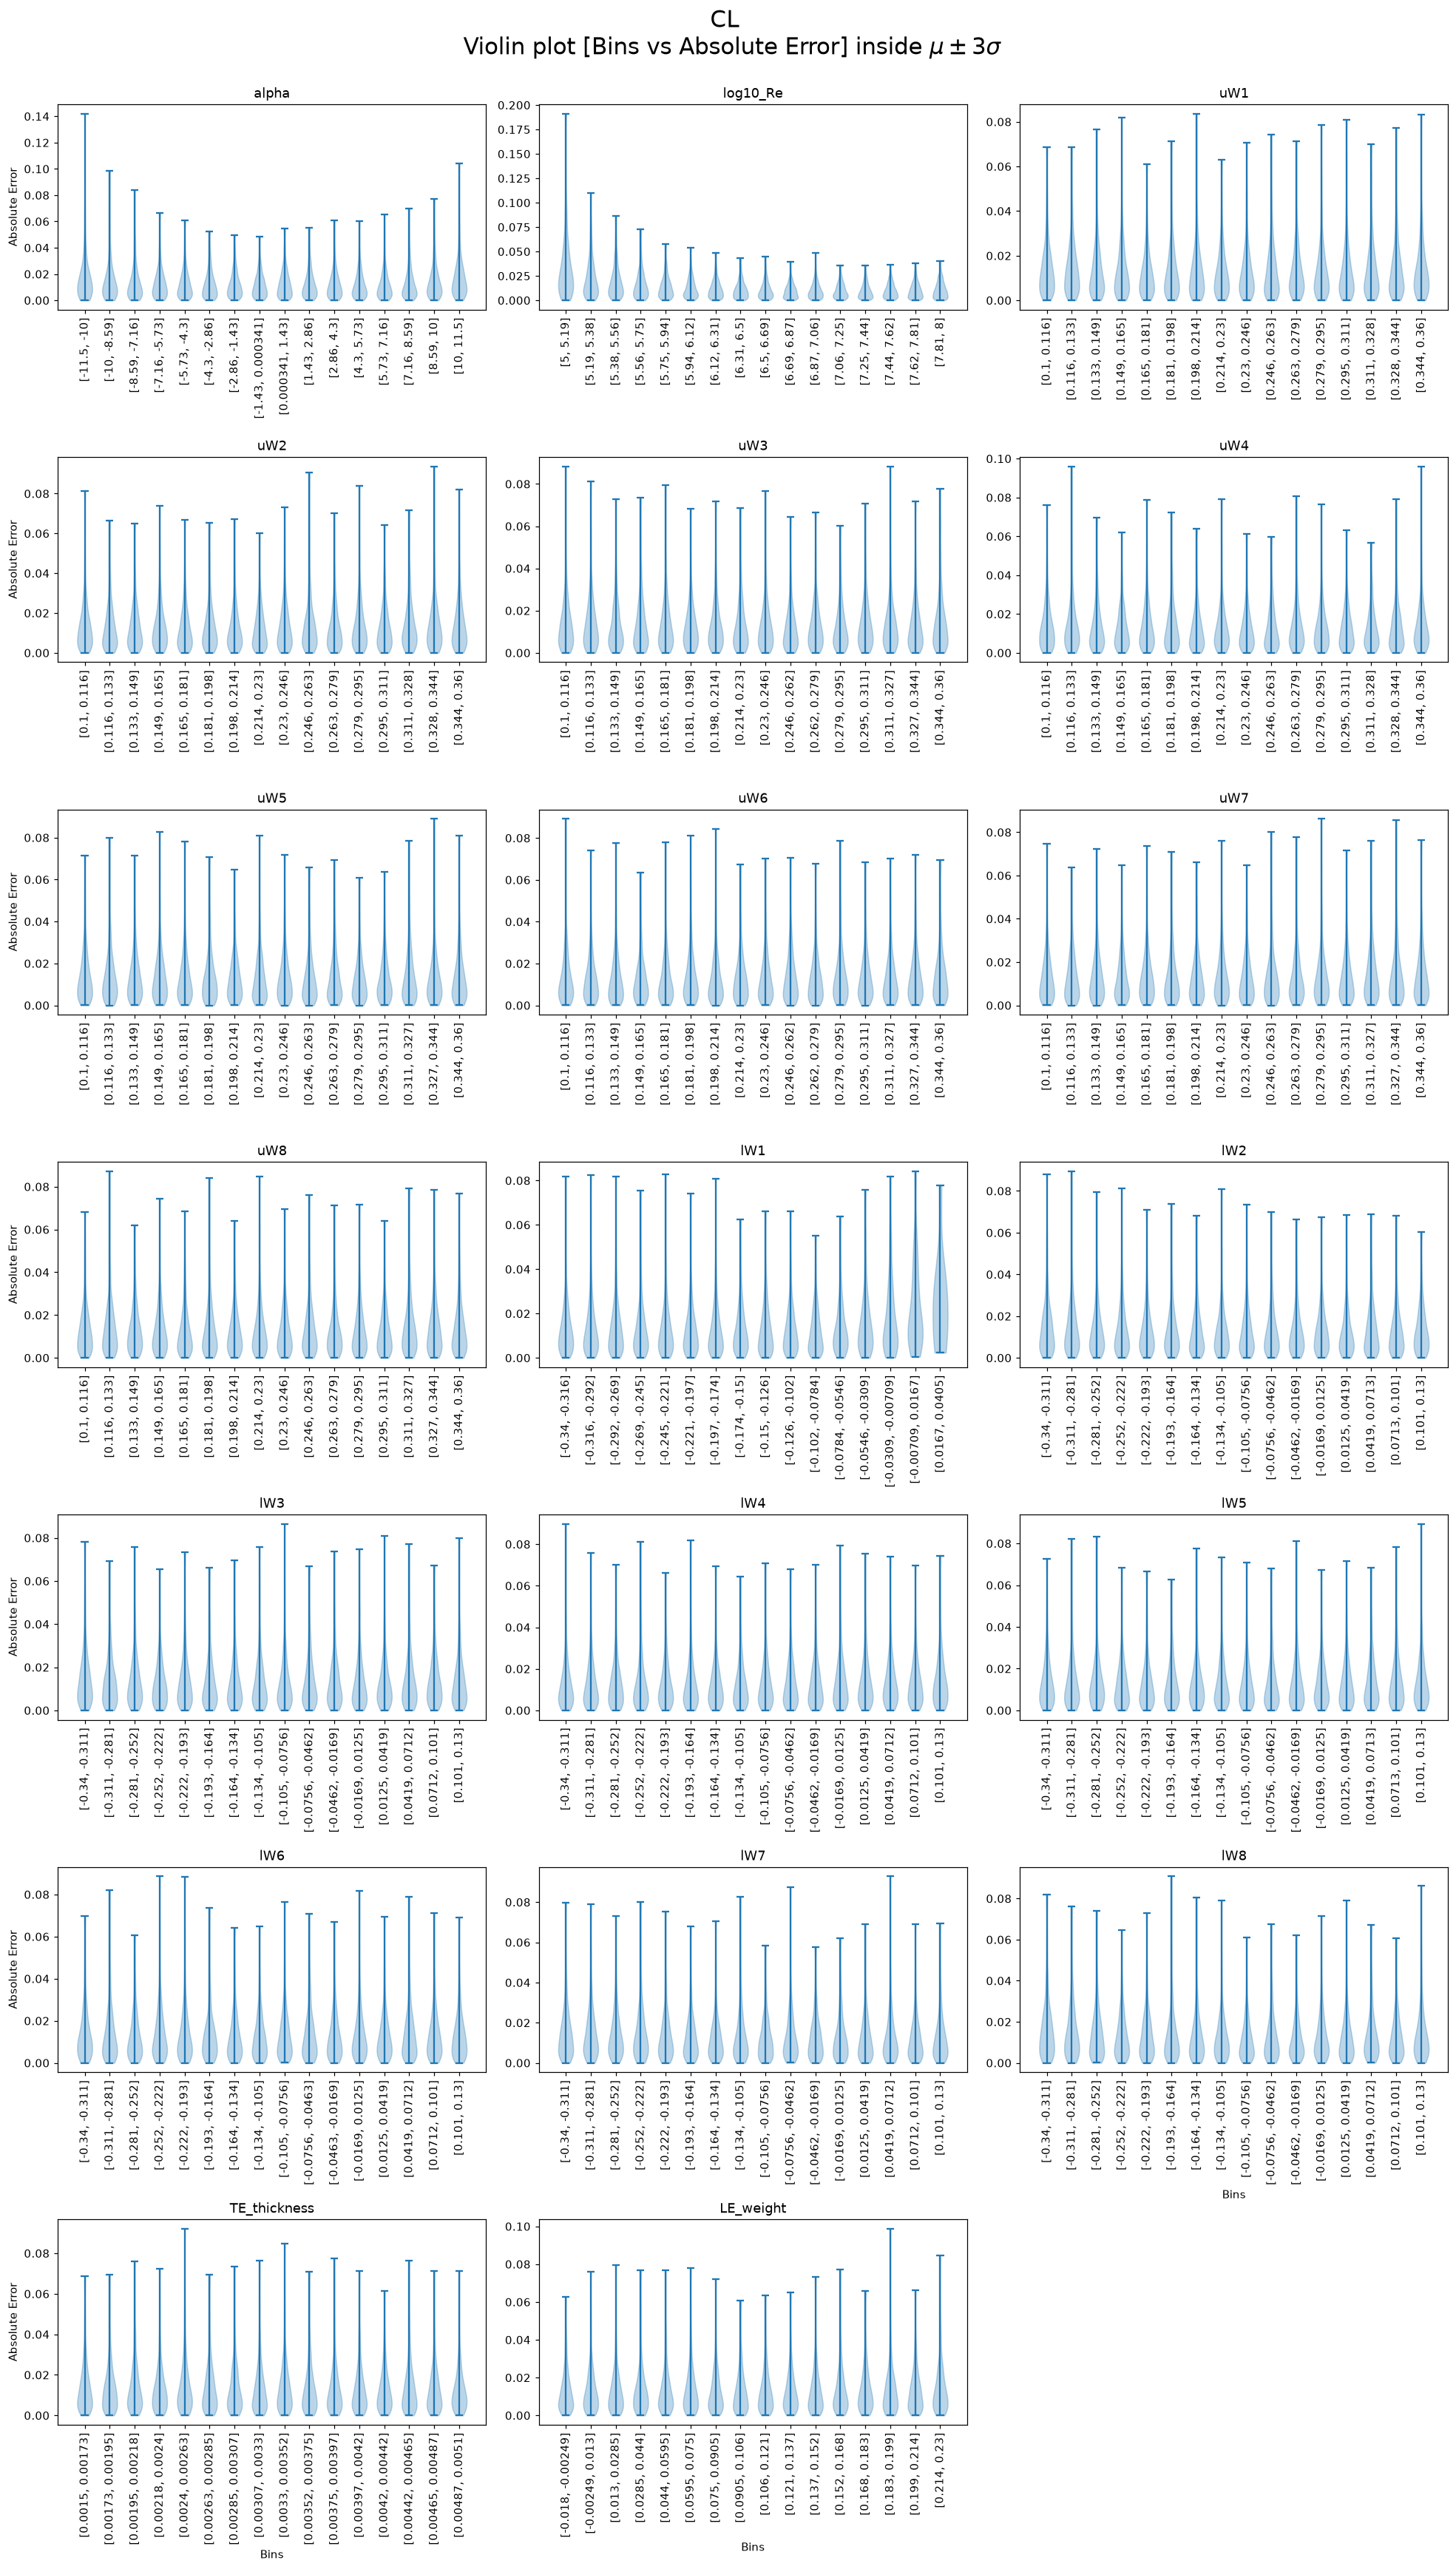
\includegraphics[width=1.0\linewidth,height=0.80\textheight,keepaspectratio]{analysis_plots/pex_violin_abs_CL.png}\end{center}
\end{minipage}\par\medskip
\par\begin{minipage}{\linewidth}
\subsection*{\normalsize Absolute Error --- CD}
\begin{center}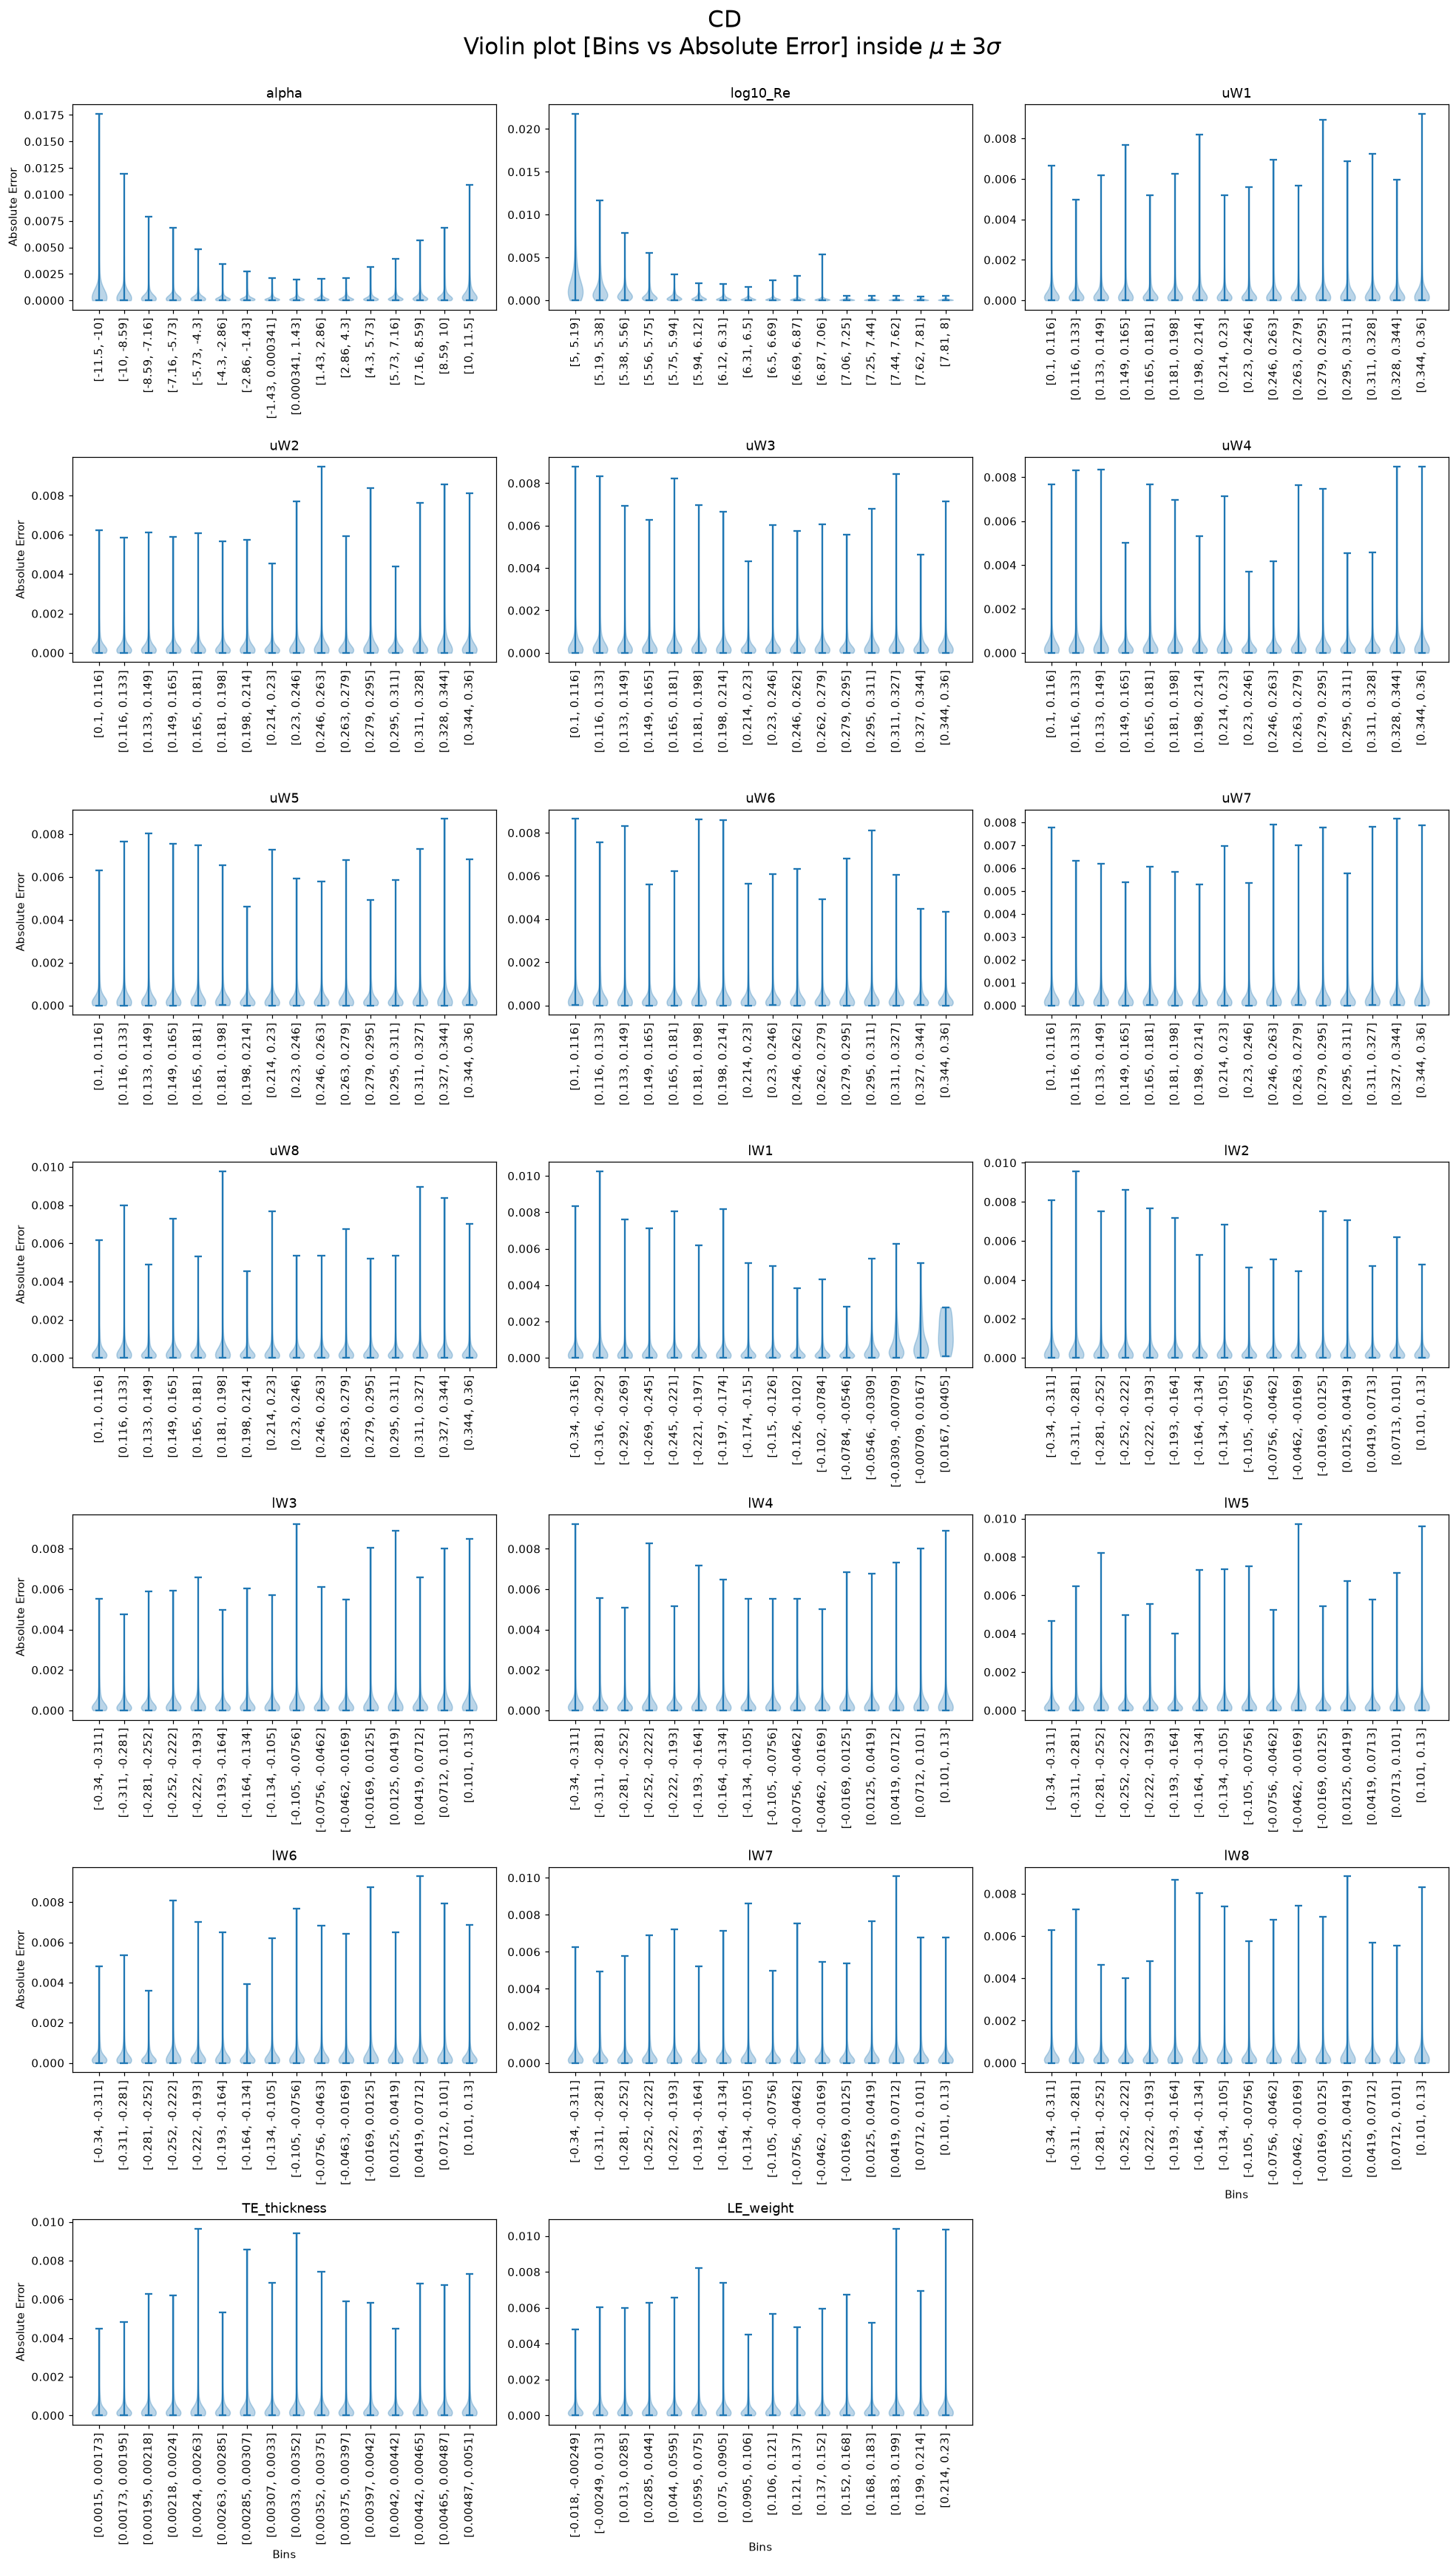
\includegraphics[width=1.0\linewidth,height=0.80\textheight,keepaspectratio]{analysis_plots/pex_violin_abs_CD.png}\end{center}
\end{minipage}\par\medskip
\par\begin{minipage}{\linewidth}
\subsection*{\normalsize Absolute Error --- CM}
\begin{center}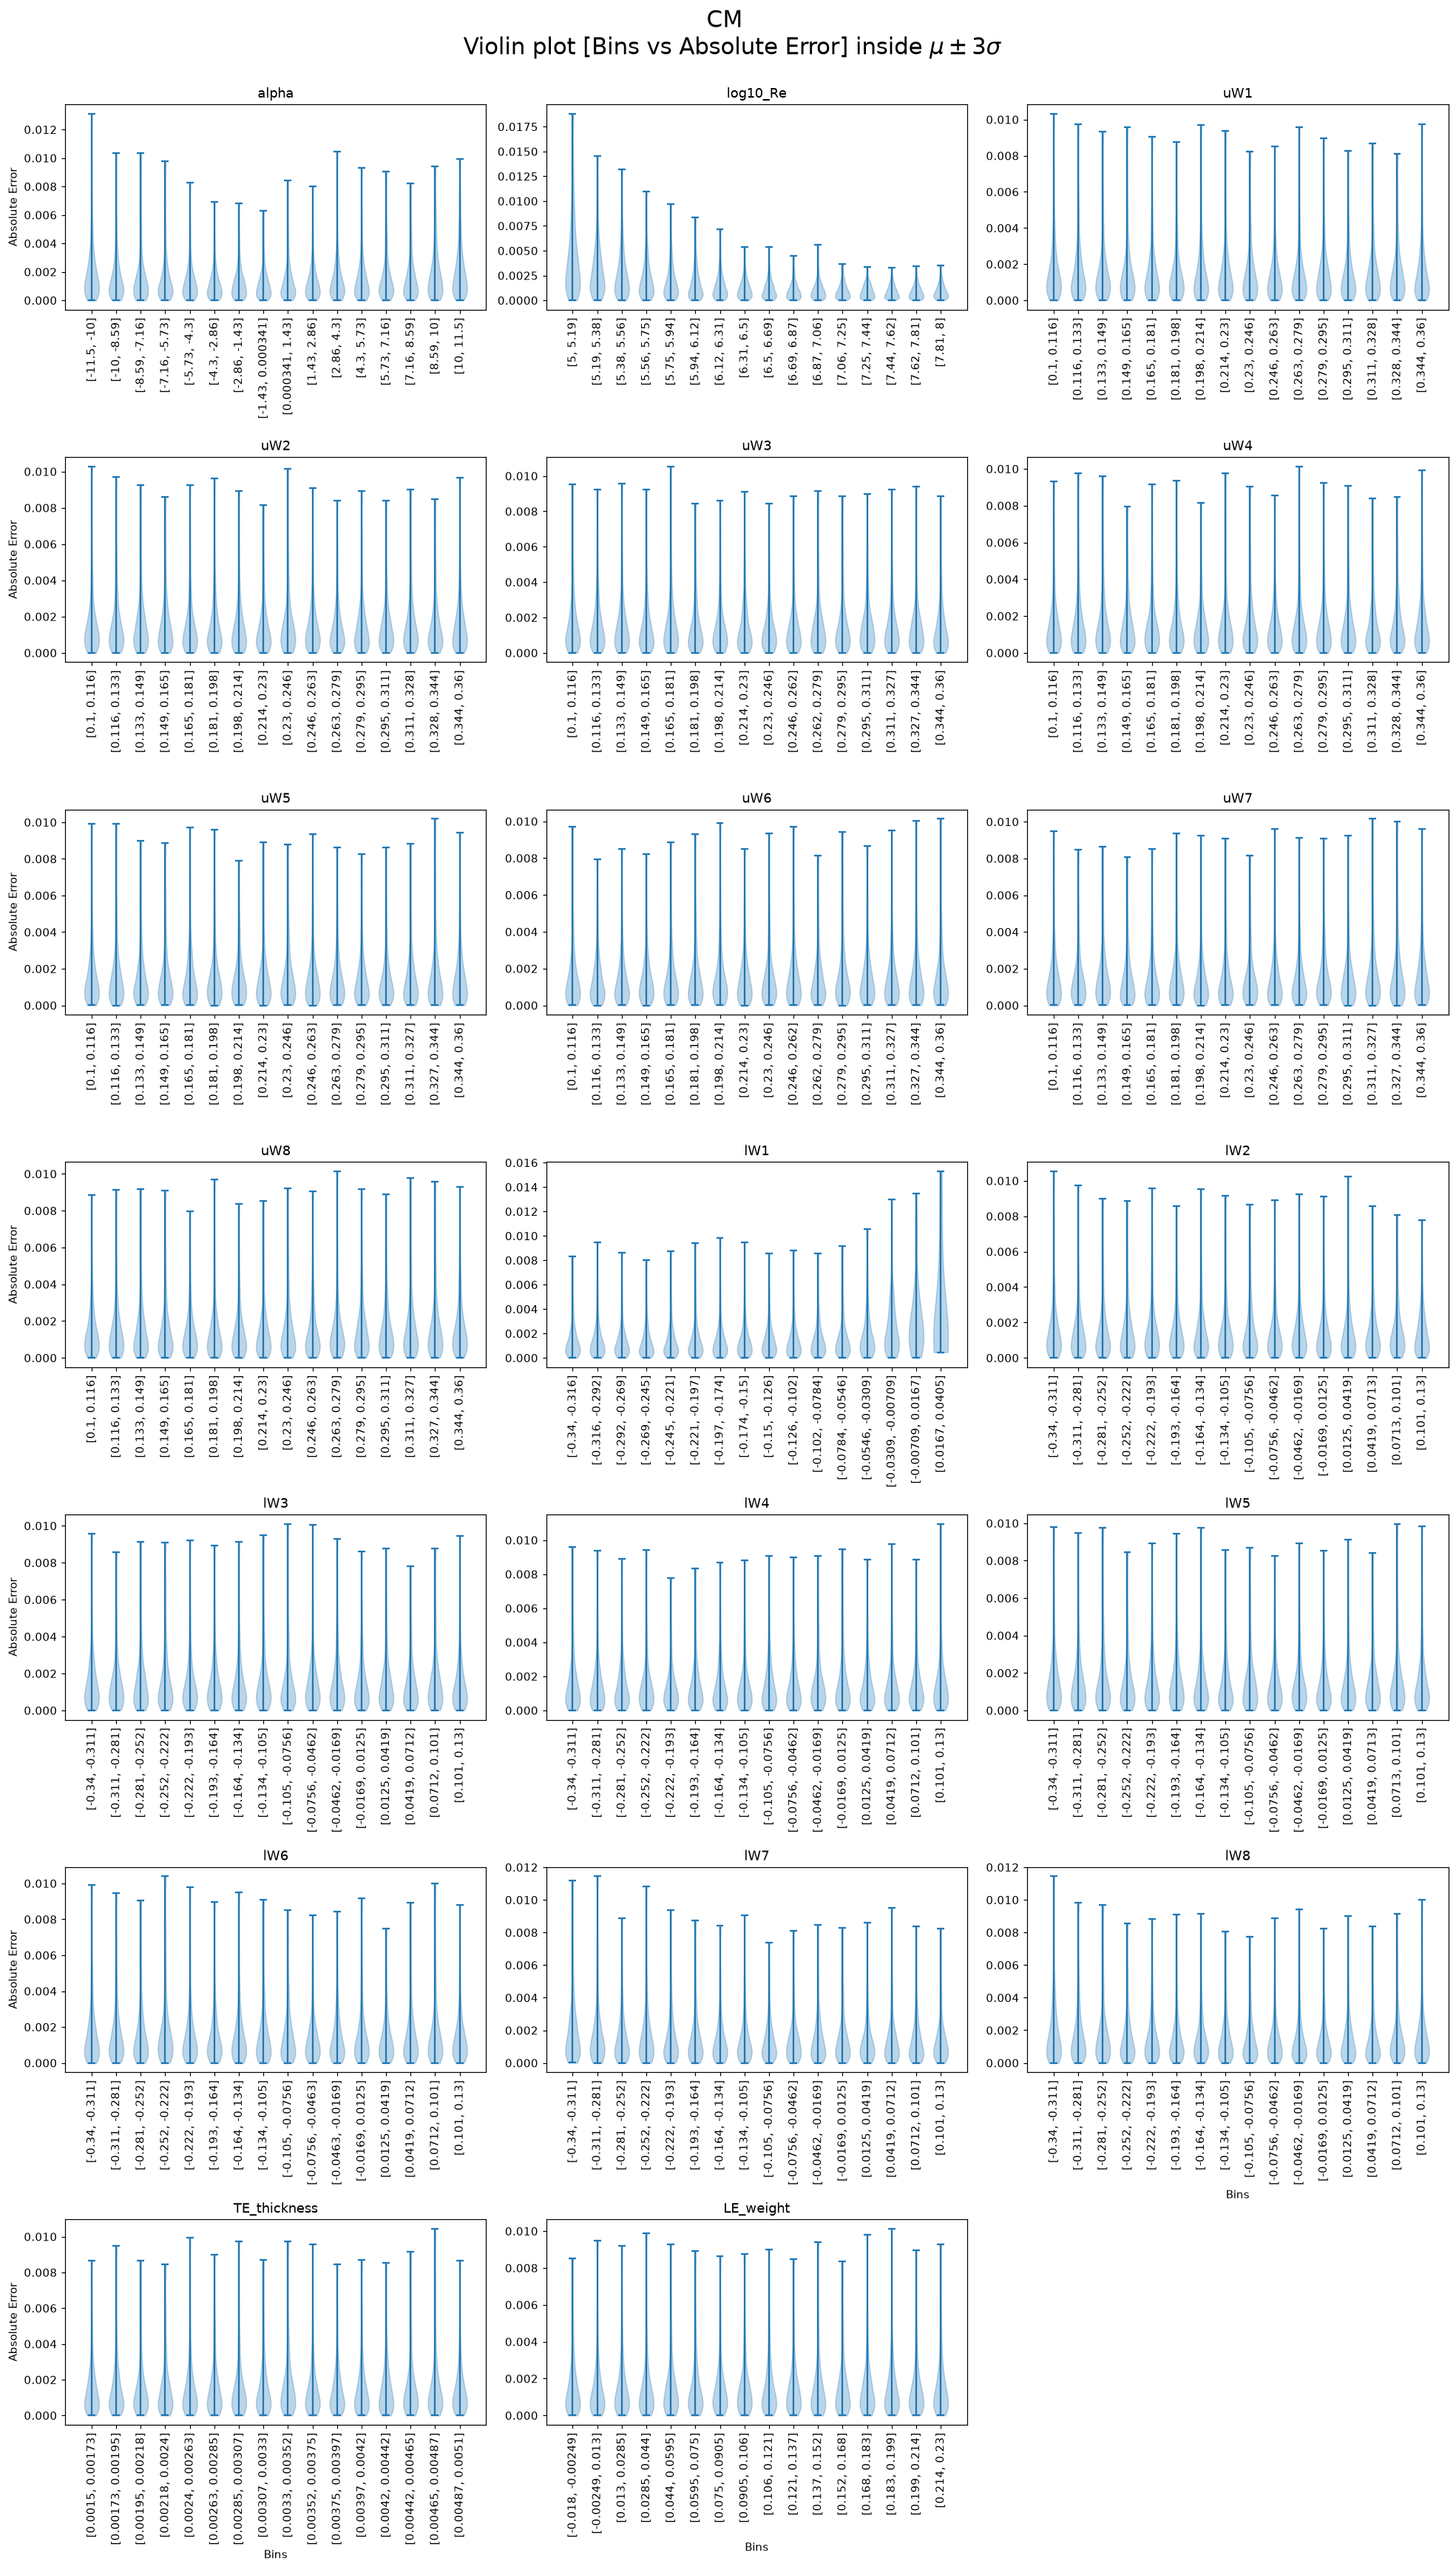
\includegraphics[width=1.0\linewidth,height=0.80\textheight,keepaspectratio]{analysis_plots/pex_violin_abs_CM.png}\end{center}
\end{minipage}\par\medskip
\par\begin{minipage}{\linewidth}
\subsection*{\normalsize Absolute Error --- top\_transition\_location}
\begin{center}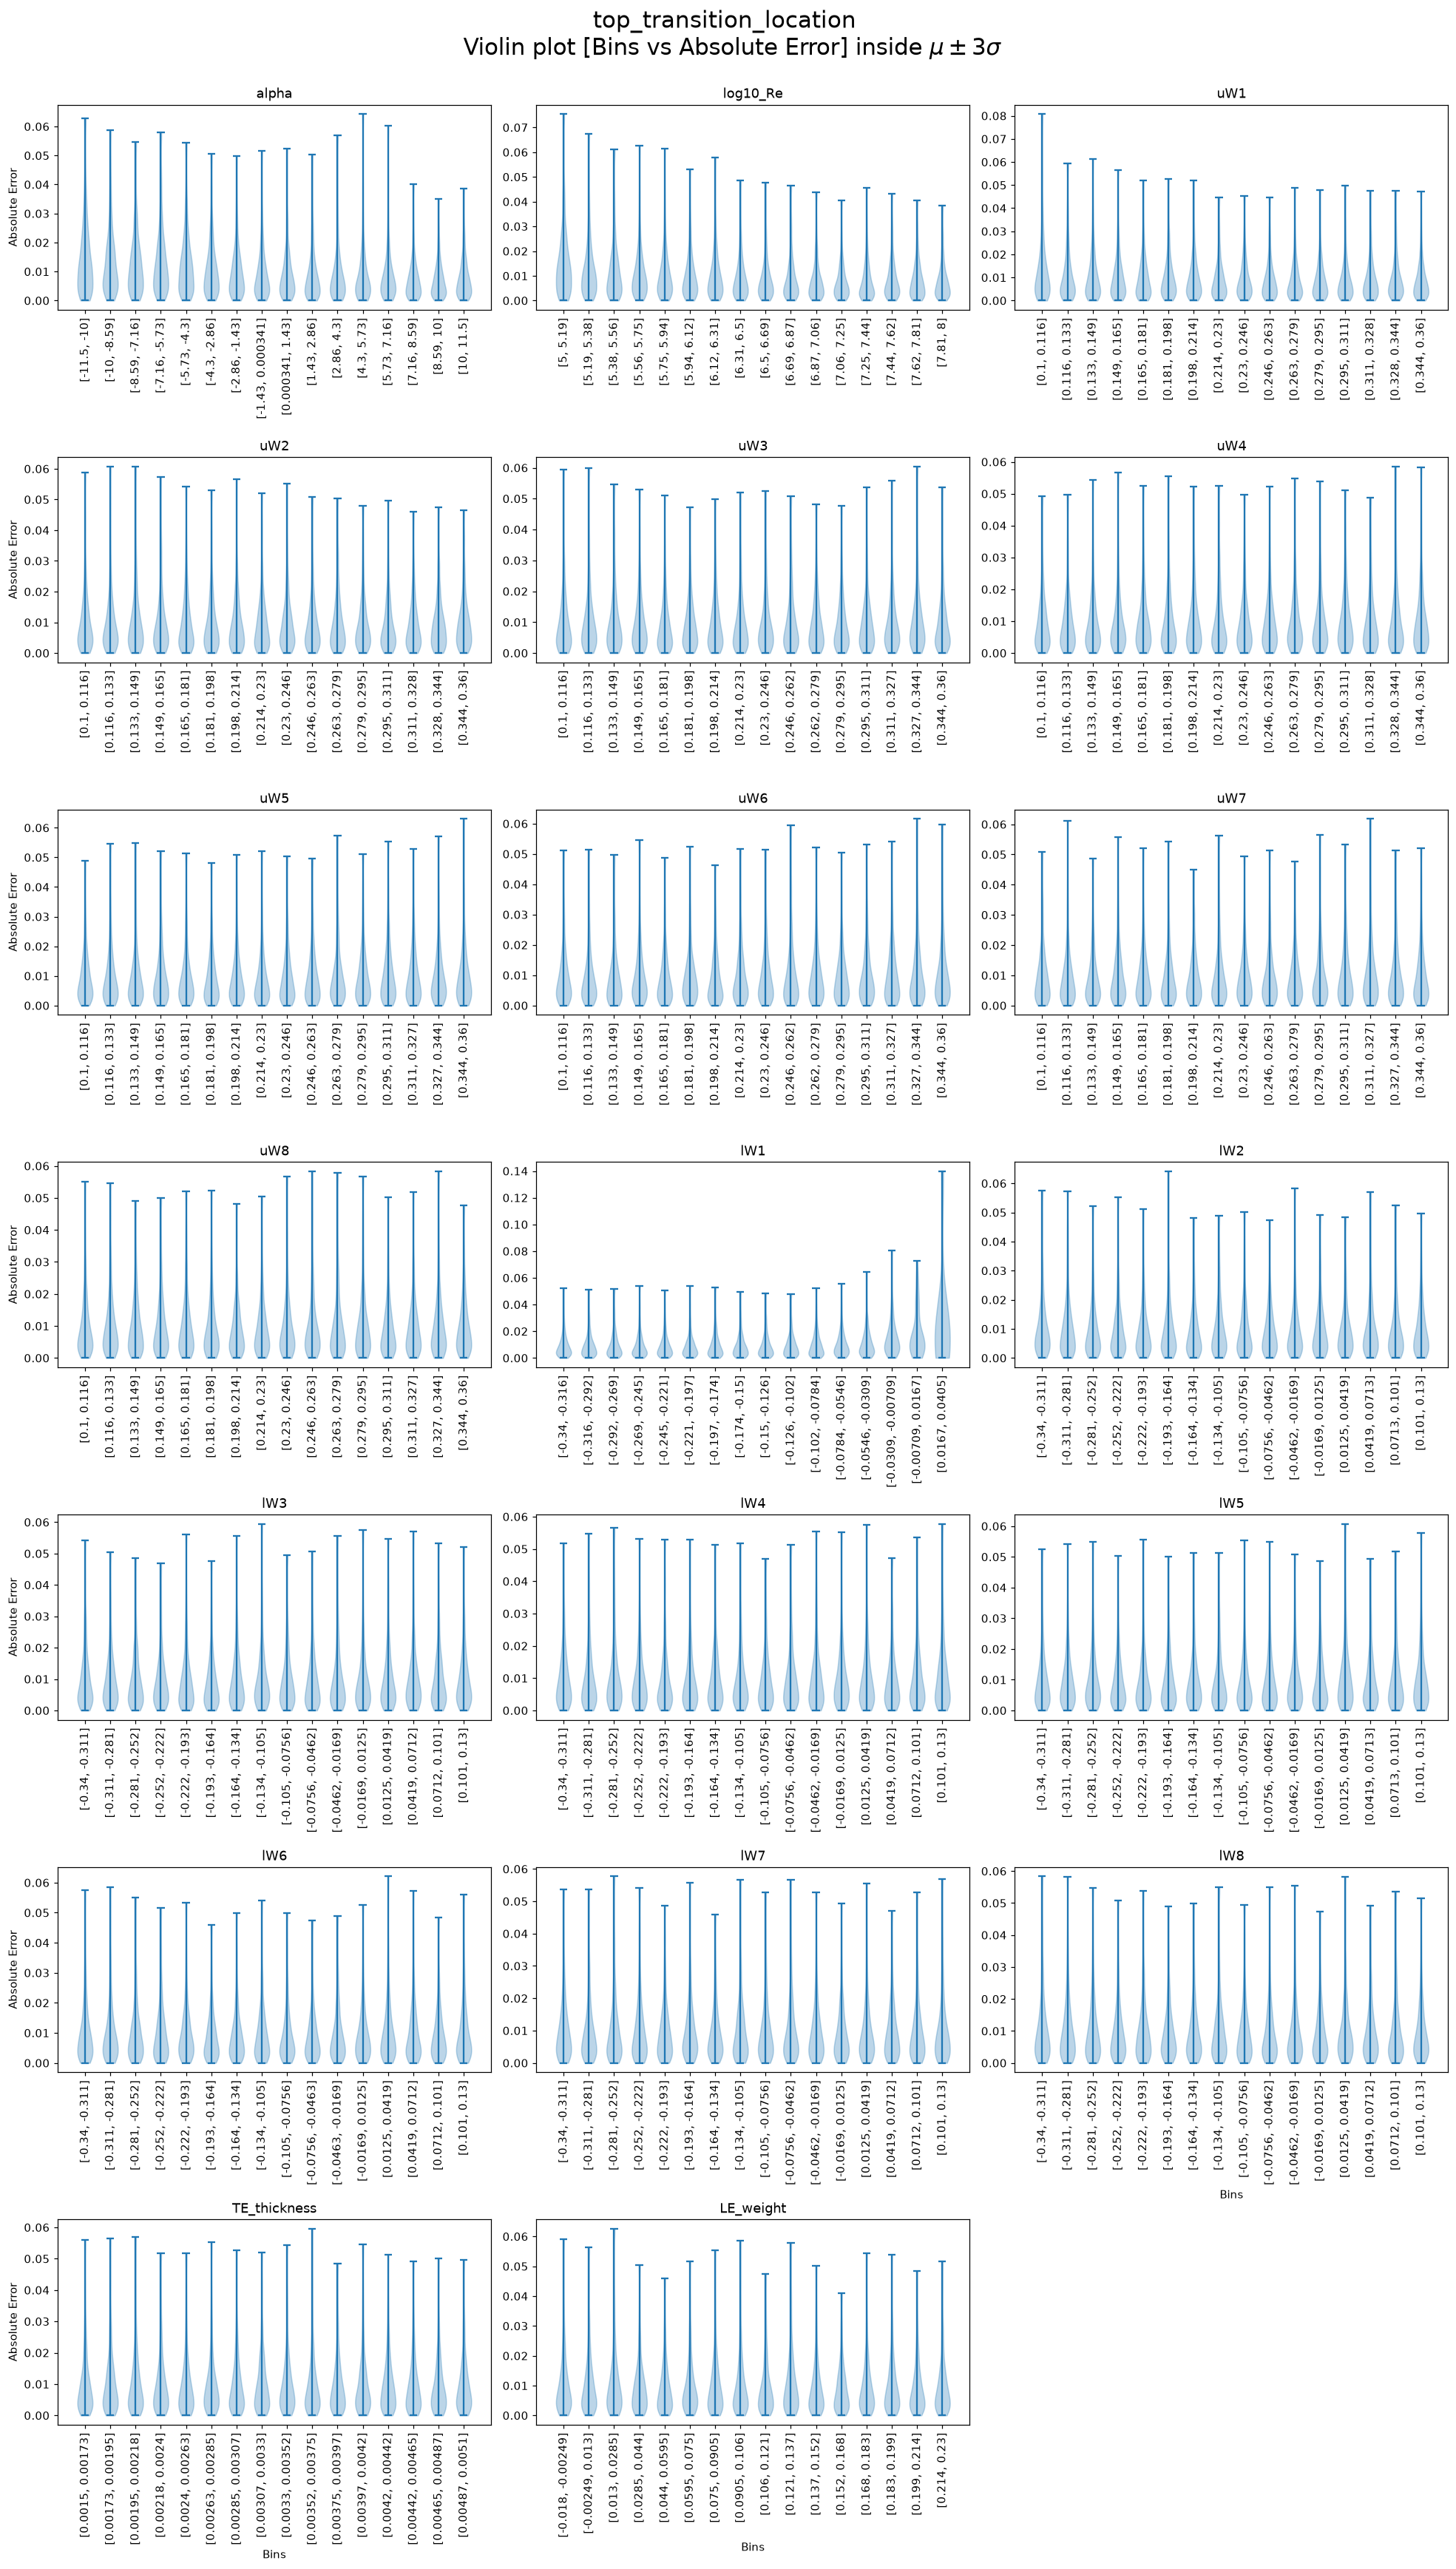
\includegraphics[width=1.0\linewidth,height=0.80\textheight,keepaspectratio]{analysis_plots/pex_violin_abs_top_transition_location.png}\end{center}
\end{minipage}\par\medskip
\par\begin{minipage}{\linewidth}
\subsection*{\normalsize Absolute Error --- bottom\_transition\_location}
\begin{center}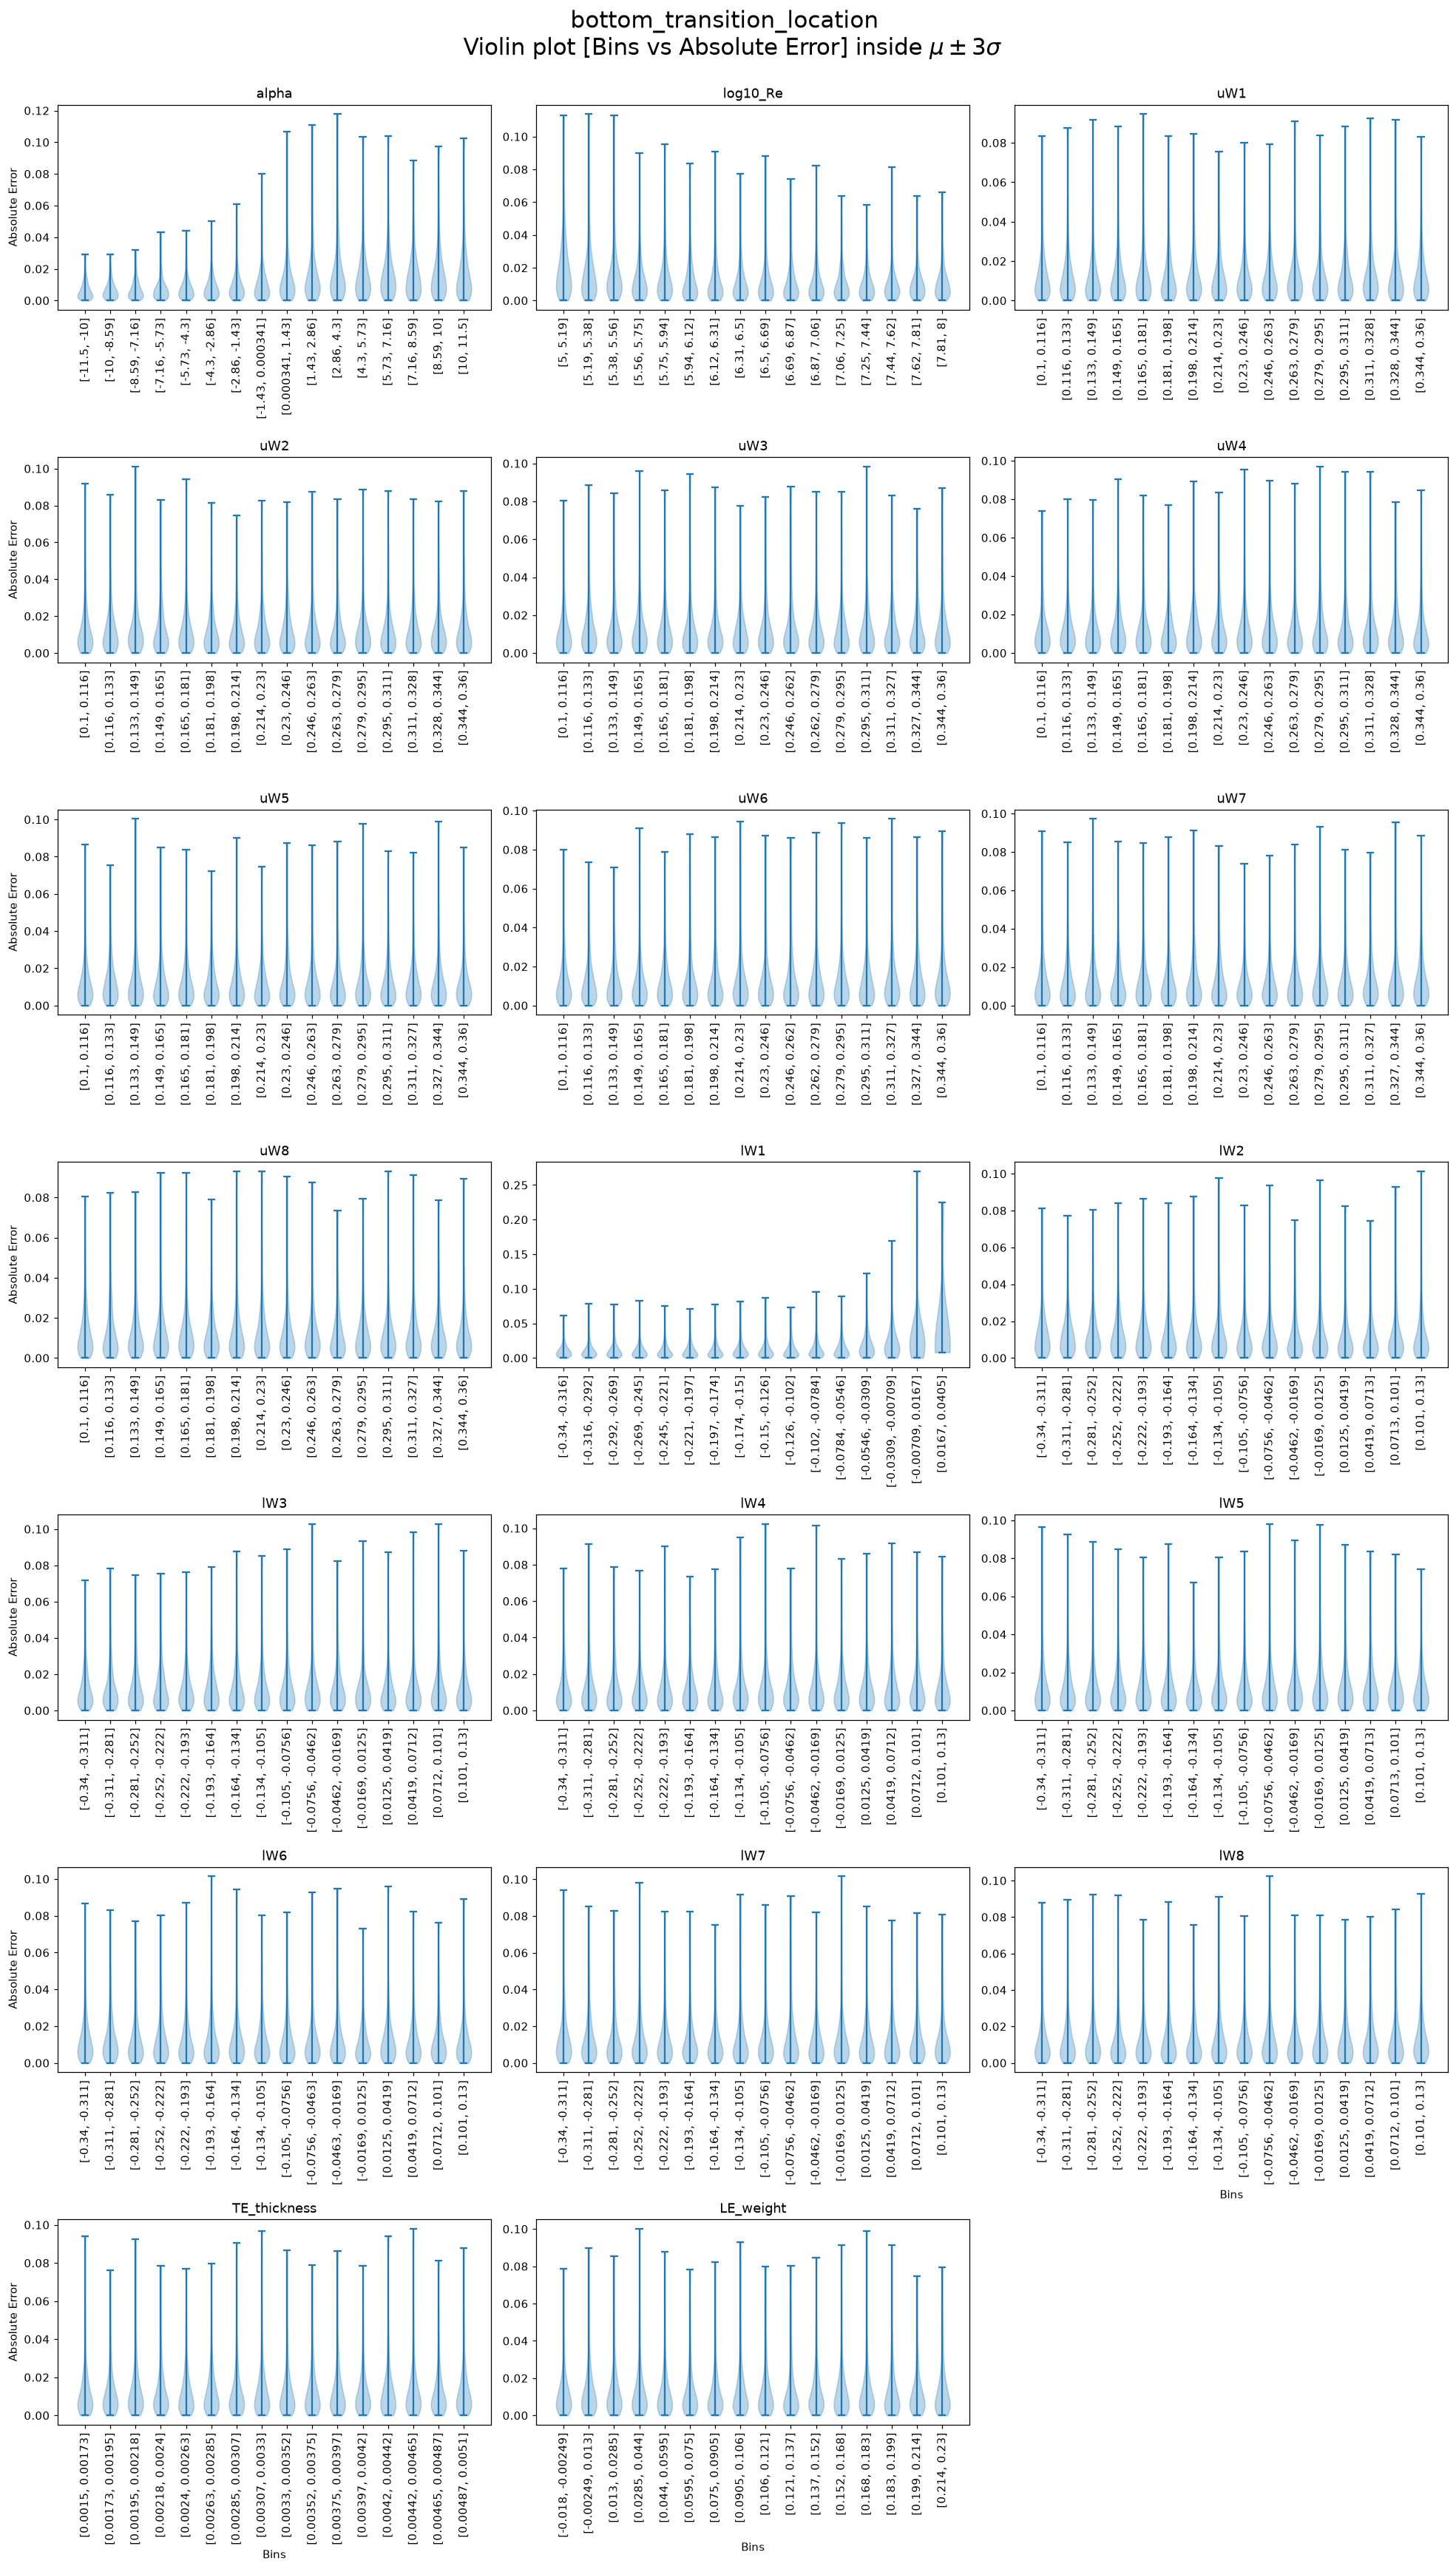
\includegraphics[width=1.0\linewidth,height=0.80\textheight,keepaspectratio]{analysis_plots/pex_violin_abs_bottom_transition_location.png}\end{center}
\end{minipage}\par\medskip
\clearpage
\section{P(E|Y) --- Error Conditional on Outputs}
\label{sec:d5}

We study whether the error depends on the output magnitude. A significant trend (Pearson or Spearman $p<0.05$) means the model is more accurate in some output ranges than others --- a form of heteroscedasticity.

\par\begin{minipage}{\linewidth}
\exhead{Residue vs True Output --- Scatter}
Pearson r and p-value shown in title. Red title = significant linear trend.
\begin{center}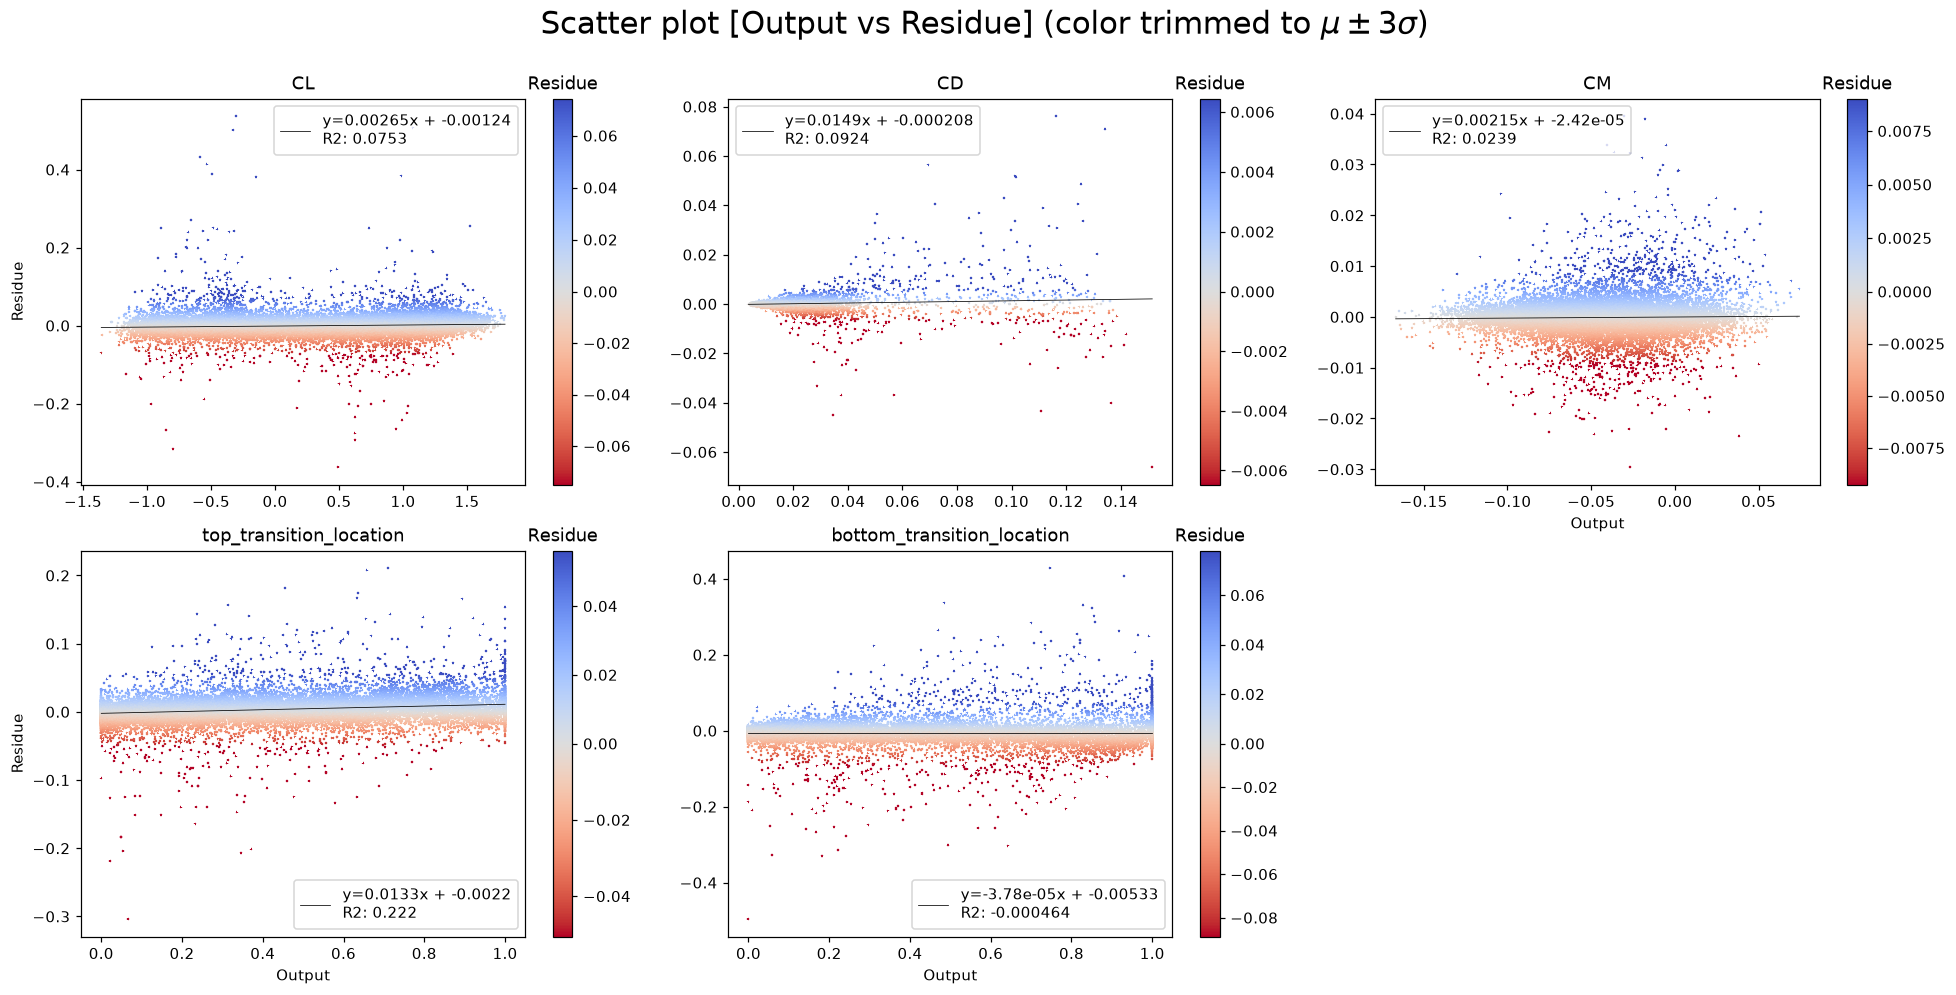
\includegraphics[width=1.0\linewidth,height=0.80\textheight,keepaspectratio]{analysis_plots/pey_residue_scatter.png}\end{center}
\end{minipage}\par\medskip
\par\begin{minipage}{\linewidth}
\exhead{Residue Violin vs True Output Bins}
Bins determined by Sturges rule. Median line dashed at 0.
\begin{center}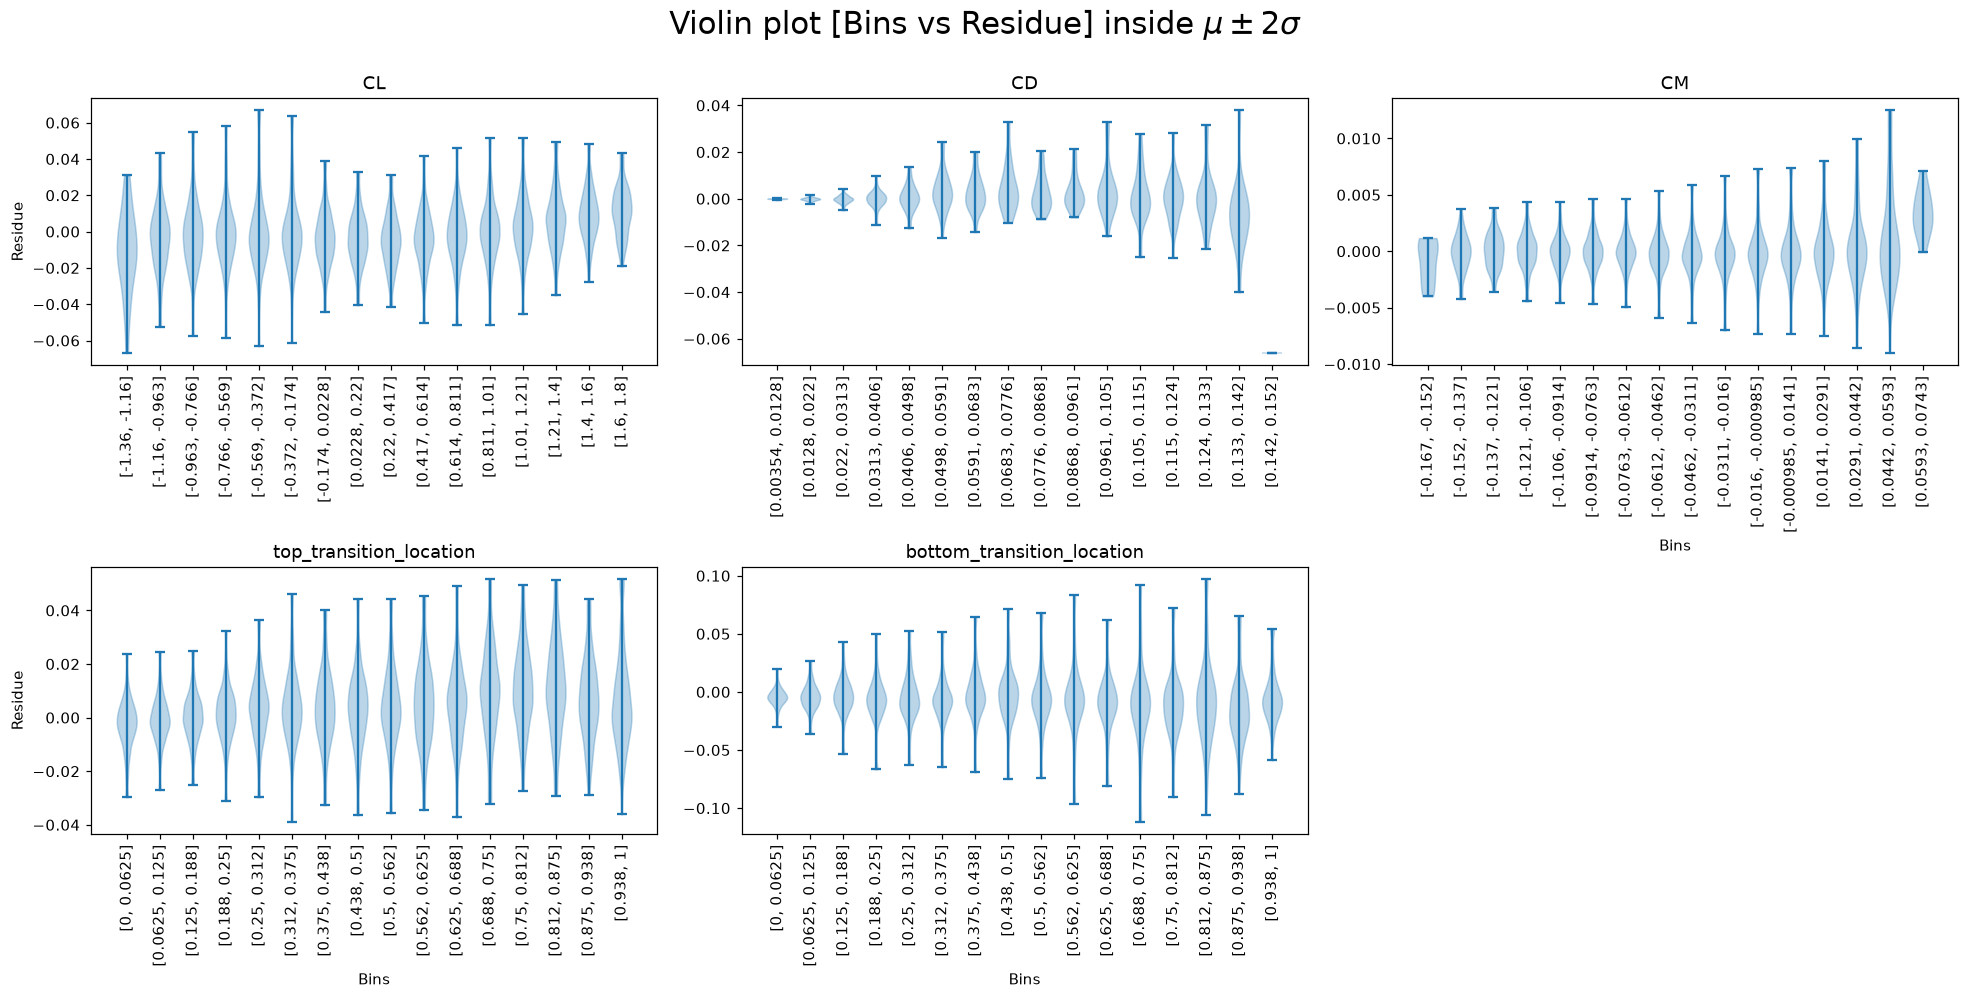
\includegraphics[width=1.0\linewidth,height=0.80\textheight,keepaspectratio]{analysis_plots/pey_residue_violin.png}\end{center}
\end{minipage}\par\medskip
\par\begin{minipage}{\linewidth}
\exhead{Absolute Error vs True Output --- Scatter}
Spearman r shown. Red title = significant monotonic trend.
\begin{center}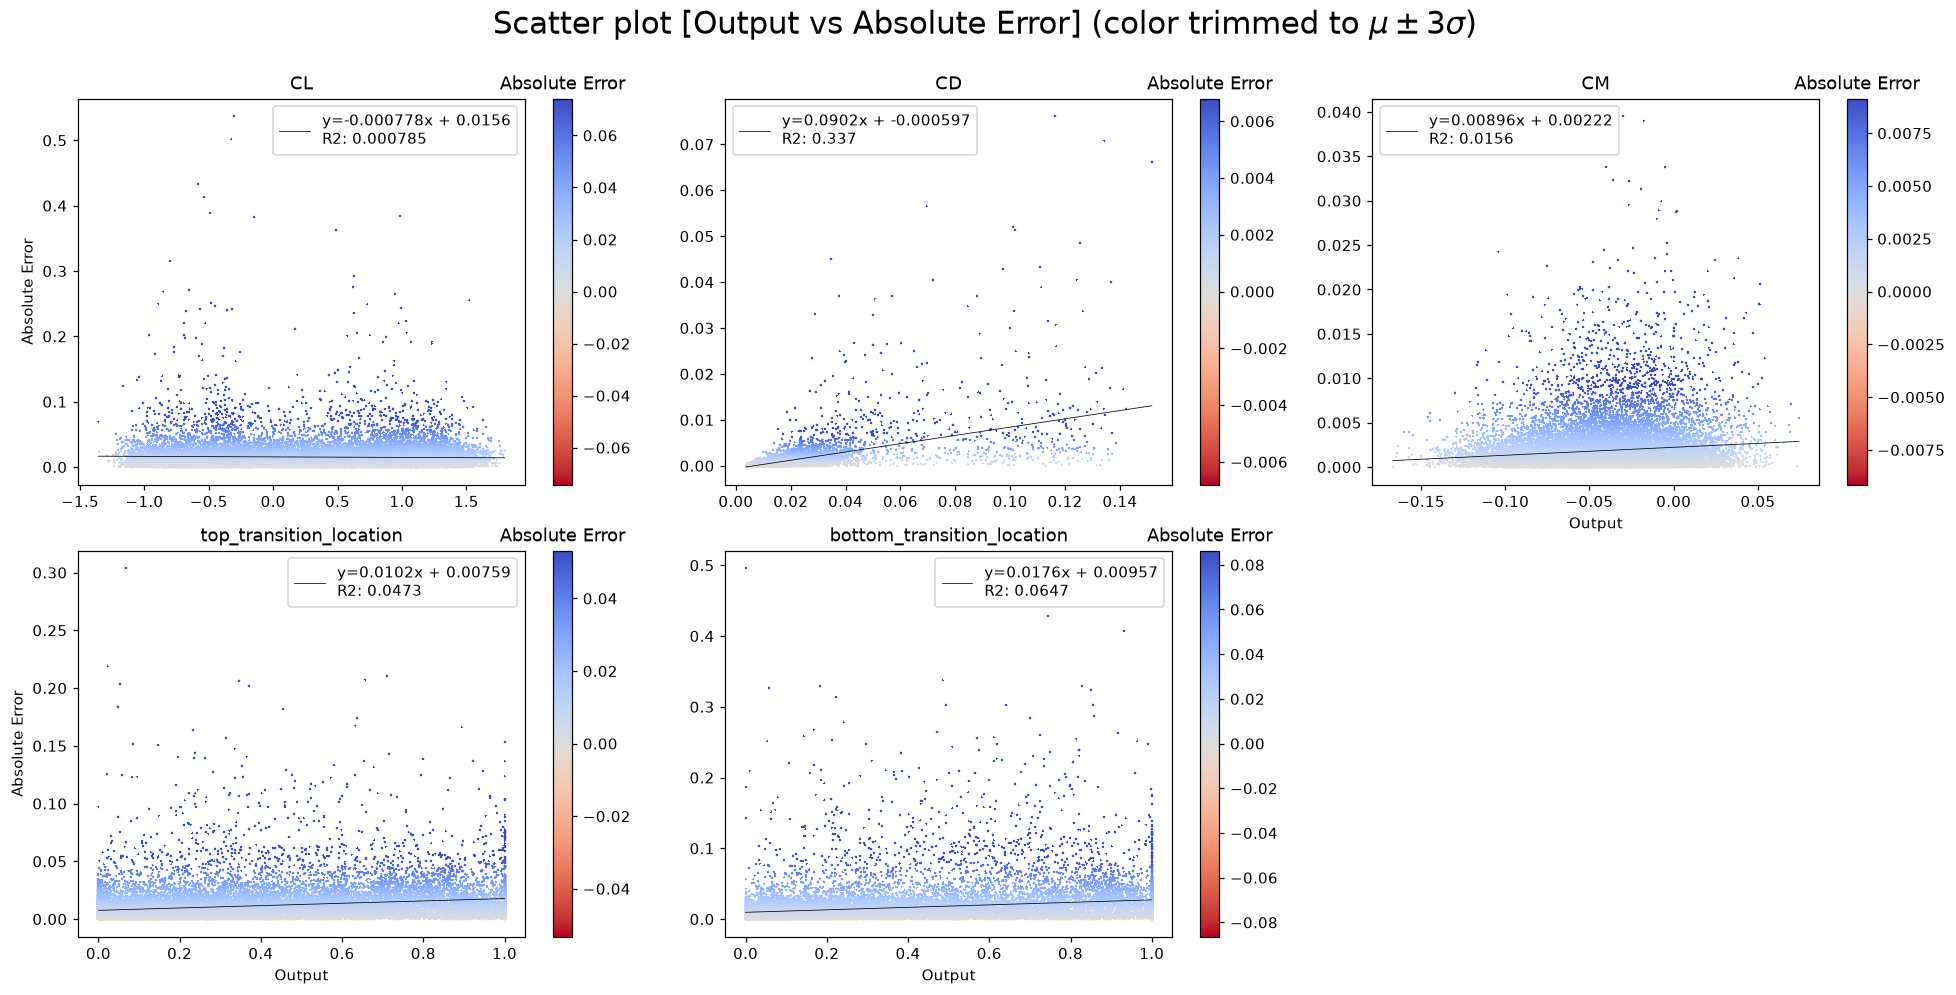
\includegraphics[width=1.0\linewidth,height=0.80\textheight,keepaspectratio]{analysis_plots/pey_abserr_scatter.png}\end{center}
\end{minipage}\par\medskip
\par\begin{minipage}{\linewidth}
\exhead{Absolute Error Violin vs True Output Bins}
\begin{center}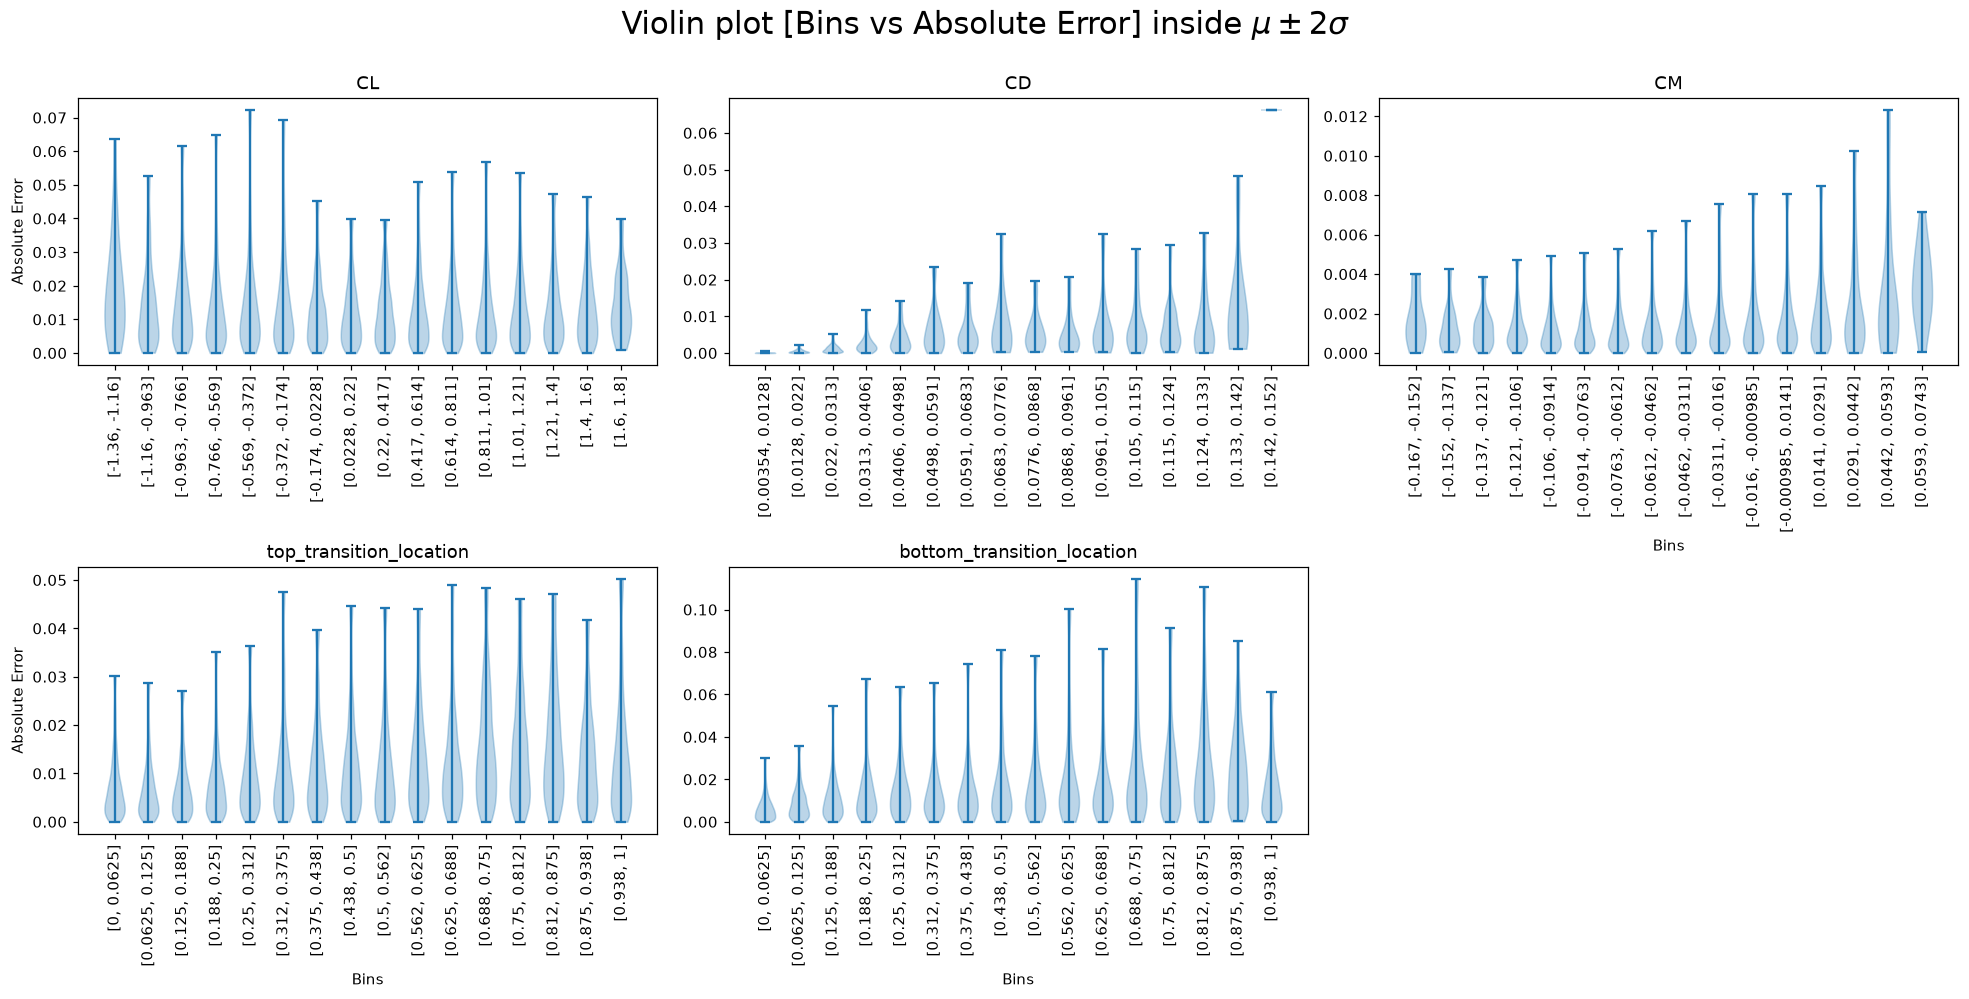
\includegraphics[width=1.0\linewidth,height=0.80\textheight,keepaspectratio]{analysis_plots/pey_abserr_violin.png}\end{center}
\end{minipage}\par\medskip
\clearpage
\section{Uncertainty Analysis}
\label{sec:d6}

A global binned uncertainty model (95th percentile, right-tailed) is trained on the validation split of the absolute error and evaluated on the held-out test split, as in the extended validation notebook. Coverage is the proportion of test points whose error falls inside the predicted bound; it should be close to 95\%.

\par\begin{minipage}{\linewidth}
\exhead{Coverage Plot}
\begin{center}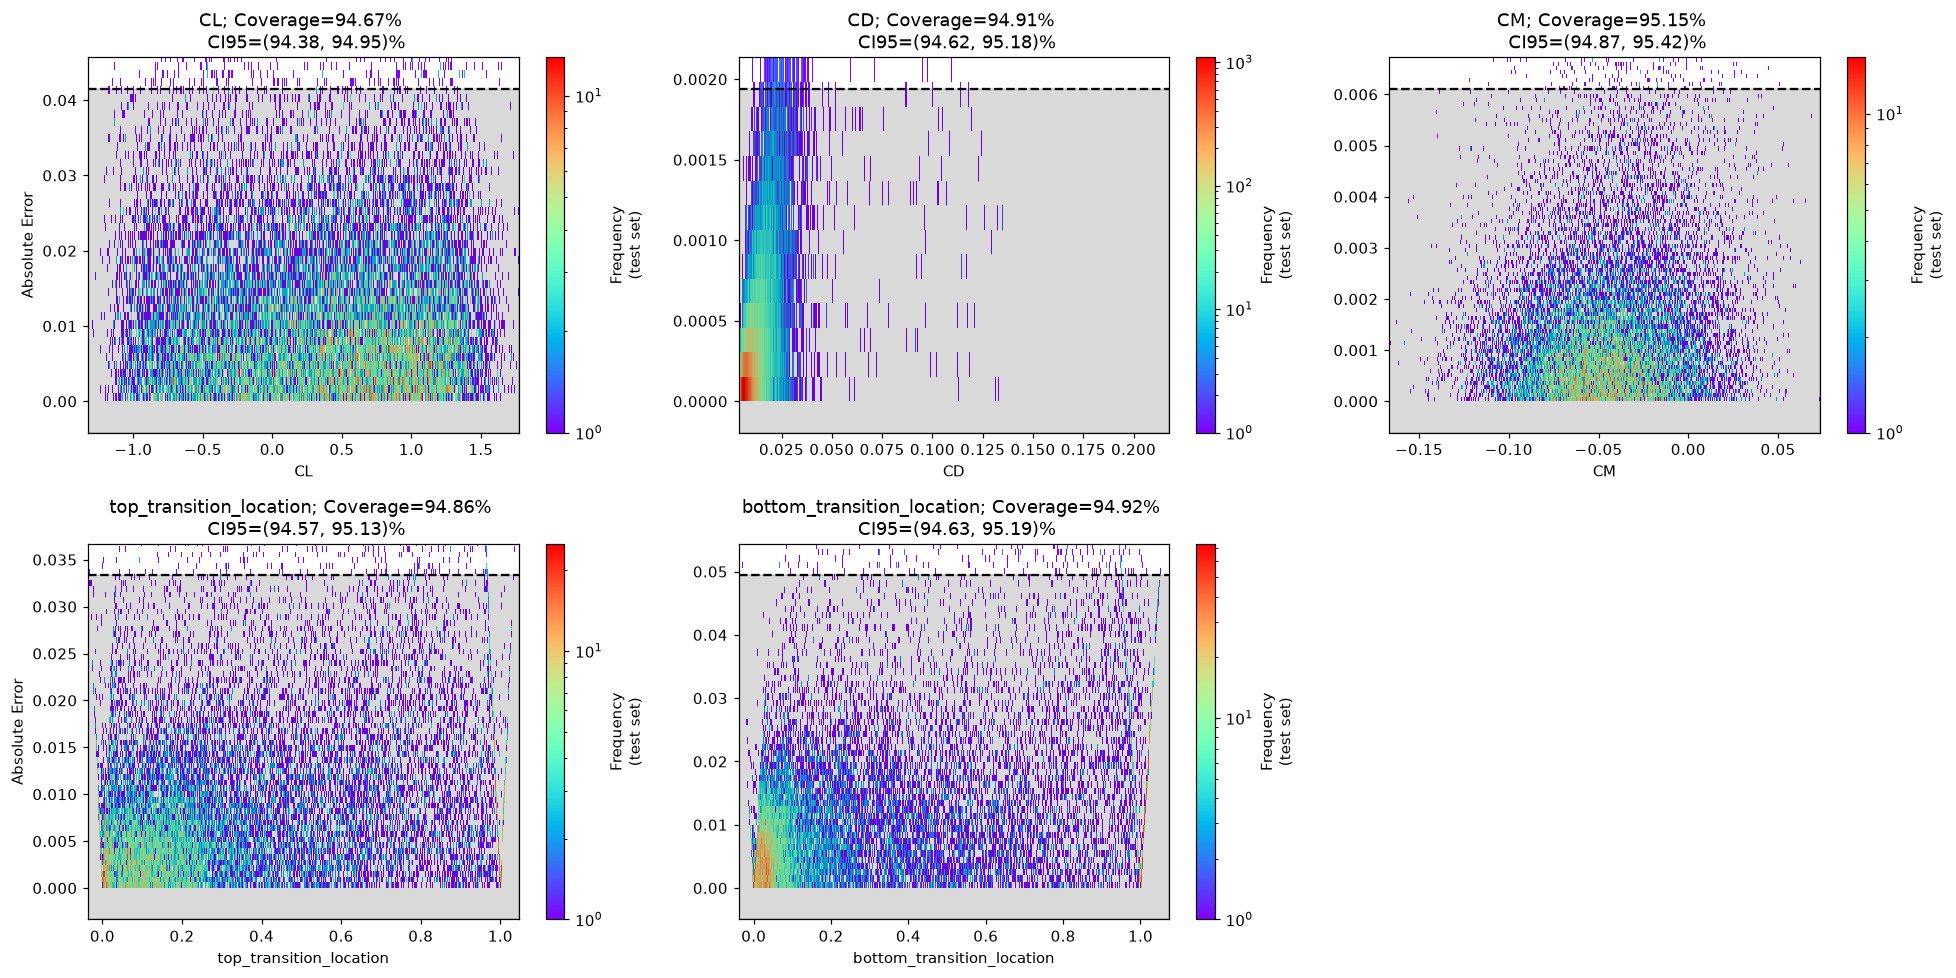
\includegraphics[width=1.0\linewidth,height=0.80\textheight,keepaspectratio]{analysis_plots/uncertainty_coverage.png}\end{center}
\end{minipage}\par\medskip
\exhead{Coverage Table}
\begin{center}
\footnotesize
\renewcommand{\arraystretch}{1.15}
\begin{tabular}{|l|r|r|r|r|r|r|}
\hline
\textbf{} & \textbf{CL} & \textbf{CD} & \textbf{CM} & \textbf{top\_transition\_location} & \textbf{bottom\_transition\_location} & \textbf{TOTAL COV} \\ \hline
\textbf{Coverage} & 94.67 & 94.91 & 95.15 & 94.86 & 94.92 & \textemdash \\ \hline
\textbf{CI} & [94.38, 94.95] & [94.62, 95.18] & [94.87, 95.42] & [94.57, 95.13] & [94.63, 95.19] & \textemdash \\ \hline
\end{tabular}
\par\vspace{2pt}
{\scriptsize Empirical coverage of the 95th-percentile uncertainty bound on the test split.}
\end{center}

\end{document}
